\section{A queueing model for the ED-EMS interface}\label{sec:queueing_model}
In this section, a more in-depth explanation of the queueing model shown in 
figure \ref{fig:diagram_of_queueing_system} will be given.
This is a queueing model that consists of two waiting zones; the parking space
and the hospital waiting space.

\begin{figure}[ht]
    \centering
    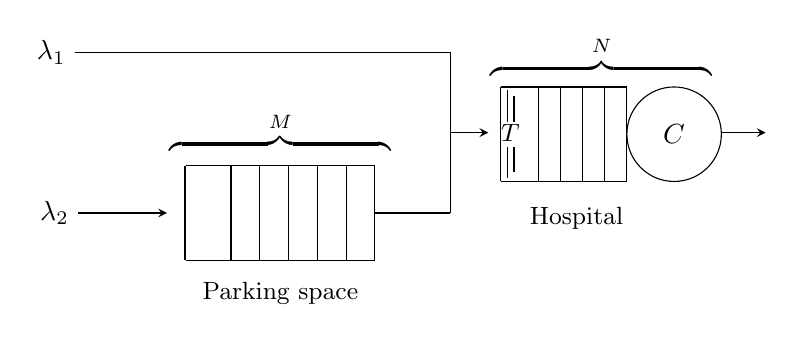
\begin{tikzpicture}[>=stealth, scale=0.8],
        % the rectangle of Queue 1
        \draw (0,0) -- ++(3cm,0) -- ++(0,-1.5cm) -- ++(-3cm,0);
        % The label above Queue 1 -> M
        \node[anchor=north] at (1.5cm, 1cm) {\( 
            \overbrace{\qquad \qquad \qquad \qquad}^{M} 
        \)};
        % The label below Queue 1 -> Parking space
        \node[anchor=north] at (1.5cm, -1.7cm) {\small{Parking space}};

        % the vertical lines in Queue 1
        \foreach \i in {1,...,5, 6.6}
        \draw (3cm-\i*13pt,0) -- +(0,-1.5cm);
        
        % % the circle in Queue 1
        % \draw (2.75,-0.75cm) circle [radius=0.75cm] node {\(0\)};

        % the rectangle in Queue 2
        \draw (5,1.25) -- ++(2cm,0) -- ++(0,-1.5cm) -- ++(-2cm,0);
        % the vertical lines in Queue 2
        \foreach \i in {1,...,4, 5.7}
        \draw (7cm-\i*10pt,1.25) -- +(0,-1.5cm);
        % The two vertical lines at the start of Queue 2 
        \draw (7cm-54pt,1.2) -- +(0,-0.5cm);
        \draw (7cm-54pt,0.3) -- +(0,-0.5cm);        
        \draw (7cm-51pt,1.1) -- +(0,-0.4cm);
        \draw (7cm-51pt,0.3) -- +(0,-0.4cm);

        % The label between the lines for T
        \node[anchor=north] at (5.15, 0.81 cm) {\small{\( T \)}};

        % The label above Queue 2 -> N
        \node[anchor=north] at (6.6cm, 2.2cm) {\( 
            \overbrace{\qquad \qquad \qquad \qquad}^{N} 
        \)};
        % The label below Queue 2 -> Hospital
        \node[anchor=north] at (6.2cm, -0.5cm) {\small{Hospital}};

        % the circle in Queue 2
        \draw (7.75,0.5) circle [radius=0.75cm] node {\(C\)};

        % Arrow line from Queue 2 outside
        \draw[->] (8.5,0.525) -- +(20pt,0);
        
        % Line from lambda_2 to Queue 1
        \draw[<-] (-0.3,-0.75) -- +(-40pt,0) node[left] {\( \lambda_2 \)};
        % First line (horizontal) after Queue 1
        \draw[-] (3,-0.75) -- +(34pt,0);
        % Second line (vertical) after Queue 1
        \draw (4.2, 0.525) -- (4.2, -0.75);
        
        % First line (horizontal) from lambda_1
        \draw (4.2, 1.8) -- +(-169.5pt,0) node[left] {\( \lambda_1 \)};
        % Second line (vertical) from lambda_1
        \draw (4.2, 1.8) -- (4.2, 0.525);
        % Arrow line to Queue 2
        \draw[->] (4.2, 0.525) -- (4.8, 0.525);  
    \end{tikzpicture}
    \caption{A diagrammatic representation of the queueing model. 
    The threshold \(T\) only applies to type 2 individuals.
    If the number of individuals in the hospital is \(T\), only 
    individuals of type 1 
    are accepted (at a rate \(\lambda_1\)) and individuals of type 2
    (arriving at a rate \(\lambda_2\)) are blocked in the parking space.}
    \label{fig:diagram_of_queueing_system}
\end{figure}

The model consists of two types of individuals; type 1 and type 2.
Type 2 individuals are patients arriving in ambulances who can be blocked 
(usually patients that are deemed not to be critical) 
and type 1 individuals are individuals arriving from other sources 
(e.g walk-in patients, urgent patients from either walk-ins or ambulances).
Type 1 individuals arrive instantly at the hospital's waiting space and wait to
receive their service. 
Type 2 individuals arrive at the parking space and wait there until they are 
allowed to move to the hospital.
They are allowed to proceed only when the number of 
patients in the hospital is less than the
pre-determined threshold \(T\).
When the number of individuals is equal to or exceeds this threshold, all 
type 2 patients that arrive will stay 
\textit{blocked} in the parking space until the number of patients in 
the hospital falls below \(T\). 
This is shown diagrammatically in Figure \ref{fig:diagram_of_queueing_system}.
The parameters of the described queueing model are:

\begin{itemize}
    \item \(\lambda_i\): The arrival rate of individuals of type 
    \(i\in\{1, 2\}\)
    \item \(\mu\): The service rate for individuals receiving service
    \item \(C\): The number of servers (either healthcare professionals
    or available beds in the ED)
    \item \(T\): The threshold at which type 2 individuals are blocked
\end{itemize}

Under the assumption that all rates (arrival and service) are Markovian the
queueing system corresponds to a Markov chain~\cite{kemeny1976markov}.
The states of the Markov chain are denoted by \((u,v)\) where:

\begin{itemize}
    \item \(u\) is the number of individuals blocked in the parking space
    \item \(v\) is the number of individuals waiting or being served in the
    hospital
\end{itemize}

We denote the state space of the Markov chain as  \(S=S(T)\) which can be 
written as the disjoint union (\ref{eq:definition_of_S_as_disjoint_union}).

\begin{align}
    S(T) =& S_1(T) \cup S_2(T) \text{ where:} \nonumber \\
    S_1(T) =& \left\{(0, v)\in\mathbb{N}_0^2 \; | \; v < T \right\} 
    \label{eq:definition_of_S_as_disjoint_union} \\
    S_2(T) =& \{(u, v)\in\mathbb{N}_0^2 \; | \; v \geq T \} \nonumber
\end{align}

The generator matrix \(Q\) of the Markov chain consists of the 
rates between the numerous states of the model. 
Every entry \( Q_{ij} = Q_{(u_i, v_i),(u_j, v_j)} \) represents the rate from 
state \( i = (u_i, v_i) \) to state \( j = (u_j , v_j) \) for all 
\( (u_i, v_i), (u_j, v_j) \in S \).
The entries of \(Q\) can be calculated using the state-mapping function 
described in (\ref{eq:markov_transition_rate}): 

\begin{equation} \label{eq:markov_transition_rate}
    Q_{ij} = 
    \begin{cases}
        \Lambda, & \textbf{if } (u_i, v_i) - (u_j, v_j) = (0,-1) \textbf{ and } 
        v_i < \text{t} \\
        \lambda_1, & \textbf{if } (u_i, v_i) - (u_j, v_j) = (0,-1) 
        \textbf{ and } v_i \geq \text{t} \\
        \lambda_2, & \textbf{if } (u_i, v_i) - (u_j, v_j) = (-1,0) \\
        v_i \mu, & \textbf{if } (u_i, v_i) - (u_j, v_j) = (0,1) \textbf{ and } 
        v_i \leq C \textbf{ or} \\ & \hspace{0.37cm}(u_i, v_i) - (u_j, v_j) = 
        (1,0) \textbf{ and } v_i = T \leq C \\
        C \mu, & \textbf{if } (u_i, v_i) - (u_j, v_j) = (0,1) \textbf{ and } 
        v_i > C 
        \textbf{ or} \\ & \hspace{0.37cm}(u_i, v_i) - (u_j, v_j) = (1,0) 
        \textbf{ and } v_i = T > C\\
        -\sum_{j=1}^{|Q|}{Q_{ij}} & \textbf{if } i = j \\
        0, & \textbf{otherwise}
    \end{cases}
\end{equation}

Note that \(\Lambda\) here denotes the overall arrival rate in the model by both 
types of individuals (i.e. \(\Lambda = \lambda_1 + \lambda_2\)). 
A visualisation of how the transition rates relate to the states of the model 
can be seen in the general Markov chain model shown in Figure 
\ref{fig:general_markov_model}.

\documentclass{article}

\usepackage{amsmath}
\usepackage{amsfonts} 
\usepackage{geometry}
\usepackage{multicol}
\usepackage{float}
% \usepackage{mathtools}
% \usepackage{graphicx}
% \usepackage{soul}
% \usepackage{indentfirst}
\usepackage{tikz}
\usetikzlibrary{calc, automata, chains, arrows.meta, math}
\setcounter{MaxMatrixCols}{20}


\title{A game theoretic model of the behavioural gaming that takes place at the EMS - ED interface}

\author{
    Michalis Panayides, 
    Paul Harper, 
    Vince Knight
}

\begin{document}

\maketitle

\documentclass{article}

\usepackage{amsmath}
\usepackage{amsfonts} 
\usepackage{geometry}
\usepackage{multicol}
\usepackage{float}
% \usepackage{mathtools}
% \usepackage{graphicx}
% \usepackage{soul}
% \usepackage{indentfirst}
\usepackage{tikz}
\usetikzlibrary{calc, automata, chains, arrows.meta, math}
\setcounter{MaxMatrixCols}{20}


\title{A game theoretic model of the behavioural gaming that takes place at the EMS - ED interface}

\author{
    Michalis Panayides, 
    Paul Harper, 
    Vince Knight
}

\begin{document}

\maketitle

\documentclass{article}

\usepackage{amsmath}
\usepackage{amsfonts} 
\usepackage{geometry}
\usepackage{multicol}
\usepackage{float}
% \usepackage{mathtools}
% \usepackage{graphicx}
% \usepackage{soul}
% \usepackage{indentfirst}
\usepackage{tikz}
\usetikzlibrary{calc, automata, chains, arrows.meta, math}
\setcounter{MaxMatrixCols}{20}


\title{A game theoretic model of the behavioural gaming that takes place at the EMS - ED interface}

\author{
    Michalis Panayides, 
    Paul Harper, 
    Vince Knight
}

\begin{document}

\maketitle

\input{Abstract/main.tex}


\newpage
\tableofcontents

\newpage
\input{Introduction/main.tex}

\newpage
\input{Game_theory_component/main.tex}

\newpage
\input{MarkovChain/markov_chain_model/main.tex}
\input{MarkovChain/expressions_from_pi/main.tex}
\input{MarkovChain/markov_example/main.tex}

\newpage
\input{BehaviouralMethodology/main.tex}

\newpage
\input{Application_EMS_ED/main.tex}

\newpage
\input{Conclusion/main.tex}


\end{document}


\newpage
\tableofcontents

\newpage
\documentclass{article}

\usepackage{amsmath}
\usepackage{amsfonts} 
\usepackage{geometry}
\usepackage{multicol}
\usepackage{float}
% \usepackage{mathtools}
% \usepackage{graphicx}
% \usepackage{soul}
% \usepackage{indentfirst}
\usepackage{tikz}
\usetikzlibrary{calc, automata, chains, arrows.meta, math}
\setcounter{MaxMatrixCols}{20}


\title{A game theoretic model of the behavioural gaming that takes place at the EMS - ED interface}

\author{
    Michalis Panayides, 
    Paul Harper, 
    Vince Knight
}

\begin{document}

\maketitle

\input{Abstract/main.tex}


\newpage
\tableofcontents

\newpage
\input{Introduction/main.tex}

\newpage
\input{Game_theory_component/main.tex}

\newpage
\input{MarkovChain/markov_chain_model/main.tex}
\input{MarkovChain/expressions_from_pi/main.tex}
\input{MarkovChain/markov_example/main.tex}

\newpage
\input{BehaviouralMethodology/main.tex}

\newpage
\input{Application_EMS_ED/main.tex}

\newpage
\input{Conclusion/main.tex}


\end{document}

\newpage
\documentclass{article}

\usepackage{amsmath}
\usepackage{amsfonts} 
\usepackage{geometry}
\usepackage{multicol}
\usepackage{float}
% \usepackage{mathtools}
% \usepackage{graphicx}
% \usepackage{soul}
% \usepackage{indentfirst}
\usepackage{tikz}
\usetikzlibrary{calc, automata, chains, arrows.meta, math}
\setcounter{MaxMatrixCols}{20}


\title{A game theoretic model of the behavioural gaming that takes place at the EMS - ED interface}

\author{
    Michalis Panayides, 
    Paul Harper, 
    Vince Knight
}

\begin{document}

\maketitle

\input{Abstract/main.tex}


\newpage
\tableofcontents

\newpage
\input{Introduction/main.tex}

\newpage
\input{Game_theory_component/main.tex}

\newpage
\input{MarkovChain/markov_chain_model/main.tex}
\input{MarkovChain/expressions_from_pi/main.tex}
\input{MarkovChain/markov_example/main.tex}

\newpage
\input{BehaviouralMethodology/main.tex}

\newpage
\input{Application_EMS_ED/main.tex}

\newpage
\input{Conclusion/main.tex}


\end{document}

\newpage
\documentclass{article}

\usepackage{amsmath}
\usepackage{amsfonts} 
\usepackage{geometry}
\usepackage{multicol}
\usepackage{float}
% \usepackage{mathtools}
% \usepackage{graphicx}
% \usepackage{soul}
% \usepackage{indentfirst}
\usepackage{tikz}
\usetikzlibrary{calc, automata, chains, arrows.meta, math}
\setcounter{MaxMatrixCols}{20}


\title{A game theoretic model of the behavioural gaming that takes place at the EMS - ED interface}

\author{
    Michalis Panayides, 
    Paul Harper, 
    Vince Knight
}

\begin{document}

\maketitle

\input{Abstract/main.tex}


\newpage
\tableofcontents

\newpage
\input{Introduction/main.tex}

\newpage
\input{Game_theory_component/main.tex}

\newpage
\input{MarkovChain/markov_chain_model/main.tex}
\input{MarkovChain/expressions_from_pi/main.tex}
\input{MarkovChain/markov_example/main.tex}

\newpage
\input{BehaviouralMethodology/main.tex}

\newpage
\input{Application_EMS_ED/main.tex}

\newpage
\input{Conclusion/main.tex}


\end{document}
\subsection{Performance Measures}
One may easily derive the average number of individuals that are at any given state 
using \( pi \). 
The average number of individuals in state \( i \) can be calculated by multiplying 
the number of individuals that are present in state \( i \) with the probability 
of being at that particular state (i.e \(\pi_i (u_i + v_i)\)). 
Using this logic it is possible to calculate any performance measures that are related 
to the mean number of individuals in the system.


Average number of people in the system: 
\begin{equation}
    L = \sum_{i=1}^{|\pi|} \pi_i (u_i + v_i)
\end{equation} 

Average number of people in the service centre: 
\begin{equation}
    L_H = \sum_{i=1}^{|\pi|} \pi_i v_i
\end{equation}

Average number of people in the buffer centre:
\begin{equation}
    L_A = \sum_{i=1}^{|\pi|} \pi_i u_i
\end{equation}

Consequently getting the performance measures that are related to the duration of 
time is not as straightforward. 
Such performance measures are the mean waiting time in the system and the mean time 
blocked in the system. 
Under the scope of this study three approaches have been considered to calculate these 
performance measures; a direct approach, a recursive algorithm and consequently a
closed-form formula.

The research question that needs to be answered here is: ``When a class 1/2 
individuals enters the system, what is the expected time that they will have to 
wait?''. 
In order to formulate the answer to that question one needs to consider all possible 
scenarios of what state the system can be in when an individual arrives. 
Furthermore, different formulas arises for class 1 individuals 
and a different one for class 2 individuals.

\subsubsection{Mean waiting time} 
Upon closer inspection of the recursive formula a more compact formula can arise. 
The equivalent closed-form formula eliminates the need for recursion and thus makes 
the computation of waiting times much more efficient. 
Just like in the recursive part there are two formulas; one for \textit{class 1} 
and one for class 2 individuals. 
The formulas are given by:

\begin{equation} \label{eq:closed_form_waiting_others}
    W^{(1)} = \frac{\sum_{\substack{(u,v) \, \in S_A^{(1)} \\ v \geq C}} 
    \frac{1}{C \mu} \times (v-C+1) \times \pi(u,v)}{\sum_{(u,v) \, 
    \in S_A^{(1)}} \pi(u,v)}
\end{equation}
    
\begin{equation}\label{eq:closed_form_waiting_ambulance}
    W^{(2)} = \frac{\sum_{\substack{(u,v) \, \in S_A^{(2)} \\ min(v,T) \geq C}} 
    \frac{1}{C \mu} \times (\min(v+1,T)-C) \times \pi(u,v)}{\sum_{(u,v) \, 
    \in S_A^{(2)}} \pi(u,v)}
\end{equation}

Note here that the summation, in both equations \ref{eq:closed_form_waiting_others} 
and \ref{eq:closed_form_waiting_ambulance}, goes through all states in the set of 
accepting 
states of either class 1 or class 2 individuals respectively, where a wait 
incurs. 
In equation \ref{eq:closed_form_waiting_others} that includes all states \((u,v)\) 
in the set of accepting states of class 1 individuals such that \( v \geq C\); i.e. 
whenever an arrival occurs and the system is at a state where the number of individuals 
in the system is more than or equal to $C$. 
Consequently, for the states that are included in the summation the expression 
\( v-C+1 \) indicates the amount of people in service one would have to wait for 
upon arrival at the hospital.

Additionally, the minimisation function in equation 
\ref{eq:closed_form_waiting_ambulance} 
ensures that when a class 2 individual arrives at any state 
that is greater than the predetermined threshold, the wait that the individual will 
have to endure remains the same. 
In essence, the expression \(\min(v+1,T) - C\) returns the number of people in line 
in front of a particular individual upon arrival.


\subsubsection{Overall Waiting Time}

Consequently, the overall waiting time should can be estimated by a linear combination 
of the waiting times of class 1 and class 2 individuals. 
The overall waiting time can be then given by the following equation where \(c_1\) 
and \(c_2\) are the coefficients of each individual's type waiting time:

\begin{equation}\label{overall_waiting_time_coeff}
    W = c_1 W^{(1)} + c_2 W^{(2)}
\end{equation}

The two coefficients represent the proportion of individuals of each type that 
traversed through the model. 
Theoretically, getting these percentages should be as simple as looking at the arrival 
rates of each type but in practise if the service centre or the buffer centre 
is full, some individuals may be lost to the system. 
Thus, one should account for the probability that an individual is lost to the system. 
This probability can be easily calculated by using the two sets of accepting states 
\(S_A^{(2)}\) and \(S_A^{(1)}\) defined earlier in equations.
Let us define here the probability, for either class type, that an individual 
is not lost in the system by:

\begin{equation*}
    P(L'_1) = \sum_{(u,v) \, \in S_A^{(1)}} \pi(u,v) \hspace{2cm}
    P(L'_2) = \sum_{(u,v) \, \in S_A^{(2)}} \pi(u,v)
\end{equation*}

Having defined these probabilities one may combine them with the arrival rates of 
each class type in such a way to get the expected proportions of class 1 and 
class 2 individuals in the model. 
Thus, by using these values as the coefficient of equation 
\ref{overall_waiting_time_coeff} 
the resultant equation can be used to get the overall waiting time. 
Note here that the equation below gets the overall waiting time for both the recursive 
and the closed-form formula.

\begin{equation}\label{overall_waiting_time}
    W = \frac{\lambda_1 P(L'_1)}{\lambda_2 P(L'_2) + \lambda_1 P(L'_1)} W^{(1)} + 
    \frac{\lambda_2 P(L'_2)}{\lambda_2 P(L'_2) + \lambda_1 P(L'_1)} W^{(2)}
\end{equation}



\subsubsection{Mean blocking time}
Unlike the waiting time, the blocking time is only calculated for class 2 individuals.  
That is because class 1 individuals cannot be blocked. 
Thus, one only needs to consider the pathway of class 2 individuals to get the 
mean blocking time of the system. 
Blocking occurs at states \((u,v)\) where \(u > 0 \). 
Thus, the set of blocking states can be defined as:

\begin{equation*}
    S_b = \{(u,v) \in S \; | \; u > 0\}
\end{equation*}
 
In order to not consider individuals that will be lost to the system, the set of 
accepting states needs to be taken into account. The set of accepting states is given by:

\begin{equation*}
    S_A^{(2)}=
    \begin{cases}
        \{(u, v) \in S \; | \; u < M \} & \textbf{if } T \leq N\\
        \{(u, v) \in S \; | \; v < N \} & \textbf{otherwise}
    \end{cases}
\end{equation*}

For the waiting time formula,
the mean sojourn time for each state was considered,
ignoring any arrivals. Here, the same approach is used but ignoring only class 2
arrivals. That is because for the waiting time formula, once an individual enters 
the service centre (i.e. starts waiting) any individual arriving after them will 
not affect their
pathway. That is not the case for blocking time. When a class 2 individual is 
blocked, 
any class 1 individual that arrives will cause the blocked individual to remain 
blocked for more time. Therefore, class 1 arrivals are considered here:

\begin{equation}\label{eq:time_in_state_blocking_time}
    c(u,v) = 
    \begin{cases}
        \frac{1}{\min(v,C) \mu}, & \text{if } v = C\\
        \frac{1}{\min(v,C) \mu + \lambda_1}, & \text{otherwise}
    \end{cases}
\end{equation}
 
In equation \ref{eq:time_in_state_blocking_time}, both service completions and 
class 1 arrivals are considered. 
Thus, from a blocked individual's perspective whenever the system moves from one 
state \((u,v)\)
to another state it can either:

\begin{itemize}
    \item be because of a service being completed: we will denote the probability 
    of this happening by \(p_s(u,v)\). 
    \item be because of an arrival of an individual of class 1: denoting such 
    probability by \(p_o(u,v)\).
\end{itemize}
The probabilities are given by:

\begin{equation*}
    p_s(u,v) = \frac{\min(v,C)\mu}{\lambda_1 + \min(v,C)\mu}, \qquad
    p_o(u,v) = \frac{\lambda_1}{\lambda_1 + \min(v,C)\mu}
\end{equation*}


Having defined \(c(u,v)\) and \(S_b\) a formula for the blocking time that is
expected to occur at each state can be given by:

\begin{equation}\label{eq:blocking-time-at-each-state}
    b(u,v) = 
    \begin{cases} 
        0, & \textbf{if } (u,v) \notin S_b \\
        c(u,v) + b(u - 1, v), & \textbf{if } v = N = T\\
        c(u,v) + b(u, v-1), & \textbf{if } v = N \neq T \\
        c(u,v) + p_s(u,v) b(u-1, v) + p_o(u,v) b(u, v+1), & \textbf{if } u > 0 
        \textbf{ and } v = T \\
        c(u,v) + p_s(u,v) b(u, v-1) + p_o(u,v) b(u, v+1), & \textbf{otherwise} \\
    \end{cases}
\end{equation}

Equation 
(\ref{eq:blocking-time-at-each-state}) will not be solved recursively. 
A direct approach will be used to solve this equation here. 
By enumerating all equations of (\ref{eq:blocking-time-at-each-state}) for all 
states \((u,v)\) that belong in \(S_b\) 
a system of linear equations arises where the unknown variables are all the \(b(u,v)\)
terms.
For instance, let us consider a Markov model where \(C=2, T=3, N=6, M=2\). 
The Markov model is shown in Figure \ref{fig:example-algeb-blocking}
and the equivalent equations are 
(\ref{eq:first_eq_of_blocking_example})-(\ref{eq:last_eq_of_blocking_example}).
The equations considered here are only the ones that correspond to the blocking 
states.

\begin{multicols*}{2}
    \begin{figure}[H]
        \scalebox{0.50}{\input{MarkovChain/expressions_from_pi/example_model_2362/main.tex}}
        \caption{Example of Markov chain}
        \label{fig:example-algeb-blocking}
    \end{figure}
    \columnbreak
    \begin{align}
        b(1,2) &= c(1,2) + p_o b(1,3) \label{eq:first_eq_of_blocking_example} \\
        b(1,3) &= c(1,3) + p_s b(1,2) + p_o b(1,4) \\
        b(1,4) &= c(1,4) + b(1,3) \\
        b(2,2) &= c(2,2) + p_s b(1,2) + p_o b(2,3) \\
        b(2,3) &= c(2,3) + p_s b(2,2) + p_o b(1,4) \\
        b(2,4) &= c(2,4) + b(2,3)\label{eq:last_eq_of_blocking_example}
    \end{align}
\end{multicols*}

Additionally, the above equations can be transformed into a linear system of the 
form \(Zx=y\) where:

\begin{equation}\label{eq:example-algebaric-approach-blocking-time}
    Z=
    \begin{pmatrix}
        -1 & p_o & 0 & 0 & 0 & 0 \\ %(1,2)
        p_s & -1 & p_o & 0 & 0 & 0 \\ %(1,3)
        0 & 1 & -1 & 0 & 0 & 0 \\ %(1,4)
        p_s & 0 & 0 & -1 & p_o & 0\\ %(2,2)
        0 & 0 & 0 & p_s & -1 & p_o \\ %(2,3)
        0 & 0 & 0 & 0 & 1 & -1 \\ %(2,4)
    \end{pmatrix},
    x=
    \begin{pmatrix}
        b(1,2) \\
        b(1,3) \\
        b(1,4) \\
        b(2,2) \\
        b(2,3) \\
        b(2,4) \\
    \end{pmatrix}, 
    y=
    \begin{pmatrix}
        -c(1,2) \\
        -c(1,3) \\
        -c(1,4) \\
        -c(2,2) \\
        -c(2,3) \\
        -c(2,4) \\
    \end{pmatrix}
\end{equation}

A more generalised form of the equations in 
(\ref{eq:example-algebaric-approach-blocking-time})
can thus be given for any value of \(C,T,N,M\) by:

\begin{align}
    b(1,T) =& c(1, T) + p_o b(1, T + 1) \label{eq:first_eq_of_blocking_general}\\
    b(1,T + 1) =& c(1, T + 1) + p_s(1, T) + p_o b(1, T + 1) \\
    b(1,T + 2) =& c(1, T + 2) + p_s(1, T + 1) + p_o b(1, T + 3) \\
    & \vdots \nonumber \\
    b(1, N) =& c(1, N) + b(1, N - 1) \\
    b(2, T) =& c(2, T) + p_s b(1, T) + p_o b(2, T + 1) \\
    b(2, T + 1) =& c(2, T + 1) + p_s b(2, T) + p_o b(2, T + 2) \\
    & \vdots \nonumber \\
    b(M, T) =& c(M, T) + b(M, T-1) \label{eq:last_eq_of_blocking_general}
\end{align}

The equivalent matrix form of the linear system of equations 
(\ref{eq:first_eq_of_blocking_general}) - (\ref{eq:last_eq_of_blocking_general})
is given by \(Zx=y\), where:
\begin{equation}\label{eq:general-algebaric-approach-blocking-time}
    \scalebox{0.9}{
        \(
        Z = 
        \begin{pmatrix}
            -1 & p_o & 0 & \dots & 0 & 0 & 0 & 0 & 0 & \dots & 0 & 0 \\ %(1,T)
            p_s & -1 & p_o & \dots & 0 & 0 & 0 & 0 & 0 & \dots & 0 & 0 \\ %(1,T+1)
            0 & p_s & -1 & \dots & 0 & 0 & 0 & 0 & 0 & \dots & 0 & 0 \\ %(1,T+2)
            \vdots & \vdots & \vdots & \ddots & \vdots & \vdots & \vdots & \vdots & 
            \vdots & \ddots & \vdots & \vdots \\ 
            0 & 0 & 0 & \dots & 1 & -1 & 0 & 0 & 0 & \dots & 0 & 0 \\ %(1,N)
            p_s & 0 & 0 & \dots & 0 & 0 & -1 & p_o & 0 & \dots & 0 & 0 \\ %(2,T)
            0 & 0 & 0 & \dots & 0 & 0 & p_s & -1 & p_o & \dots & 0 & 0 \\ %(2,T+1)
            \vdots & \vdots & \vdots & \ddots & \vdots & \vdots & \vdots & \vdots & 
            \vdots & \ddots & \vdots & \vdots \\ 
            0 & 0 & 0 & \dots & 0 & 0 & 0 & 0 & 0 & \dots & 1 & -1 \\ %(M,T)
        \end{pmatrix},
        x = 
        \begin{pmatrix}
            b(1,T) \\
            b(1,T+1) \\
            b(1,T+2) \\
            \vdots \\
            b(1,N) \\
            b(2,T) \\
            b(2,T+1) \\
            \vdots \\
            b(M,T) \\
        \end{pmatrix}, 
        y= 
        \begin{pmatrix}
            -c(1,T) \\
            -c(1,T+1) \\
            -c(1,T+2) \\
            \vdots \\
            -c(1,N) \\
            -c(2,T) \\
            -c(2,T+1) \\
            \vdots \\
            -c(M,T) \\
        \end{pmatrix}
        \)
    }
\end{equation}

Thus, having calculated the mean blocking time for all blocking states \(b(u,v)\), 
it only remains to put them together in a formula.
The resultant blocking time formula is given by:

\begin{equation}\label{eq:algebraic-blocking-time}
    B = \frac{\sum_{(u,v) \in S_A} \pi_{(u,v)} \; b(u,v)}{\sum_{(u,v) \in S_A} 
    \pi_{(u,v)}}
\end{equation}

\documentclass{article}

\usepackage{amsmath}
\usepackage{amsfonts} 
\usepackage{geometry}
\usepackage{multicol}
\usepackage{float}
% \usepackage{mathtools}
% \usepackage{graphicx}
% \usepackage{soul}
% \usepackage{indentfirst}
\usepackage{tikz}
\usetikzlibrary{calc, automata, chains, arrows.meta, math}
\setcounter{MaxMatrixCols}{20}


\title{A game theoretic model of the behavioural gaming that takes place at the EMS - ED interface}

\author{
    Michalis Panayides, 
    Paul Harper, 
    Vince Knight
}

\begin{document}

\maketitle

\input{Abstract/main.tex}


\newpage
\tableofcontents

\newpage
\input{Introduction/main.tex}

\newpage
\input{Game_theory_component/main.tex}

\newpage
\input{MarkovChain/markov_chain_model/main.tex}
\input{MarkovChain/expressions_from_pi/main.tex}
\input{MarkovChain/markov_example/main.tex}

\newpage
\input{BehaviouralMethodology/main.tex}

\newpage
\input{Application_EMS_ED/main.tex}

\newpage
\input{Conclusion/main.tex}


\end{document}

\newpage
\documentclass{article}

\usepackage{amsmath}
\usepackage{amsfonts} 
\usepackage{geometry}
\usepackage{multicol}
\usepackage{float}
% \usepackage{mathtools}
% \usepackage{graphicx}
% \usepackage{soul}
% \usepackage{indentfirst}
\usepackage{tikz}
\usetikzlibrary{calc, automata, chains, arrows.meta, math}
\setcounter{MaxMatrixCols}{20}


\title{A game theoretic model of the behavioural gaming that takes place at the EMS - ED interface}

\author{
    Michalis Panayides, 
    Paul Harper, 
    Vince Knight
}

\begin{document}

\maketitle

\input{Abstract/main.tex}


\newpage
\tableofcontents

\newpage
\input{Introduction/main.tex}

\newpage
\input{Game_theory_component/main.tex}

\newpage
\input{MarkovChain/markov_chain_model/main.tex}
\input{MarkovChain/expressions_from_pi/main.tex}
\input{MarkovChain/markov_example/main.tex}

\newpage
\input{BehaviouralMethodology/main.tex}

\newpage
\input{Application_EMS_ED/main.tex}

\newpage
\input{Conclusion/main.tex}


\end{document}

\newpage
\section{EMS-ED application}

\subsection{Application}

\subsection{Data analysis of generated problem}

\newpage
\documentclass{article}

\usepackage{amsmath}
\usepackage{amsfonts} 
\usepackage{geometry}
\usepackage{multicol}
\usepackage{float}
% \usepackage{mathtools}
% \usepackage{graphicx}
% \usepackage{soul}
% \usepackage{indentfirst}
\usepackage{tikz}
\usetikzlibrary{calc, automata, chains, arrows.meta, math}
\setcounter{MaxMatrixCols}{20}


\title{A game theoretic model of the behavioural gaming that takes place at the EMS - ED interface}

\author{
    Michalis Panayides, 
    Paul Harper, 
    Vince Knight
}

\begin{document}

\maketitle

\input{Abstract/main.tex}


\newpage
\tableofcontents

\newpage
\input{Introduction/main.tex}

\newpage
\input{Game_theory_component/main.tex}

\newpage
\input{MarkovChain/markov_chain_model/main.tex}
\input{MarkovChain/expressions_from_pi/main.tex}
\input{MarkovChain/markov_example/main.tex}

\newpage
\input{BehaviouralMethodology/main.tex}

\newpage
\input{Application_EMS_ED/main.tex}

\newpage
\input{Conclusion/main.tex}


\end{document}


\end{document}


\newpage
\tableofcontents

\newpage
\documentclass{article}

\usepackage{amsmath}
\usepackage{amsfonts} 
\usepackage{geometry}
\usepackage{multicol}
\usepackage{float}
% \usepackage{mathtools}
% \usepackage{graphicx}
% \usepackage{soul}
% \usepackage{indentfirst}
\usepackage{tikz}
\usetikzlibrary{calc, automata, chains, arrows.meta, math}
\setcounter{MaxMatrixCols}{20}


\title{A game theoretic model of the behavioural gaming that takes place at the EMS - ED interface}

\author{
    Michalis Panayides, 
    Paul Harper, 
    Vince Knight
}

\begin{document}

\maketitle

\documentclass{article}

\usepackage{amsmath}
\usepackage{amsfonts} 
\usepackage{geometry}
\usepackage{multicol}
\usepackage{float}
% \usepackage{mathtools}
% \usepackage{graphicx}
% \usepackage{soul}
% \usepackage{indentfirst}
\usepackage{tikz}
\usetikzlibrary{calc, automata, chains, arrows.meta, math}
\setcounter{MaxMatrixCols}{20}


\title{A game theoretic model of the behavioural gaming that takes place at the EMS - ED interface}

\author{
    Michalis Panayides, 
    Paul Harper, 
    Vince Knight
}

\begin{document}

\maketitle

\input{Abstract/main.tex}


\newpage
\tableofcontents

\newpage
\input{Introduction/main.tex}

\newpage
\input{Game_theory_component/main.tex}

\newpage
\input{MarkovChain/markov_chain_model/main.tex}
\input{MarkovChain/expressions_from_pi/main.tex}
\input{MarkovChain/markov_example/main.tex}

\newpage
\input{BehaviouralMethodology/main.tex}

\newpage
\input{Application_EMS_ED/main.tex}

\newpage
\input{Conclusion/main.tex}


\end{document}


\newpage
\tableofcontents

\newpage
\documentclass{article}

\usepackage{amsmath}
\usepackage{amsfonts} 
\usepackage{geometry}
\usepackage{multicol}
\usepackage{float}
% \usepackage{mathtools}
% \usepackage{graphicx}
% \usepackage{soul}
% \usepackage{indentfirst}
\usepackage{tikz}
\usetikzlibrary{calc, automata, chains, arrows.meta, math}
\setcounter{MaxMatrixCols}{20}


\title{A game theoretic model of the behavioural gaming that takes place at the EMS - ED interface}

\author{
    Michalis Panayides, 
    Paul Harper, 
    Vince Knight
}

\begin{document}

\maketitle

\input{Abstract/main.tex}


\newpage
\tableofcontents

\newpage
\input{Introduction/main.tex}

\newpage
\input{Game_theory_component/main.tex}

\newpage
\input{MarkovChain/markov_chain_model/main.tex}
\input{MarkovChain/expressions_from_pi/main.tex}
\input{MarkovChain/markov_example/main.tex}

\newpage
\input{BehaviouralMethodology/main.tex}

\newpage
\input{Application_EMS_ED/main.tex}

\newpage
\input{Conclusion/main.tex}


\end{document}

\newpage
\documentclass{article}

\usepackage{amsmath}
\usepackage{amsfonts} 
\usepackage{geometry}
\usepackage{multicol}
\usepackage{float}
% \usepackage{mathtools}
% \usepackage{graphicx}
% \usepackage{soul}
% \usepackage{indentfirst}
\usepackage{tikz}
\usetikzlibrary{calc, automata, chains, arrows.meta, math}
\setcounter{MaxMatrixCols}{20}


\title{A game theoretic model of the behavioural gaming that takes place at the EMS - ED interface}

\author{
    Michalis Panayides, 
    Paul Harper, 
    Vince Knight
}

\begin{document}

\maketitle

\input{Abstract/main.tex}


\newpage
\tableofcontents

\newpage
\input{Introduction/main.tex}

\newpage
\input{Game_theory_component/main.tex}

\newpage
\input{MarkovChain/markov_chain_model/main.tex}
\input{MarkovChain/expressions_from_pi/main.tex}
\input{MarkovChain/markov_example/main.tex}

\newpage
\input{BehaviouralMethodology/main.tex}

\newpage
\input{Application_EMS_ED/main.tex}

\newpage
\input{Conclusion/main.tex}


\end{document}

\newpage
\documentclass{article}

\usepackage{amsmath}
\usepackage{amsfonts} 
\usepackage{geometry}
\usepackage{multicol}
\usepackage{float}
% \usepackage{mathtools}
% \usepackage{graphicx}
% \usepackage{soul}
% \usepackage{indentfirst}
\usepackage{tikz}
\usetikzlibrary{calc, automata, chains, arrows.meta, math}
\setcounter{MaxMatrixCols}{20}


\title{A game theoretic model of the behavioural gaming that takes place at the EMS - ED interface}

\author{
    Michalis Panayides, 
    Paul Harper, 
    Vince Knight
}

\begin{document}

\maketitle

\input{Abstract/main.tex}


\newpage
\tableofcontents

\newpage
\input{Introduction/main.tex}

\newpage
\input{Game_theory_component/main.tex}

\newpage
\input{MarkovChain/markov_chain_model/main.tex}
\input{MarkovChain/expressions_from_pi/main.tex}
\input{MarkovChain/markov_example/main.tex}

\newpage
\input{BehaviouralMethodology/main.tex}

\newpage
\input{Application_EMS_ED/main.tex}

\newpage
\input{Conclusion/main.tex}


\end{document}
\subsection{Performance Measures}
One may easily derive the average number of individuals that are at any given state 
using \( pi \). 
The average number of individuals in state \( i \) can be calculated by multiplying 
the number of individuals that are present in state \( i \) with the probability 
of being at that particular state (i.e \(\pi_i (u_i + v_i)\)). 
Using this logic it is possible to calculate any performance measures that are related 
to the mean number of individuals in the system.


Average number of people in the system: 
\begin{equation}
    L = \sum_{i=1}^{|\pi|} \pi_i (u_i + v_i)
\end{equation} 

Average number of people in the service centre: 
\begin{equation}
    L_H = \sum_{i=1}^{|\pi|} \pi_i v_i
\end{equation}

Average number of people in the buffer centre:
\begin{equation}
    L_A = \sum_{i=1}^{|\pi|} \pi_i u_i
\end{equation}

Consequently getting the performance measures that are related to the duration of 
time is not as straightforward. 
Such performance measures are the mean waiting time in the system and the mean time 
blocked in the system. 
Under the scope of this study three approaches have been considered to calculate these 
performance measures; a direct approach, a recursive algorithm and consequently a
closed-form formula.

The research question that needs to be answered here is: ``When a class 1/2 
individuals enters the system, what is the expected time that they will have to 
wait?''. 
In order to formulate the answer to that question one needs to consider all possible 
scenarios of what state the system can be in when an individual arrives. 
Furthermore, different formulas arises for class 1 individuals 
and a different one for class 2 individuals.

\subsubsection{Mean waiting time} 
Upon closer inspection of the recursive formula a more compact formula can arise. 
The equivalent closed-form formula eliminates the need for recursion and thus makes 
the computation of waiting times much more efficient. 
Just like in the recursive part there are two formulas; one for \textit{class 1} 
and one for class 2 individuals. 
The formulas are given by:

\begin{equation} \label{eq:closed_form_waiting_others}
    W^{(1)} = \frac{\sum_{\substack{(u,v) \, \in S_A^{(1)} \\ v \geq C}} 
    \frac{1}{C \mu} \times (v-C+1) \times \pi(u,v)}{\sum_{(u,v) \, 
    \in S_A^{(1)}} \pi(u,v)}
\end{equation}
    
\begin{equation}\label{eq:closed_form_waiting_ambulance}
    W^{(2)} = \frac{\sum_{\substack{(u,v) \, \in S_A^{(2)} \\ min(v,T) \geq C}} 
    \frac{1}{C \mu} \times (\min(v+1,T)-C) \times \pi(u,v)}{\sum_{(u,v) \, 
    \in S_A^{(2)}} \pi(u,v)}
\end{equation}

Note here that the summation, in both equations \ref{eq:closed_form_waiting_others} 
and \ref{eq:closed_form_waiting_ambulance}, goes through all states in the set of 
accepting 
states of either class 1 or class 2 individuals respectively, where a wait 
incurs. 
In equation \ref{eq:closed_form_waiting_others} that includes all states \((u,v)\) 
in the set of accepting states of class 1 individuals such that \( v \geq C\); i.e. 
whenever an arrival occurs and the system is at a state where the number of individuals 
in the system is more than or equal to $C$. 
Consequently, for the states that are included in the summation the expression 
\( v-C+1 \) indicates the amount of people in service one would have to wait for 
upon arrival at the hospital.

Additionally, the minimisation function in equation 
\ref{eq:closed_form_waiting_ambulance} 
ensures that when a class 2 individual arrives at any state 
that is greater than the predetermined threshold, the wait that the individual will 
have to endure remains the same. 
In essence, the expression \(\min(v+1,T) - C\) returns the number of people in line 
in front of a particular individual upon arrival.


\subsubsection{Overall Waiting Time}

Consequently, the overall waiting time should can be estimated by a linear combination 
of the waiting times of class 1 and class 2 individuals. 
The overall waiting time can be then given by the following equation where \(c_1\) 
and \(c_2\) are the coefficients of each individual's type waiting time:

\begin{equation}\label{overall_waiting_time_coeff}
    W = c_1 W^{(1)} + c_2 W^{(2)}
\end{equation}

The two coefficients represent the proportion of individuals of each type that 
traversed through the model. 
Theoretically, getting these percentages should be as simple as looking at the arrival 
rates of each type but in practise if the service centre or the buffer centre 
is full, some individuals may be lost to the system. 
Thus, one should account for the probability that an individual is lost to the system. 
This probability can be easily calculated by using the two sets of accepting states 
\(S_A^{(2)}\) and \(S_A^{(1)}\) defined earlier in equations.
Let us define here the probability, for either class type, that an individual 
is not lost in the system by:

\begin{equation*}
    P(L'_1) = \sum_{(u,v) \, \in S_A^{(1)}} \pi(u,v) \hspace{2cm}
    P(L'_2) = \sum_{(u,v) \, \in S_A^{(2)}} \pi(u,v)
\end{equation*}

Having defined these probabilities one may combine them with the arrival rates of 
each class type in such a way to get the expected proportions of class 1 and 
class 2 individuals in the model. 
Thus, by using these values as the coefficient of equation 
\ref{overall_waiting_time_coeff} 
the resultant equation can be used to get the overall waiting time. 
Note here that the equation below gets the overall waiting time for both the recursive 
and the closed-form formula.

\begin{equation}\label{overall_waiting_time}
    W = \frac{\lambda_1 P(L'_1)}{\lambda_2 P(L'_2) + \lambda_1 P(L'_1)} W^{(1)} + 
    \frac{\lambda_2 P(L'_2)}{\lambda_2 P(L'_2) + \lambda_1 P(L'_1)} W^{(2)}
\end{equation}



\subsubsection{Mean blocking time}
Unlike the waiting time, the blocking time is only calculated for class 2 individuals.  
That is because class 1 individuals cannot be blocked. 
Thus, one only needs to consider the pathway of class 2 individuals to get the 
mean blocking time of the system. 
Blocking occurs at states \((u,v)\) where \(u > 0 \). 
Thus, the set of blocking states can be defined as:

\begin{equation*}
    S_b = \{(u,v) \in S \; | \; u > 0\}
\end{equation*}
 
In order to not consider individuals that will be lost to the system, the set of 
accepting states needs to be taken into account. The set of accepting states is given by:

\begin{equation*}
    S_A^{(2)}=
    \begin{cases}
        \{(u, v) \in S \; | \; u < M \} & \textbf{if } T \leq N\\
        \{(u, v) \in S \; | \; v < N \} & \textbf{otherwise}
    \end{cases}
\end{equation*}

For the waiting time formula,
the mean sojourn time for each state was considered,
ignoring any arrivals. Here, the same approach is used but ignoring only class 2
arrivals. That is because for the waiting time formula, once an individual enters 
the service centre (i.e. starts waiting) any individual arriving after them will 
not affect their
pathway. That is not the case for blocking time. When a class 2 individual is 
blocked, 
any class 1 individual that arrives will cause the blocked individual to remain 
blocked for more time. Therefore, class 1 arrivals are considered here:

\begin{equation}\label{eq:time_in_state_blocking_time}
    c(u,v) = 
    \begin{cases}
        \frac{1}{\min(v,C) \mu}, & \text{if } v = C\\
        \frac{1}{\min(v,C) \mu + \lambda_1}, & \text{otherwise}
    \end{cases}
\end{equation}
 
In equation \ref{eq:time_in_state_blocking_time}, both service completions and 
class 1 arrivals are considered. 
Thus, from a blocked individual's perspective whenever the system moves from one 
state \((u,v)\)
to another state it can either:

\begin{itemize}
    \item be because of a service being completed: we will denote the probability 
    of this happening by \(p_s(u,v)\). 
    \item be because of an arrival of an individual of class 1: denoting such 
    probability by \(p_o(u,v)\).
\end{itemize}
The probabilities are given by:

\begin{equation*}
    p_s(u,v) = \frac{\min(v,C)\mu}{\lambda_1 + \min(v,C)\mu}, \qquad
    p_o(u,v) = \frac{\lambda_1}{\lambda_1 + \min(v,C)\mu}
\end{equation*}


Having defined \(c(u,v)\) and \(S_b\) a formula for the blocking time that is
expected to occur at each state can be given by:

\begin{equation}\label{eq:blocking-time-at-each-state}
    b(u,v) = 
    \begin{cases} 
        0, & \textbf{if } (u,v) \notin S_b \\
        c(u,v) + b(u - 1, v), & \textbf{if } v = N = T\\
        c(u,v) + b(u, v-1), & \textbf{if } v = N \neq T \\
        c(u,v) + p_s(u,v) b(u-1, v) + p_o(u,v) b(u, v+1), & \textbf{if } u > 0 
        \textbf{ and } v = T \\
        c(u,v) + p_s(u,v) b(u, v-1) + p_o(u,v) b(u, v+1), & \textbf{otherwise} \\
    \end{cases}
\end{equation}

Equation 
(\ref{eq:blocking-time-at-each-state}) will not be solved recursively. 
A direct approach will be used to solve this equation here. 
By enumerating all equations of (\ref{eq:blocking-time-at-each-state}) for all 
states \((u,v)\) that belong in \(S_b\) 
a system of linear equations arises where the unknown variables are all the \(b(u,v)\)
terms.
For instance, let us consider a Markov model where \(C=2, T=3, N=6, M=2\). 
The Markov model is shown in Figure \ref{fig:example-algeb-blocking}
and the equivalent equations are 
(\ref{eq:first_eq_of_blocking_example})-(\ref{eq:last_eq_of_blocking_example}).
The equations considered here are only the ones that correspond to the blocking 
states.

\begin{multicols*}{2}
    \begin{figure}[H]
        \scalebox{0.50}{\input{MarkovChain/expressions_from_pi/example_model_2362/main.tex}}
        \caption{Example of Markov chain}
        \label{fig:example-algeb-blocking}
    \end{figure}
    \columnbreak
    \begin{align}
        b(1,2) &= c(1,2) + p_o b(1,3) \label{eq:first_eq_of_blocking_example} \\
        b(1,3) &= c(1,3) + p_s b(1,2) + p_o b(1,4) \\
        b(1,4) &= c(1,4) + b(1,3) \\
        b(2,2) &= c(2,2) + p_s b(1,2) + p_o b(2,3) \\
        b(2,3) &= c(2,3) + p_s b(2,2) + p_o b(1,4) \\
        b(2,4) &= c(2,4) + b(2,3)\label{eq:last_eq_of_blocking_example}
    \end{align}
\end{multicols*}

Additionally, the above equations can be transformed into a linear system of the 
form \(Zx=y\) where:

\begin{equation}\label{eq:example-algebaric-approach-blocking-time}
    Z=
    \begin{pmatrix}
        -1 & p_o & 0 & 0 & 0 & 0 \\ %(1,2)
        p_s & -1 & p_o & 0 & 0 & 0 \\ %(1,3)
        0 & 1 & -1 & 0 & 0 & 0 \\ %(1,4)
        p_s & 0 & 0 & -1 & p_o & 0\\ %(2,2)
        0 & 0 & 0 & p_s & -1 & p_o \\ %(2,3)
        0 & 0 & 0 & 0 & 1 & -1 \\ %(2,4)
    \end{pmatrix},
    x=
    \begin{pmatrix}
        b(1,2) \\
        b(1,3) \\
        b(1,4) \\
        b(2,2) \\
        b(2,3) \\
        b(2,4) \\
    \end{pmatrix}, 
    y=
    \begin{pmatrix}
        -c(1,2) \\
        -c(1,3) \\
        -c(1,4) \\
        -c(2,2) \\
        -c(2,3) \\
        -c(2,4) \\
    \end{pmatrix}
\end{equation}

A more generalised form of the equations in 
(\ref{eq:example-algebaric-approach-blocking-time})
can thus be given for any value of \(C,T,N,M\) by:

\begin{align}
    b(1,T) =& c(1, T) + p_o b(1, T + 1) \label{eq:first_eq_of_blocking_general}\\
    b(1,T + 1) =& c(1, T + 1) + p_s(1, T) + p_o b(1, T + 1) \\
    b(1,T + 2) =& c(1, T + 2) + p_s(1, T + 1) + p_o b(1, T + 3) \\
    & \vdots \nonumber \\
    b(1, N) =& c(1, N) + b(1, N - 1) \\
    b(2, T) =& c(2, T) + p_s b(1, T) + p_o b(2, T + 1) \\
    b(2, T + 1) =& c(2, T + 1) + p_s b(2, T) + p_o b(2, T + 2) \\
    & \vdots \nonumber \\
    b(M, T) =& c(M, T) + b(M, T-1) \label{eq:last_eq_of_blocking_general}
\end{align}

The equivalent matrix form of the linear system of equations 
(\ref{eq:first_eq_of_blocking_general}) - (\ref{eq:last_eq_of_blocking_general})
is given by \(Zx=y\), where:
\begin{equation}\label{eq:general-algebaric-approach-blocking-time}
    \scalebox{0.9}{
        \(
        Z = 
        \begin{pmatrix}
            -1 & p_o & 0 & \dots & 0 & 0 & 0 & 0 & 0 & \dots & 0 & 0 \\ %(1,T)
            p_s & -1 & p_o & \dots & 0 & 0 & 0 & 0 & 0 & \dots & 0 & 0 \\ %(1,T+1)
            0 & p_s & -1 & \dots & 0 & 0 & 0 & 0 & 0 & \dots & 0 & 0 \\ %(1,T+2)
            \vdots & \vdots & \vdots & \ddots & \vdots & \vdots & \vdots & \vdots & 
            \vdots & \ddots & \vdots & \vdots \\ 
            0 & 0 & 0 & \dots & 1 & -1 & 0 & 0 & 0 & \dots & 0 & 0 \\ %(1,N)
            p_s & 0 & 0 & \dots & 0 & 0 & -1 & p_o & 0 & \dots & 0 & 0 \\ %(2,T)
            0 & 0 & 0 & \dots & 0 & 0 & p_s & -1 & p_o & \dots & 0 & 0 \\ %(2,T+1)
            \vdots & \vdots & \vdots & \ddots & \vdots & \vdots & \vdots & \vdots & 
            \vdots & \ddots & \vdots & \vdots \\ 
            0 & 0 & 0 & \dots & 0 & 0 & 0 & 0 & 0 & \dots & 1 & -1 \\ %(M,T)
        \end{pmatrix},
        x = 
        \begin{pmatrix}
            b(1,T) \\
            b(1,T+1) \\
            b(1,T+2) \\
            \vdots \\
            b(1,N) \\
            b(2,T) \\
            b(2,T+1) \\
            \vdots \\
            b(M,T) \\
        \end{pmatrix}, 
        y= 
        \begin{pmatrix}
            -c(1,T) \\
            -c(1,T+1) \\
            -c(1,T+2) \\
            \vdots \\
            -c(1,N) \\
            -c(2,T) \\
            -c(2,T+1) \\
            \vdots \\
            -c(M,T) \\
        \end{pmatrix}
        \)
    }
\end{equation}

Thus, having calculated the mean blocking time for all blocking states \(b(u,v)\), 
it only remains to put them together in a formula.
The resultant blocking time formula is given by:

\begin{equation}\label{eq:algebraic-blocking-time}
    B = \frac{\sum_{(u,v) \in S_A} \pi_{(u,v)} \; b(u,v)}{\sum_{(u,v) \in S_A} 
    \pi_{(u,v)}}
\end{equation}

\documentclass{article}

\usepackage{amsmath}
\usepackage{amsfonts} 
\usepackage{geometry}
\usepackage{multicol}
\usepackage{float}
% \usepackage{mathtools}
% \usepackage{graphicx}
% \usepackage{soul}
% \usepackage{indentfirst}
\usepackage{tikz}
\usetikzlibrary{calc, automata, chains, arrows.meta, math}
\setcounter{MaxMatrixCols}{20}


\title{A game theoretic model of the behavioural gaming that takes place at the EMS - ED interface}

\author{
    Michalis Panayides, 
    Paul Harper, 
    Vince Knight
}

\begin{document}

\maketitle

\input{Abstract/main.tex}


\newpage
\tableofcontents

\newpage
\input{Introduction/main.tex}

\newpage
\input{Game_theory_component/main.tex}

\newpage
\input{MarkovChain/markov_chain_model/main.tex}
\input{MarkovChain/expressions_from_pi/main.tex}
\input{MarkovChain/markov_example/main.tex}

\newpage
\input{BehaviouralMethodology/main.tex}

\newpage
\input{Application_EMS_ED/main.tex}

\newpage
\input{Conclusion/main.tex}


\end{document}

\newpage
\documentclass{article}

\usepackage{amsmath}
\usepackage{amsfonts} 
\usepackage{geometry}
\usepackage{multicol}
\usepackage{float}
% \usepackage{mathtools}
% \usepackage{graphicx}
% \usepackage{soul}
% \usepackage{indentfirst}
\usepackage{tikz}
\usetikzlibrary{calc, automata, chains, arrows.meta, math}
\setcounter{MaxMatrixCols}{20}


\title{A game theoretic model of the behavioural gaming that takes place at the EMS - ED interface}

\author{
    Michalis Panayides, 
    Paul Harper, 
    Vince Knight
}

\begin{document}

\maketitle

\input{Abstract/main.tex}


\newpage
\tableofcontents

\newpage
\input{Introduction/main.tex}

\newpage
\input{Game_theory_component/main.tex}

\newpage
\input{MarkovChain/markov_chain_model/main.tex}
\input{MarkovChain/expressions_from_pi/main.tex}
\input{MarkovChain/markov_example/main.tex}

\newpage
\input{BehaviouralMethodology/main.tex}

\newpage
\input{Application_EMS_ED/main.tex}

\newpage
\input{Conclusion/main.tex}


\end{document}

\newpage
\section{EMS-ED application}

\subsection{Application}

\subsection{Data analysis of generated problem}

\newpage
\documentclass{article}

\usepackage{amsmath}
\usepackage{amsfonts} 
\usepackage{geometry}
\usepackage{multicol}
\usepackage{float}
% \usepackage{mathtools}
% \usepackage{graphicx}
% \usepackage{soul}
% \usepackage{indentfirst}
\usepackage{tikz}
\usetikzlibrary{calc, automata, chains, arrows.meta, math}
\setcounter{MaxMatrixCols}{20}


\title{A game theoretic model of the behavioural gaming that takes place at the EMS - ED interface}

\author{
    Michalis Panayides, 
    Paul Harper, 
    Vince Knight
}

\begin{document}

\maketitle

\input{Abstract/main.tex}


\newpage
\tableofcontents

\newpage
\input{Introduction/main.tex}

\newpage
\input{Game_theory_component/main.tex}

\newpage
\input{MarkovChain/markov_chain_model/main.tex}
\input{MarkovChain/expressions_from_pi/main.tex}
\input{MarkovChain/markov_example/main.tex}

\newpage
\input{BehaviouralMethodology/main.tex}

\newpage
\input{Application_EMS_ED/main.tex}

\newpage
\input{Conclusion/main.tex}


\end{document}


\end{document}

\newpage
\documentclass{article}

\usepackage{amsmath}
\usepackage{amsfonts} 
\usepackage{geometry}
\usepackage{multicol}
\usepackage{float}
% \usepackage{mathtools}
% \usepackage{graphicx}
% \usepackage{soul}
% \usepackage{indentfirst}
\usepackage{tikz}
\usetikzlibrary{calc, automata, chains, arrows.meta, math}
\setcounter{MaxMatrixCols}{20}


\title{A game theoretic model of the behavioural gaming that takes place at the EMS - ED interface}

\author{
    Michalis Panayides, 
    Paul Harper, 
    Vince Knight
}

\begin{document}

\maketitle

\documentclass{article}

\usepackage{amsmath}
\usepackage{amsfonts} 
\usepackage{geometry}
\usepackage{multicol}
\usepackage{float}
% \usepackage{mathtools}
% \usepackage{graphicx}
% \usepackage{soul}
% \usepackage{indentfirst}
\usepackage{tikz}
\usetikzlibrary{calc, automata, chains, arrows.meta, math}
\setcounter{MaxMatrixCols}{20}


\title{A game theoretic model of the behavioural gaming that takes place at the EMS - ED interface}

\author{
    Michalis Panayides, 
    Paul Harper, 
    Vince Knight
}

\begin{document}

\maketitle

\input{Abstract/main.tex}


\newpage
\tableofcontents

\newpage
\input{Introduction/main.tex}

\newpage
\input{Game_theory_component/main.tex}

\newpage
\input{MarkovChain/markov_chain_model/main.tex}
\input{MarkovChain/expressions_from_pi/main.tex}
\input{MarkovChain/markov_example/main.tex}

\newpage
\input{BehaviouralMethodology/main.tex}

\newpage
\input{Application_EMS_ED/main.tex}

\newpage
\input{Conclusion/main.tex}


\end{document}


\newpage
\tableofcontents

\newpage
\documentclass{article}

\usepackage{amsmath}
\usepackage{amsfonts} 
\usepackage{geometry}
\usepackage{multicol}
\usepackage{float}
% \usepackage{mathtools}
% \usepackage{graphicx}
% \usepackage{soul}
% \usepackage{indentfirst}
\usepackage{tikz}
\usetikzlibrary{calc, automata, chains, arrows.meta, math}
\setcounter{MaxMatrixCols}{20}


\title{A game theoretic model of the behavioural gaming that takes place at the EMS - ED interface}

\author{
    Michalis Panayides, 
    Paul Harper, 
    Vince Knight
}

\begin{document}

\maketitle

\input{Abstract/main.tex}


\newpage
\tableofcontents

\newpage
\input{Introduction/main.tex}

\newpage
\input{Game_theory_component/main.tex}

\newpage
\input{MarkovChain/markov_chain_model/main.tex}
\input{MarkovChain/expressions_from_pi/main.tex}
\input{MarkovChain/markov_example/main.tex}

\newpage
\input{BehaviouralMethodology/main.tex}

\newpage
\input{Application_EMS_ED/main.tex}

\newpage
\input{Conclusion/main.tex}


\end{document}

\newpage
\documentclass{article}

\usepackage{amsmath}
\usepackage{amsfonts} 
\usepackage{geometry}
\usepackage{multicol}
\usepackage{float}
% \usepackage{mathtools}
% \usepackage{graphicx}
% \usepackage{soul}
% \usepackage{indentfirst}
\usepackage{tikz}
\usetikzlibrary{calc, automata, chains, arrows.meta, math}
\setcounter{MaxMatrixCols}{20}


\title{A game theoretic model of the behavioural gaming that takes place at the EMS - ED interface}

\author{
    Michalis Panayides, 
    Paul Harper, 
    Vince Knight
}

\begin{document}

\maketitle

\input{Abstract/main.tex}


\newpage
\tableofcontents

\newpage
\input{Introduction/main.tex}

\newpage
\input{Game_theory_component/main.tex}

\newpage
\input{MarkovChain/markov_chain_model/main.tex}
\input{MarkovChain/expressions_from_pi/main.tex}
\input{MarkovChain/markov_example/main.tex}

\newpage
\input{BehaviouralMethodology/main.tex}

\newpage
\input{Application_EMS_ED/main.tex}

\newpage
\input{Conclusion/main.tex}


\end{document}

\newpage
\documentclass{article}

\usepackage{amsmath}
\usepackage{amsfonts} 
\usepackage{geometry}
\usepackage{multicol}
\usepackage{float}
% \usepackage{mathtools}
% \usepackage{graphicx}
% \usepackage{soul}
% \usepackage{indentfirst}
\usepackage{tikz}
\usetikzlibrary{calc, automata, chains, arrows.meta, math}
\setcounter{MaxMatrixCols}{20}


\title{A game theoretic model of the behavioural gaming that takes place at the EMS - ED interface}

\author{
    Michalis Panayides, 
    Paul Harper, 
    Vince Knight
}

\begin{document}

\maketitle

\input{Abstract/main.tex}


\newpage
\tableofcontents

\newpage
\input{Introduction/main.tex}

\newpage
\input{Game_theory_component/main.tex}

\newpage
\input{MarkovChain/markov_chain_model/main.tex}
\input{MarkovChain/expressions_from_pi/main.tex}
\input{MarkovChain/markov_example/main.tex}

\newpage
\input{BehaviouralMethodology/main.tex}

\newpage
\input{Application_EMS_ED/main.tex}

\newpage
\input{Conclusion/main.tex}


\end{document}
\subsection{Performance Measures}
One may easily derive the average number of individuals that are at any given state 
using \( pi \). 
The average number of individuals in state \( i \) can be calculated by multiplying 
the number of individuals that are present in state \( i \) with the probability 
of being at that particular state (i.e \(\pi_i (u_i + v_i)\)). 
Using this logic it is possible to calculate any performance measures that are related 
to the mean number of individuals in the system.


Average number of people in the system: 
\begin{equation}
    L = \sum_{i=1}^{|\pi|} \pi_i (u_i + v_i)
\end{equation} 

Average number of people in the service centre: 
\begin{equation}
    L_H = \sum_{i=1}^{|\pi|} \pi_i v_i
\end{equation}

Average number of people in the buffer centre:
\begin{equation}
    L_A = \sum_{i=1}^{|\pi|} \pi_i u_i
\end{equation}

Consequently getting the performance measures that are related to the duration of 
time is not as straightforward. 
Such performance measures are the mean waiting time in the system and the mean time 
blocked in the system. 
Under the scope of this study three approaches have been considered to calculate these 
performance measures; a direct approach, a recursive algorithm and consequently a
closed-form formula.

The research question that needs to be answered here is: ``When a class 1/2 
individuals enters the system, what is the expected time that they will have to 
wait?''. 
In order to formulate the answer to that question one needs to consider all possible 
scenarios of what state the system can be in when an individual arrives. 
Furthermore, different formulas arises for class 1 individuals 
and a different one for class 2 individuals.

\subsubsection{Mean waiting time} 
Upon closer inspection of the recursive formula a more compact formula can arise. 
The equivalent closed-form formula eliminates the need for recursion and thus makes 
the computation of waiting times much more efficient. 
Just like in the recursive part there are two formulas; one for \textit{class 1} 
and one for class 2 individuals. 
The formulas are given by:

\begin{equation} \label{eq:closed_form_waiting_others}
    W^{(1)} = \frac{\sum_{\substack{(u,v) \, \in S_A^{(1)} \\ v \geq C}} 
    \frac{1}{C \mu} \times (v-C+1) \times \pi(u,v)}{\sum_{(u,v) \, 
    \in S_A^{(1)}} \pi(u,v)}
\end{equation}
    
\begin{equation}\label{eq:closed_form_waiting_ambulance}
    W^{(2)} = \frac{\sum_{\substack{(u,v) \, \in S_A^{(2)} \\ min(v,T) \geq C}} 
    \frac{1}{C \mu} \times (\min(v+1,T)-C) \times \pi(u,v)}{\sum_{(u,v) \, 
    \in S_A^{(2)}} \pi(u,v)}
\end{equation}

Note here that the summation, in both equations \ref{eq:closed_form_waiting_others} 
and \ref{eq:closed_form_waiting_ambulance}, goes through all states in the set of 
accepting 
states of either class 1 or class 2 individuals respectively, where a wait 
incurs. 
In equation \ref{eq:closed_form_waiting_others} that includes all states \((u,v)\) 
in the set of accepting states of class 1 individuals such that \( v \geq C\); i.e. 
whenever an arrival occurs and the system is at a state where the number of individuals 
in the system is more than or equal to $C$. 
Consequently, for the states that are included in the summation the expression 
\( v-C+1 \) indicates the amount of people in service one would have to wait for 
upon arrival at the hospital.

Additionally, the minimisation function in equation 
\ref{eq:closed_form_waiting_ambulance} 
ensures that when a class 2 individual arrives at any state 
that is greater than the predetermined threshold, the wait that the individual will 
have to endure remains the same. 
In essence, the expression \(\min(v+1,T) - C\) returns the number of people in line 
in front of a particular individual upon arrival.


\subsubsection{Overall Waiting Time}

Consequently, the overall waiting time should can be estimated by a linear combination 
of the waiting times of class 1 and class 2 individuals. 
The overall waiting time can be then given by the following equation where \(c_1\) 
and \(c_2\) are the coefficients of each individual's type waiting time:

\begin{equation}\label{overall_waiting_time_coeff}
    W = c_1 W^{(1)} + c_2 W^{(2)}
\end{equation}

The two coefficients represent the proportion of individuals of each type that 
traversed through the model. 
Theoretically, getting these percentages should be as simple as looking at the arrival 
rates of each type but in practise if the service centre or the buffer centre 
is full, some individuals may be lost to the system. 
Thus, one should account for the probability that an individual is lost to the system. 
This probability can be easily calculated by using the two sets of accepting states 
\(S_A^{(2)}\) and \(S_A^{(1)}\) defined earlier in equations.
Let us define here the probability, for either class type, that an individual 
is not lost in the system by:

\begin{equation*}
    P(L'_1) = \sum_{(u,v) \, \in S_A^{(1)}} \pi(u,v) \hspace{2cm}
    P(L'_2) = \sum_{(u,v) \, \in S_A^{(2)}} \pi(u,v)
\end{equation*}

Having defined these probabilities one may combine them with the arrival rates of 
each class type in such a way to get the expected proportions of class 1 and 
class 2 individuals in the model. 
Thus, by using these values as the coefficient of equation 
\ref{overall_waiting_time_coeff} 
the resultant equation can be used to get the overall waiting time. 
Note here that the equation below gets the overall waiting time for both the recursive 
and the closed-form formula.

\begin{equation}\label{overall_waiting_time}
    W = \frac{\lambda_1 P(L'_1)}{\lambda_2 P(L'_2) + \lambda_1 P(L'_1)} W^{(1)} + 
    \frac{\lambda_2 P(L'_2)}{\lambda_2 P(L'_2) + \lambda_1 P(L'_1)} W^{(2)}
\end{equation}



\subsubsection{Mean blocking time}
Unlike the waiting time, the blocking time is only calculated for class 2 individuals.  
That is because class 1 individuals cannot be blocked. 
Thus, one only needs to consider the pathway of class 2 individuals to get the 
mean blocking time of the system. 
Blocking occurs at states \((u,v)\) where \(u > 0 \). 
Thus, the set of blocking states can be defined as:

\begin{equation*}
    S_b = \{(u,v) \in S \; | \; u > 0\}
\end{equation*}
 
In order to not consider individuals that will be lost to the system, the set of 
accepting states needs to be taken into account. The set of accepting states is given by:

\begin{equation*}
    S_A^{(2)}=
    \begin{cases}
        \{(u, v) \in S \; | \; u < M \} & \textbf{if } T \leq N\\
        \{(u, v) \in S \; | \; v < N \} & \textbf{otherwise}
    \end{cases}
\end{equation*}

For the waiting time formula,
the mean sojourn time for each state was considered,
ignoring any arrivals. Here, the same approach is used but ignoring only class 2
arrivals. That is because for the waiting time formula, once an individual enters 
the service centre (i.e. starts waiting) any individual arriving after them will 
not affect their
pathway. That is not the case for blocking time. When a class 2 individual is 
blocked, 
any class 1 individual that arrives will cause the blocked individual to remain 
blocked for more time. Therefore, class 1 arrivals are considered here:

\begin{equation}\label{eq:time_in_state_blocking_time}
    c(u,v) = 
    \begin{cases}
        \frac{1}{\min(v,C) \mu}, & \text{if } v = C\\
        \frac{1}{\min(v,C) \mu + \lambda_1}, & \text{otherwise}
    \end{cases}
\end{equation}
 
In equation \ref{eq:time_in_state_blocking_time}, both service completions and 
class 1 arrivals are considered. 
Thus, from a blocked individual's perspective whenever the system moves from one 
state \((u,v)\)
to another state it can either:

\begin{itemize}
    \item be because of a service being completed: we will denote the probability 
    of this happening by \(p_s(u,v)\). 
    \item be because of an arrival of an individual of class 1: denoting such 
    probability by \(p_o(u,v)\).
\end{itemize}
The probabilities are given by:

\begin{equation*}
    p_s(u,v) = \frac{\min(v,C)\mu}{\lambda_1 + \min(v,C)\mu}, \qquad
    p_o(u,v) = \frac{\lambda_1}{\lambda_1 + \min(v,C)\mu}
\end{equation*}


Having defined \(c(u,v)\) and \(S_b\) a formula for the blocking time that is
expected to occur at each state can be given by:

\begin{equation}\label{eq:blocking-time-at-each-state}
    b(u,v) = 
    \begin{cases} 
        0, & \textbf{if } (u,v) \notin S_b \\
        c(u,v) + b(u - 1, v), & \textbf{if } v = N = T\\
        c(u,v) + b(u, v-1), & \textbf{if } v = N \neq T \\
        c(u,v) + p_s(u,v) b(u-1, v) + p_o(u,v) b(u, v+1), & \textbf{if } u > 0 
        \textbf{ and } v = T \\
        c(u,v) + p_s(u,v) b(u, v-1) + p_o(u,v) b(u, v+1), & \textbf{otherwise} \\
    \end{cases}
\end{equation}

Equation 
(\ref{eq:blocking-time-at-each-state}) will not be solved recursively. 
A direct approach will be used to solve this equation here. 
By enumerating all equations of (\ref{eq:blocking-time-at-each-state}) for all 
states \((u,v)\) that belong in \(S_b\) 
a system of linear equations arises where the unknown variables are all the \(b(u,v)\)
terms.
For instance, let us consider a Markov model where \(C=2, T=3, N=6, M=2\). 
The Markov model is shown in Figure \ref{fig:example-algeb-blocking}
and the equivalent equations are 
(\ref{eq:first_eq_of_blocking_example})-(\ref{eq:last_eq_of_blocking_example}).
The equations considered here are only the ones that correspond to the blocking 
states.

\begin{multicols*}{2}
    \begin{figure}[H]
        \scalebox{0.50}{\input{MarkovChain/expressions_from_pi/example_model_2362/main.tex}}
        \caption{Example of Markov chain}
        \label{fig:example-algeb-blocking}
    \end{figure}
    \columnbreak
    \begin{align}
        b(1,2) &= c(1,2) + p_o b(1,3) \label{eq:first_eq_of_blocking_example} \\
        b(1,3) &= c(1,3) + p_s b(1,2) + p_o b(1,4) \\
        b(1,4) &= c(1,4) + b(1,3) \\
        b(2,2) &= c(2,2) + p_s b(1,2) + p_o b(2,3) \\
        b(2,3) &= c(2,3) + p_s b(2,2) + p_o b(1,4) \\
        b(2,4) &= c(2,4) + b(2,3)\label{eq:last_eq_of_blocking_example}
    \end{align}
\end{multicols*}

Additionally, the above equations can be transformed into a linear system of the 
form \(Zx=y\) where:

\begin{equation}\label{eq:example-algebaric-approach-blocking-time}
    Z=
    \begin{pmatrix}
        -1 & p_o & 0 & 0 & 0 & 0 \\ %(1,2)
        p_s & -1 & p_o & 0 & 0 & 0 \\ %(1,3)
        0 & 1 & -1 & 0 & 0 & 0 \\ %(1,4)
        p_s & 0 & 0 & -1 & p_o & 0\\ %(2,2)
        0 & 0 & 0 & p_s & -1 & p_o \\ %(2,3)
        0 & 0 & 0 & 0 & 1 & -1 \\ %(2,4)
    \end{pmatrix},
    x=
    \begin{pmatrix}
        b(1,2) \\
        b(1,3) \\
        b(1,4) \\
        b(2,2) \\
        b(2,3) \\
        b(2,4) \\
    \end{pmatrix}, 
    y=
    \begin{pmatrix}
        -c(1,2) \\
        -c(1,3) \\
        -c(1,4) \\
        -c(2,2) \\
        -c(2,3) \\
        -c(2,4) \\
    \end{pmatrix}
\end{equation}

A more generalised form of the equations in 
(\ref{eq:example-algebaric-approach-blocking-time})
can thus be given for any value of \(C,T,N,M\) by:

\begin{align}
    b(1,T) =& c(1, T) + p_o b(1, T + 1) \label{eq:first_eq_of_blocking_general}\\
    b(1,T + 1) =& c(1, T + 1) + p_s(1, T) + p_o b(1, T + 1) \\
    b(1,T + 2) =& c(1, T + 2) + p_s(1, T + 1) + p_o b(1, T + 3) \\
    & \vdots \nonumber \\
    b(1, N) =& c(1, N) + b(1, N - 1) \\
    b(2, T) =& c(2, T) + p_s b(1, T) + p_o b(2, T + 1) \\
    b(2, T + 1) =& c(2, T + 1) + p_s b(2, T) + p_o b(2, T + 2) \\
    & \vdots \nonumber \\
    b(M, T) =& c(M, T) + b(M, T-1) \label{eq:last_eq_of_blocking_general}
\end{align}

The equivalent matrix form of the linear system of equations 
(\ref{eq:first_eq_of_blocking_general}) - (\ref{eq:last_eq_of_blocking_general})
is given by \(Zx=y\), where:
\begin{equation}\label{eq:general-algebaric-approach-blocking-time}
    \scalebox{0.9}{
        \(
        Z = 
        \begin{pmatrix}
            -1 & p_o & 0 & \dots & 0 & 0 & 0 & 0 & 0 & \dots & 0 & 0 \\ %(1,T)
            p_s & -1 & p_o & \dots & 0 & 0 & 0 & 0 & 0 & \dots & 0 & 0 \\ %(1,T+1)
            0 & p_s & -1 & \dots & 0 & 0 & 0 & 0 & 0 & \dots & 0 & 0 \\ %(1,T+2)
            \vdots & \vdots & \vdots & \ddots & \vdots & \vdots & \vdots & \vdots & 
            \vdots & \ddots & \vdots & \vdots \\ 
            0 & 0 & 0 & \dots & 1 & -1 & 0 & 0 & 0 & \dots & 0 & 0 \\ %(1,N)
            p_s & 0 & 0 & \dots & 0 & 0 & -1 & p_o & 0 & \dots & 0 & 0 \\ %(2,T)
            0 & 0 & 0 & \dots & 0 & 0 & p_s & -1 & p_o & \dots & 0 & 0 \\ %(2,T+1)
            \vdots & \vdots & \vdots & \ddots & \vdots & \vdots & \vdots & \vdots & 
            \vdots & \ddots & \vdots & \vdots \\ 
            0 & 0 & 0 & \dots & 0 & 0 & 0 & 0 & 0 & \dots & 1 & -1 \\ %(M,T)
        \end{pmatrix},
        x = 
        \begin{pmatrix}
            b(1,T) \\
            b(1,T+1) \\
            b(1,T+2) \\
            \vdots \\
            b(1,N) \\
            b(2,T) \\
            b(2,T+1) \\
            \vdots \\
            b(M,T) \\
        \end{pmatrix}, 
        y= 
        \begin{pmatrix}
            -c(1,T) \\
            -c(1,T+1) \\
            -c(1,T+2) \\
            \vdots \\
            -c(1,N) \\
            -c(2,T) \\
            -c(2,T+1) \\
            \vdots \\
            -c(M,T) \\
        \end{pmatrix}
        \)
    }
\end{equation}

Thus, having calculated the mean blocking time for all blocking states \(b(u,v)\), 
it only remains to put them together in a formula.
The resultant blocking time formula is given by:

\begin{equation}\label{eq:algebraic-blocking-time}
    B = \frac{\sum_{(u,v) \in S_A} \pi_{(u,v)} \; b(u,v)}{\sum_{(u,v) \in S_A} 
    \pi_{(u,v)}}
\end{equation}

\documentclass{article}

\usepackage{amsmath}
\usepackage{amsfonts} 
\usepackage{geometry}
\usepackage{multicol}
\usepackage{float}
% \usepackage{mathtools}
% \usepackage{graphicx}
% \usepackage{soul}
% \usepackage{indentfirst}
\usepackage{tikz}
\usetikzlibrary{calc, automata, chains, arrows.meta, math}
\setcounter{MaxMatrixCols}{20}


\title{A game theoretic model of the behavioural gaming that takes place at the EMS - ED interface}

\author{
    Michalis Panayides, 
    Paul Harper, 
    Vince Knight
}

\begin{document}

\maketitle

\input{Abstract/main.tex}


\newpage
\tableofcontents

\newpage
\input{Introduction/main.tex}

\newpage
\input{Game_theory_component/main.tex}

\newpage
\input{MarkovChain/markov_chain_model/main.tex}
\input{MarkovChain/expressions_from_pi/main.tex}
\input{MarkovChain/markov_example/main.tex}

\newpage
\input{BehaviouralMethodology/main.tex}

\newpage
\input{Application_EMS_ED/main.tex}

\newpage
\input{Conclusion/main.tex}


\end{document}

\newpage
\documentclass{article}

\usepackage{amsmath}
\usepackage{amsfonts} 
\usepackage{geometry}
\usepackage{multicol}
\usepackage{float}
% \usepackage{mathtools}
% \usepackage{graphicx}
% \usepackage{soul}
% \usepackage{indentfirst}
\usepackage{tikz}
\usetikzlibrary{calc, automata, chains, arrows.meta, math}
\setcounter{MaxMatrixCols}{20}


\title{A game theoretic model of the behavioural gaming that takes place at the EMS - ED interface}

\author{
    Michalis Panayides, 
    Paul Harper, 
    Vince Knight
}

\begin{document}

\maketitle

\input{Abstract/main.tex}


\newpage
\tableofcontents

\newpage
\input{Introduction/main.tex}

\newpage
\input{Game_theory_component/main.tex}

\newpage
\input{MarkovChain/markov_chain_model/main.tex}
\input{MarkovChain/expressions_from_pi/main.tex}
\input{MarkovChain/markov_example/main.tex}

\newpage
\input{BehaviouralMethodology/main.tex}

\newpage
\input{Application_EMS_ED/main.tex}

\newpage
\input{Conclusion/main.tex}


\end{document}

\newpage
\section{EMS-ED application}

\subsection{Application}

\subsection{Data analysis of generated problem}

\newpage
\documentclass{article}

\usepackage{amsmath}
\usepackage{amsfonts} 
\usepackage{geometry}
\usepackage{multicol}
\usepackage{float}
% \usepackage{mathtools}
% \usepackage{graphicx}
% \usepackage{soul}
% \usepackage{indentfirst}
\usepackage{tikz}
\usetikzlibrary{calc, automata, chains, arrows.meta, math}
\setcounter{MaxMatrixCols}{20}


\title{A game theoretic model of the behavioural gaming that takes place at the EMS - ED interface}

\author{
    Michalis Panayides, 
    Paul Harper, 
    Vince Knight
}

\begin{document}

\maketitle

\input{Abstract/main.tex}


\newpage
\tableofcontents

\newpage
\input{Introduction/main.tex}

\newpage
\input{Game_theory_component/main.tex}

\newpage
\input{MarkovChain/markov_chain_model/main.tex}
\input{MarkovChain/expressions_from_pi/main.tex}
\input{MarkovChain/markov_example/main.tex}

\newpage
\input{BehaviouralMethodology/main.tex}

\newpage
\input{Application_EMS_ED/main.tex}

\newpage
\input{Conclusion/main.tex}


\end{document}


\end{document}

\newpage
\documentclass{article}

\usepackage{amsmath}
\usepackage{amsfonts} 
\usepackage{geometry}
\usepackage{multicol}
\usepackage{float}
% \usepackage{mathtools}
% \usepackage{graphicx}
% \usepackage{soul}
% \usepackage{indentfirst}
\usepackage{tikz}
\usetikzlibrary{calc, automata, chains, arrows.meta, math}
\setcounter{MaxMatrixCols}{20}


\title{A game theoretic model of the behavioural gaming that takes place at the EMS - ED interface}

\author{
    Michalis Panayides, 
    Paul Harper, 
    Vince Knight
}

\begin{document}

\maketitle

\documentclass{article}

\usepackage{amsmath}
\usepackage{amsfonts} 
\usepackage{geometry}
\usepackage{multicol}
\usepackage{float}
% \usepackage{mathtools}
% \usepackage{graphicx}
% \usepackage{soul}
% \usepackage{indentfirst}
\usepackage{tikz}
\usetikzlibrary{calc, automata, chains, arrows.meta, math}
\setcounter{MaxMatrixCols}{20}


\title{A game theoretic model of the behavioural gaming that takes place at the EMS - ED interface}

\author{
    Michalis Panayides, 
    Paul Harper, 
    Vince Knight
}

\begin{document}

\maketitle

\input{Abstract/main.tex}


\newpage
\tableofcontents

\newpage
\input{Introduction/main.tex}

\newpage
\input{Game_theory_component/main.tex}

\newpage
\input{MarkovChain/markov_chain_model/main.tex}
\input{MarkovChain/expressions_from_pi/main.tex}
\input{MarkovChain/markov_example/main.tex}

\newpage
\input{BehaviouralMethodology/main.tex}

\newpage
\input{Application_EMS_ED/main.tex}

\newpage
\input{Conclusion/main.tex}


\end{document}


\newpage
\tableofcontents

\newpage
\documentclass{article}

\usepackage{amsmath}
\usepackage{amsfonts} 
\usepackage{geometry}
\usepackage{multicol}
\usepackage{float}
% \usepackage{mathtools}
% \usepackage{graphicx}
% \usepackage{soul}
% \usepackage{indentfirst}
\usepackage{tikz}
\usetikzlibrary{calc, automata, chains, arrows.meta, math}
\setcounter{MaxMatrixCols}{20}


\title{A game theoretic model of the behavioural gaming that takes place at the EMS - ED interface}

\author{
    Michalis Panayides, 
    Paul Harper, 
    Vince Knight
}

\begin{document}

\maketitle

\input{Abstract/main.tex}


\newpage
\tableofcontents

\newpage
\input{Introduction/main.tex}

\newpage
\input{Game_theory_component/main.tex}

\newpage
\input{MarkovChain/markov_chain_model/main.tex}
\input{MarkovChain/expressions_from_pi/main.tex}
\input{MarkovChain/markov_example/main.tex}

\newpage
\input{BehaviouralMethodology/main.tex}

\newpage
\input{Application_EMS_ED/main.tex}

\newpage
\input{Conclusion/main.tex}


\end{document}

\newpage
\documentclass{article}

\usepackage{amsmath}
\usepackage{amsfonts} 
\usepackage{geometry}
\usepackage{multicol}
\usepackage{float}
% \usepackage{mathtools}
% \usepackage{graphicx}
% \usepackage{soul}
% \usepackage{indentfirst}
\usepackage{tikz}
\usetikzlibrary{calc, automata, chains, arrows.meta, math}
\setcounter{MaxMatrixCols}{20}


\title{A game theoretic model of the behavioural gaming that takes place at the EMS - ED interface}

\author{
    Michalis Panayides, 
    Paul Harper, 
    Vince Knight
}

\begin{document}

\maketitle

\input{Abstract/main.tex}


\newpage
\tableofcontents

\newpage
\input{Introduction/main.tex}

\newpage
\input{Game_theory_component/main.tex}

\newpage
\input{MarkovChain/markov_chain_model/main.tex}
\input{MarkovChain/expressions_from_pi/main.tex}
\input{MarkovChain/markov_example/main.tex}

\newpage
\input{BehaviouralMethodology/main.tex}

\newpage
\input{Application_EMS_ED/main.tex}

\newpage
\input{Conclusion/main.tex}


\end{document}

\newpage
\documentclass{article}

\usepackage{amsmath}
\usepackage{amsfonts} 
\usepackage{geometry}
\usepackage{multicol}
\usepackage{float}
% \usepackage{mathtools}
% \usepackage{graphicx}
% \usepackage{soul}
% \usepackage{indentfirst}
\usepackage{tikz}
\usetikzlibrary{calc, automata, chains, arrows.meta, math}
\setcounter{MaxMatrixCols}{20}


\title{A game theoretic model of the behavioural gaming that takes place at the EMS - ED interface}

\author{
    Michalis Panayides, 
    Paul Harper, 
    Vince Knight
}

\begin{document}

\maketitle

\input{Abstract/main.tex}


\newpage
\tableofcontents

\newpage
\input{Introduction/main.tex}

\newpage
\input{Game_theory_component/main.tex}

\newpage
\input{MarkovChain/markov_chain_model/main.tex}
\input{MarkovChain/expressions_from_pi/main.tex}
\input{MarkovChain/markov_example/main.tex}

\newpage
\input{BehaviouralMethodology/main.tex}

\newpage
\input{Application_EMS_ED/main.tex}

\newpage
\input{Conclusion/main.tex}


\end{document}
\subsection{Performance Measures}
One may easily derive the average number of individuals that are at any given state 
using \( pi \). 
The average number of individuals in state \( i \) can be calculated by multiplying 
the number of individuals that are present in state \( i \) with the probability 
of being at that particular state (i.e \(\pi_i (u_i + v_i)\)). 
Using this logic it is possible to calculate any performance measures that are related 
to the mean number of individuals in the system.


Average number of people in the system: 
\begin{equation}
    L = \sum_{i=1}^{|\pi|} \pi_i (u_i + v_i)
\end{equation} 

Average number of people in the service centre: 
\begin{equation}
    L_H = \sum_{i=1}^{|\pi|} \pi_i v_i
\end{equation}

Average number of people in the buffer centre:
\begin{equation}
    L_A = \sum_{i=1}^{|\pi|} \pi_i u_i
\end{equation}

Consequently getting the performance measures that are related to the duration of 
time is not as straightforward. 
Such performance measures are the mean waiting time in the system and the mean time 
blocked in the system. 
Under the scope of this study three approaches have been considered to calculate these 
performance measures; a direct approach, a recursive algorithm and consequently a
closed-form formula.

The research question that needs to be answered here is: ``When a class 1/2 
individuals enters the system, what is the expected time that they will have to 
wait?''. 
In order to formulate the answer to that question one needs to consider all possible 
scenarios of what state the system can be in when an individual arrives. 
Furthermore, different formulas arises for class 1 individuals 
and a different one for class 2 individuals.

\subsubsection{Mean waiting time} 
Upon closer inspection of the recursive formula a more compact formula can arise. 
The equivalent closed-form formula eliminates the need for recursion and thus makes 
the computation of waiting times much more efficient. 
Just like in the recursive part there are two formulas; one for \textit{class 1} 
and one for class 2 individuals. 
The formulas are given by:

\begin{equation} \label{eq:closed_form_waiting_others}
    W^{(1)} = \frac{\sum_{\substack{(u,v) \, \in S_A^{(1)} \\ v \geq C}} 
    \frac{1}{C \mu} \times (v-C+1) \times \pi(u,v)}{\sum_{(u,v) \, 
    \in S_A^{(1)}} \pi(u,v)}
\end{equation}
    
\begin{equation}\label{eq:closed_form_waiting_ambulance}
    W^{(2)} = \frac{\sum_{\substack{(u,v) \, \in S_A^{(2)} \\ min(v,T) \geq C}} 
    \frac{1}{C \mu} \times (\min(v+1,T)-C) \times \pi(u,v)}{\sum_{(u,v) \, 
    \in S_A^{(2)}} \pi(u,v)}
\end{equation}

Note here that the summation, in both equations \ref{eq:closed_form_waiting_others} 
and \ref{eq:closed_form_waiting_ambulance}, goes through all states in the set of 
accepting 
states of either class 1 or class 2 individuals respectively, where a wait 
incurs. 
In equation \ref{eq:closed_form_waiting_others} that includes all states \((u,v)\) 
in the set of accepting states of class 1 individuals such that \( v \geq C\); i.e. 
whenever an arrival occurs and the system is at a state where the number of individuals 
in the system is more than or equal to $C$. 
Consequently, for the states that are included in the summation the expression 
\( v-C+1 \) indicates the amount of people in service one would have to wait for 
upon arrival at the hospital.

Additionally, the minimisation function in equation 
\ref{eq:closed_form_waiting_ambulance} 
ensures that when a class 2 individual arrives at any state 
that is greater than the predetermined threshold, the wait that the individual will 
have to endure remains the same. 
In essence, the expression \(\min(v+1,T) - C\) returns the number of people in line 
in front of a particular individual upon arrival.


\subsubsection{Overall Waiting Time}

Consequently, the overall waiting time should can be estimated by a linear combination 
of the waiting times of class 1 and class 2 individuals. 
The overall waiting time can be then given by the following equation where \(c_1\) 
and \(c_2\) are the coefficients of each individual's type waiting time:

\begin{equation}\label{overall_waiting_time_coeff}
    W = c_1 W^{(1)} + c_2 W^{(2)}
\end{equation}

The two coefficients represent the proportion of individuals of each type that 
traversed through the model. 
Theoretically, getting these percentages should be as simple as looking at the arrival 
rates of each type but in practise if the service centre or the buffer centre 
is full, some individuals may be lost to the system. 
Thus, one should account for the probability that an individual is lost to the system. 
This probability can be easily calculated by using the two sets of accepting states 
\(S_A^{(2)}\) and \(S_A^{(1)}\) defined earlier in equations.
Let us define here the probability, for either class type, that an individual 
is not lost in the system by:

\begin{equation*}
    P(L'_1) = \sum_{(u,v) \, \in S_A^{(1)}} \pi(u,v) \hspace{2cm}
    P(L'_2) = \sum_{(u,v) \, \in S_A^{(2)}} \pi(u,v)
\end{equation*}

Having defined these probabilities one may combine them with the arrival rates of 
each class type in such a way to get the expected proportions of class 1 and 
class 2 individuals in the model. 
Thus, by using these values as the coefficient of equation 
\ref{overall_waiting_time_coeff} 
the resultant equation can be used to get the overall waiting time. 
Note here that the equation below gets the overall waiting time for both the recursive 
and the closed-form formula.

\begin{equation}\label{overall_waiting_time}
    W = \frac{\lambda_1 P(L'_1)}{\lambda_2 P(L'_2) + \lambda_1 P(L'_1)} W^{(1)} + 
    \frac{\lambda_2 P(L'_2)}{\lambda_2 P(L'_2) + \lambda_1 P(L'_1)} W^{(2)}
\end{equation}



\subsubsection{Mean blocking time}
Unlike the waiting time, the blocking time is only calculated for class 2 individuals.  
That is because class 1 individuals cannot be blocked. 
Thus, one only needs to consider the pathway of class 2 individuals to get the 
mean blocking time of the system. 
Blocking occurs at states \((u,v)\) where \(u > 0 \). 
Thus, the set of blocking states can be defined as:

\begin{equation*}
    S_b = \{(u,v) \in S \; | \; u > 0\}
\end{equation*}
 
In order to not consider individuals that will be lost to the system, the set of 
accepting states needs to be taken into account. The set of accepting states is given by:

\begin{equation*}
    S_A^{(2)}=
    \begin{cases}
        \{(u, v) \in S \; | \; u < M \} & \textbf{if } T \leq N\\
        \{(u, v) \in S \; | \; v < N \} & \textbf{otherwise}
    \end{cases}
\end{equation*}

For the waiting time formula,
the mean sojourn time for each state was considered,
ignoring any arrivals. Here, the same approach is used but ignoring only class 2
arrivals. That is because for the waiting time formula, once an individual enters 
the service centre (i.e. starts waiting) any individual arriving after them will 
not affect their
pathway. That is not the case for blocking time. When a class 2 individual is 
blocked, 
any class 1 individual that arrives will cause the blocked individual to remain 
blocked for more time. Therefore, class 1 arrivals are considered here:

\begin{equation}\label{eq:time_in_state_blocking_time}
    c(u,v) = 
    \begin{cases}
        \frac{1}{\min(v,C) \mu}, & \text{if } v = C\\
        \frac{1}{\min(v,C) \mu + \lambda_1}, & \text{otherwise}
    \end{cases}
\end{equation}
 
In equation \ref{eq:time_in_state_blocking_time}, both service completions and 
class 1 arrivals are considered. 
Thus, from a blocked individual's perspective whenever the system moves from one 
state \((u,v)\)
to another state it can either:

\begin{itemize}
    \item be because of a service being completed: we will denote the probability 
    of this happening by \(p_s(u,v)\). 
    \item be because of an arrival of an individual of class 1: denoting such 
    probability by \(p_o(u,v)\).
\end{itemize}
The probabilities are given by:

\begin{equation*}
    p_s(u,v) = \frac{\min(v,C)\mu}{\lambda_1 + \min(v,C)\mu}, \qquad
    p_o(u,v) = \frac{\lambda_1}{\lambda_1 + \min(v,C)\mu}
\end{equation*}


Having defined \(c(u,v)\) and \(S_b\) a formula for the blocking time that is
expected to occur at each state can be given by:

\begin{equation}\label{eq:blocking-time-at-each-state}
    b(u,v) = 
    \begin{cases} 
        0, & \textbf{if } (u,v) \notin S_b \\
        c(u,v) + b(u - 1, v), & \textbf{if } v = N = T\\
        c(u,v) + b(u, v-1), & \textbf{if } v = N \neq T \\
        c(u,v) + p_s(u,v) b(u-1, v) + p_o(u,v) b(u, v+1), & \textbf{if } u > 0 
        \textbf{ and } v = T \\
        c(u,v) + p_s(u,v) b(u, v-1) + p_o(u,v) b(u, v+1), & \textbf{otherwise} \\
    \end{cases}
\end{equation}

Equation 
(\ref{eq:blocking-time-at-each-state}) will not be solved recursively. 
A direct approach will be used to solve this equation here. 
By enumerating all equations of (\ref{eq:blocking-time-at-each-state}) for all 
states \((u,v)\) that belong in \(S_b\) 
a system of linear equations arises where the unknown variables are all the \(b(u,v)\)
terms.
For instance, let us consider a Markov model where \(C=2, T=3, N=6, M=2\). 
The Markov model is shown in Figure \ref{fig:example-algeb-blocking}
and the equivalent equations are 
(\ref{eq:first_eq_of_blocking_example})-(\ref{eq:last_eq_of_blocking_example}).
The equations considered here are only the ones that correspond to the blocking 
states.

\begin{multicols*}{2}
    \begin{figure}[H]
        \scalebox{0.50}{\input{MarkovChain/expressions_from_pi/example_model_2362/main.tex}}
        \caption{Example of Markov chain}
        \label{fig:example-algeb-blocking}
    \end{figure}
    \columnbreak
    \begin{align}
        b(1,2) &= c(1,2) + p_o b(1,3) \label{eq:first_eq_of_blocking_example} \\
        b(1,3) &= c(1,3) + p_s b(1,2) + p_o b(1,4) \\
        b(1,4) &= c(1,4) + b(1,3) \\
        b(2,2) &= c(2,2) + p_s b(1,2) + p_o b(2,3) \\
        b(2,3) &= c(2,3) + p_s b(2,2) + p_o b(1,4) \\
        b(2,4) &= c(2,4) + b(2,3)\label{eq:last_eq_of_blocking_example}
    \end{align}
\end{multicols*}

Additionally, the above equations can be transformed into a linear system of the 
form \(Zx=y\) where:

\begin{equation}\label{eq:example-algebaric-approach-blocking-time}
    Z=
    \begin{pmatrix}
        -1 & p_o & 0 & 0 & 0 & 0 \\ %(1,2)
        p_s & -1 & p_o & 0 & 0 & 0 \\ %(1,3)
        0 & 1 & -1 & 0 & 0 & 0 \\ %(1,4)
        p_s & 0 & 0 & -1 & p_o & 0\\ %(2,2)
        0 & 0 & 0 & p_s & -1 & p_o \\ %(2,3)
        0 & 0 & 0 & 0 & 1 & -1 \\ %(2,4)
    \end{pmatrix},
    x=
    \begin{pmatrix}
        b(1,2) \\
        b(1,3) \\
        b(1,4) \\
        b(2,2) \\
        b(2,3) \\
        b(2,4) \\
    \end{pmatrix}, 
    y=
    \begin{pmatrix}
        -c(1,2) \\
        -c(1,3) \\
        -c(1,4) \\
        -c(2,2) \\
        -c(2,3) \\
        -c(2,4) \\
    \end{pmatrix}
\end{equation}

A more generalised form of the equations in 
(\ref{eq:example-algebaric-approach-blocking-time})
can thus be given for any value of \(C,T,N,M\) by:

\begin{align}
    b(1,T) =& c(1, T) + p_o b(1, T + 1) \label{eq:first_eq_of_blocking_general}\\
    b(1,T + 1) =& c(1, T + 1) + p_s(1, T) + p_o b(1, T + 1) \\
    b(1,T + 2) =& c(1, T + 2) + p_s(1, T + 1) + p_o b(1, T + 3) \\
    & \vdots \nonumber \\
    b(1, N) =& c(1, N) + b(1, N - 1) \\
    b(2, T) =& c(2, T) + p_s b(1, T) + p_o b(2, T + 1) \\
    b(2, T + 1) =& c(2, T + 1) + p_s b(2, T) + p_o b(2, T + 2) \\
    & \vdots \nonumber \\
    b(M, T) =& c(M, T) + b(M, T-1) \label{eq:last_eq_of_blocking_general}
\end{align}

The equivalent matrix form of the linear system of equations 
(\ref{eq:first_eq_of_blocking_general}) - (\ref{eq:last_eq_of_blocking_general})
is given by \(Zx=y\), where:
\begin{equation}\label{eq:general-algebaric-approach-blocking-time}
    \scalebox{0.9}{
        \(
        Z = 
        \begin{pmatrix}
            -1 & p_o & 0 & \dots & 0 & 0 & 0 & 0 & 0 & \dots & 0 & 0 \\ %(1,T)
            p_s & -1 & p_o & \dots & 0 & 0 & 0 & 0 & 0 & \dots & 0 & 0 \\ %(1,T+1)
            0 & p_s & -1 & \dots & 0 & 0 & 0 & 0 & 0 & \dots & 0 & 0 \\ %(1,T+2)
            \vdots & \vdots & \vdots & \ddots & \vdots & \vdots & \vdots & \vdots & 
            \vdots & \ddots & \vdots & \vdots \\ 
            0 & 0 & 0 & \dots & 1 & -1 & 0 & 0 & 0 & \dots & 0 & 0 \\ %(1,N)
            p_s & 0 & 0 & \dots & 0 & 0 & -1 & p_o & 0 & \dots & 0 & 0 \\ %(2,T)
            0 & 0 & 0 & \dots & 0 & 0 & p_s & -1 & p_o & \dots & 0 & 0 \\ %(2,T+1)
            \vdots & \vdots & \vdots & \ddots & \vdots & \vdots & \vdots & \vdots & 
            \vdots & \ddots & \vdots & \vdots \\ 
            0 & 0 & 0 & \dots & 0 & 0 & 0 & 0 & 0 & \dots & 1 & -1 \\ %(M,T)
        \end{pmatrix},
        x = 
        \begin{pmatrix}
            b(1,T) \\
            b(1,T+1) \\
            b(1,T+2) \\
            \vdots \\
            b(1,N) \\
            b(2,T) \\
            b(2,T+1) \\
            \vdots \\
            b(M,T) \\
        \end{pmatrix}, 
        y= 
        \begin{pmatrix}
            -c(1,T) \\
            -c(1,T+1) \\
            -c(1,T+2) \\
            \vdots \\
            -c(1,N) \\
            -c(2,T) \\
            -c(2,T+1) \\
            \vdots \\
            -c(M,T) \\
        \end{pmatrix}
        \)
    }
\end{equation}

Thus, having calculated the mean blocking time for all blocking states \(b(u,v)\), 
it only remains to put them together in a formula.
The resultant blocking time formula is given by:

\begin{equation}\label{eq:algebraic-blocking-time}
    B = \frac{\sum_{(u,v) \in S_A} \pi_{(u,v)} \; b(u,v)}{\sum_{(u,v) \in S_A} 
    \pi_{(u,v)}}
\end{equation}

\documentclass{article}

\usepackage{amsmath}
\usepackage{amsfonts} 
\usepackage{geometry}
\usepackage{multicol}
\usepackage{float}
% \usepackage{mathtools}
% \usepackage{graphicx}
% \usepackage{soul}
% \usepackage{indentfirst}
\usepackage{tikz}
\usetikzlibrary{calc, automata, chains, arrows.meta, math}
\setcounter{MaxMatrixCols}{20}


\title{A game theoretic model of the behavioural gaming that takes place at the EMS - ED interface}

\author{
    Michalis Panayides, 
    Paul Harper, 
    Vince Knight
}

\begin{document}

\maketitle

\input{Abstract/main.tex}


\newpage
\tableofcontents

\newpage
\input{Introduction/main.tex}

\newpage
\input{Game_theory_component/main.tex}

\newpage
\input{MarkovChain/markov_chain_model/main.tex}
\input{MarkovChain/expressions_from_pi/main.tex}
\input{MarkovChain/markov_example/main.tex}

\newpage
\input{BehaviouralMethodology/main.tex}

\newpage
\input{Application_EMS_ED/main.tex}

\newpage
\input{Conclusion/main.tex}


\end{document}

\newpage
\documentclass{article}

\usepackage{amsmath}
\usepackage{amsfonts} 
\usepackage{geometry}
\usepackage{multicol}
\usepackage{float}
% \usepackage{mathtools}
% \usepackage{graphicx}
% \usepackage{soul}
% \usepackage{indentfirst}
\usepackage{tikz}
\usetikzlibrary{calc, automata, chains, arrows.meta, math}
\setcounter{MaxMatrixCols}{20}


\title{A game theoretic model of the behavioural gaming that takes place at the EMS - ED interface}

\author{
    Michalis Panayides, 
    Paul Harper, 
    Vince Knight
}

\begin{document}

\maketitle

\input{Abstract/main.tex}


\newpage
\tableofcontents

\newpage
\input{Introduction/main.tex}

\newpage
\input{Game_theory_component/main.tex}

\newpage
\input{MarkovChain/markov_chain_model/main.tex}
\input{MarkovChain/expressions_from_pi/main.tex}
\input{MarkovChain/markov_example/main.tex}

\newpage
\input{BehaviouralMethodology/main.tex}

\newpage
\input{Application_EMS_ED/main.tex}

\newpage
\input{Conclusion/main.tex}


\end{document}

\newpage
\section{EMS-ED application}

\subsection{Application}

\subsection{Data analysis of generated problem}

\newpage
\documentclass{article}

\usepackage{amsmath}
\usepackage{amsfonts} 
\usepackage{geometry}
\usepackage{multicol}
\usepackage{float}
% \usepackage{mathtools}
% \usepackage{graphicx}
% \usepackage{soul}
% \usepackage{indentfirst}
\usepackage{tikz}
\usetikzlibrary{calc, automata, chains, arrows.meta, math}
\setcounter{MaxMatrixCols}{20}


\title{A game theoretic model of the behavioural gaming that takes place at the EMS - ED interface}

\author{
    Michalis Panayides, 
    Paul Harper, 
    Vince Knight
}

\begin{document}

\maketitle

\input{Abstract/main.tex}


\newpage
\tableofcontents

\newpage
\input{Introduction/main.tex}

\newpage
\input{Game_theory_component/main.tex}

\newpage
\input{MarkovChain/markov_chain_model/main.tex}
\input{MarkovChain/expressions_from_pi/main.tex}
\input{MarkovChain/markov_example/main.tex}

\newpage
\input{BehaviouralMethodology/main.tex}

\newpage
\input{Application_EMS_ED/main.tex}

\newpage
\input{Conclusion/main.tex}


\end{document}


\end{document}
\subsection{Performance Measures}
One may easily derive the average number of individuals that are at any given state 
using \( pi \). 
The average number of individuals in state \( i \) can be calculated by multiplying 
the number of individuals that are present in state \( i \) with the probability 
of being at that particular state (i.e \(\pi_i (u_i + v_i)\)). 
Using this logic it is possible to calculate any performance measures that are related 
to the mean number of individuals in the system.


Average number of people in the system: 
\begin{equation}
    L = \sum_{i=1}^{|\pi|} \pi_i (u_i + v_i)
\end{equation} 

Average number of people in the service centre: 
\begin{equation}
    L_H = \sum_{i=1}^{|\pi|} \pi_i v_i
\end{equation}

Average number of people in the buffer centre:
\begin{equation}
    L_A = \sum_{i=1}^{|\pi|} \pi_i u_i
\end{equation}

Consequently getting the performance measures that are related to the duration of 
time is not as straightforward. 
Such performance measures are the mean waiting time in the system and the mean time 
blocked in the system. 
Under the scope of this study three approaches have been considered to calculate these 
performance measures; a direct approach, a recursive algorithm and consequently a
closed-form formula.

The research question that needs to be answered here is: ``When a class 1/2 
individuals enters the system, what is the expected time that they will have to 
wait?''. 
In order to formulate the answer to that question one needs to consider all possible 
scenarios of what state the system can be in when an individual arrives. 
Furthermore, different formulas arises for class 1 individuals 
and a different one for class 2 individuals.

\subsubsection{Mean waiting time} 
Upon closer inspection of the recursive formula a more compact formula can arise. 
The equivalent closed-form formula eliminates the need for recursion and thus makes 
the computation of waiting times much more efficient. 
Just like in the recursive part there are two formulas; one for \textit{class 1} 
and one for class 2 individuals. 
The formulas are given by:

\begin{equation} \label{eq:closed_form_waiting_others}
    W^{(1)} = \frac{\sum_{\substack{(u,v) \, \in S_A^{(1)} \\ v \geq C}} 
    \frac{1}{C \mu} \times (v-C+1) \times \pi(u,v)}{\sum_{(u,v) \, 
    \in S_A^{(1)}} \pi(u,v)}
\end{equation}
    
\begin{equation}\label{eq:closed_form_waiting_ambulance}
    W^{(2)} = \frac{\sum_{\substack{(u,v) \, \in S_A^{(2)} \\ min(v,T) \geq C}} 
    \frac{1}{C \mu} \times (\min(v+1,T)-C) \times \pi(u,v)}{\sum_{(u,v) \, 
    \in S_A^{(2)}} \pi(u,v)}
\end{equation}

Note here that the summation, in both equations \ref{eq:closed_form_waiting_others} 
and \ref{eq:closed_form_waiting_ambulance}, goes through all states in the set of 
accepting 
states of either class 1 or class 2 individuals respectively, where a wait 
incurs. 
In equation \ref{eq:closed_form_waiting_others} that includes all states \((u,v)\) 
in the set of accepting states of class 1 individuals such that \( v \geq C\); i.e. 
whenever an arrival occurs and the system is at a state where the number of individuals 
in the system is more than or equal to $C$. 
Consequently, for the states that are included in the summation the expression 
\( v-C+1 \) indicates the amount of people in service one would have to wait for 
upon arrival at the hospital.

Additionally, the minimisation function in equation 
\ref{eq:closed_form_waiting_ambulance} 
ensures that when a class 2 individual arrives at any state 
that is greater than the predetermined threshold, the wait that the individual will 
have to endure remains the same. 
In essence, the expression \(\min(v+1,T) - C\) returns the number of people in line 
in front of a particular individual upon arrival.


\subsubsection{Overall Waiting Time}

Consequently, the overall waiting time should can be estimated by a linear combination 
of the waiting times of class 1 and class 2 individuals. 
The overall waiting time can be then given by the following equation where \(c_1\) 
and \(c_2\) are the coefficients of each individual's type waiting time:

\begin{equation}\label{overall_waiting_time_coeff}
    W = c_1 W^{(1)} + c_2 W^{(2)}
\end{equation}

The two coefficients represent the proportion of individuals of each type that 
traversed through the model. 
Theoretically, getting these percentages should be as simple as looking at the arrival 
rates of each type but in practise if the service centre or the buffer centre 
is full, some individuals may be lost to the system. 
Thus, one should account for the probability that an individual is lost to the system. 
This probability can be easily calculated by using the two sets of accepting states 
\(S_A^{(2)}\) and \(S_A^{(1)}\) defined earlier in equations.
Let us define here the probability, for either class type, that an individual 
is not lost in the system by:

\begin{equation*}
    P(L'_1) = \sum_{(u,v) \, \in S_A^{(1)}} \pi(u,v) \hspace{2cm}
    P(L'_2) = \sum_{(u,v) \, \in S_A^{(2)}} \pi(u,v)
\end{equation*}

Having defined these probabilities one may combine them with the arrival rates of 
each class type in such a way to get the expected proportions of class 1 and 
class 2 individuals in the model. 
Thus, by using these values as the coefficient of equation 
\ref{overall_waiting_time_coeff} 
the resultant equation can be used to get the overall waiting time. 
Note here that the equation below gets the overall waiting time for both the recursive 
and the closed-form formula.

\begin{equation}\label{overall_waiting_time}
    W = \frac{\lambda_1 P(L'_1)}{\lambda_2 P(L'_2) + \lambda_1 P(L'_1)} W^{(1)} + 
    \frac{\lambda_2 P(L'_2)}{\lambda_2 P(L'_2) + \lambda_1 P(L'_1)} W^{(2)}
\end{equation}



\subsubsection{Mean blocking time}
Unlike the waiting time, the blocking time is only calculated for class 2 individuals.  
That is because class 1 individuals cannot be blocked. 
Thus, one only needs to consider the pathway of class 2 individuals to get the 
mean blocking time of the system. 
Blocking occurs at states \((u,v)\) where \(u > 0 \). 
Thus, the set of blocking states can be defined as:

\begin{equation*}
    S_b = \{(u,v) \in S \; | \; u > 0\}
\end{equation*}
 
In order to not consider individuals that will be lost to the system, the set of 
accepting states needs to be taken into account. The set of accepting states is given by:

\begin{equation*}
    S_A^{(2)}=
    \begin{cases}
        \{(u, v) \in S \; | \; u < M \} & \textbf{if } T \leq N\\
        \{(u, v) \in S \; | \; v < N \} & \textbf{otherwise}
    \end{cases}
\end{equation*}

For the waiting time formula,
the mean sojourn time for each state was considered,
ignoring any arrivals. Here, the same approach is used but ignoring only class 2
arrivals. That is because for the waiting time formula, once an individual enters 
the service centre (i.e. starts waiting) any individual arriving after them will 
not affect their
pathway. That is not the case for blocking time. When a class 2 individual is 
blocked, 
any class 1 individual that arrives will cause the blocked individual to remain 
blocked for more time. Therefore, class 1 arrivals are considered here:

\begin{equation}\label{eq:time_in_state_blocking_time}
    c(u,v) = 
    \begin{cases}
        \frac{1}{\min(v,C) \mu}, & \text{if } v = C\\
        \frac{1}{\min(v,C) \mu + \lambda_1}, & \text{otherwise}
    \end{cases}
\end{equation}
 
In equation \ref{eq:time_in_state_blocking_time}, both service completions and 
class 1 arrivals are considered. 
Thus, from a blocked individual's perspective whenever the system moves from one 
state \((u,v)\)
to another state it can either:

\begin{itemize}
    \item be because of a service being completed: we will denote the probability 
    of this happening by \(p_s(u,v)\). 
    \item be because of an arrival of an individual of class 1: denoting such 
    probability by \(p_o(u,v)\).
\end{itemize}
The probabilities are given by:

\begin{equation*}
    p_s(u,v) = \frac{\min(v,C)\mu}{\lambda_1 + \min(v,C)\mu}, \qquad
    p_o(u,v) = \frac{\lambda_1}{\lambda_1 + \min(v,C)\mu}
\end{equation*}


Having defined \(c(u,v)\) and \(S_b\) a formula for the blocking time that is
expected to occur at each state can be given by:

\begin{equation}\label{eq:blocking-time-at-each-state}
    b(u,v) = 
    \begin{cases} 
        0, & \textbf{if } (u,v) \notin S_b \\
        c(u,v) + b(u - 1, v), & \textbf{if } v = N = T\\
        c(u,v) + b(u, v-1), & \textbf{if } v = N \neq T \\
        c(u,v) + p_s(u,v) b(u-1, v) + p_o(u,v) b(u, v+1), & \textbf{if } u > 0 
        \textbf{ and } v = T \\
        c(u,v) + p_s(u,v) b(u, v-1) + p_o(u,v) b(u, v+1), & \textbf{otherwise} \\
    \end{cases}
\end{equation}

Equation 
(\ref{eq:blocking-time-at-each-state}) will not be solved recursively. 
A direct approach will be used to solve this equation here. 
By enumerating all equations of (\ref{eq:blocking-time-at-each-state}) for all 
states \((u,v)\) that belong in \(S_b\) 
a system of linear equations arises where the unknown variables are all the \(b(u,v)\)
terms.
For instance, let us consider a Markov model where \(C=2, T=3, N=6, M=2\). 
The Markov model is shown in Figure \ref{fig:example-algeb-blocking}
and the equivalent equations are 
(\ref{eq:first_eq_of_blocking_example})-(\ref{eq:last_eq_of_blocking_example}).
The equations considered here are only the ones that correspond to the blocking 
states.

\begin{multicols*}{2}
    \begin{figure}[H]
        \scalebox{0.50}{\documentclass{article}

\usepackage{amsmath}
\usepackage{amsfonts} 
\usepackage{geometry}
\usepackage{multicol}
\usepackage{float}
% \usepackage{mathtools}
% \usepackage{graphicx}
% \usepackage{soul}
% \usepackage{indentfirst}
\usepackage{tikz}
\usetikzlibrary{calc, automata, chains, arrows.meta, math}
\setcounter{MaxMatrixCols}{20}


\title{A game theoretic model of the behavioural gaming that takes place at the EMS - ED interface}

\author{
    Michalis Panayides, 
    Paul Harper, 
    Vince Knight
}

\begin{document}

\maketitle

\input{Abstract/main.tex}


\newpage
\tableofcontents

\newpage
\input{Introduction/main.tex}

\newpage
\input{Game_theory_component/main.tex}

\newpage
\input{MarkovChain/markov_chain_model/main.tex}
\input{MarkovChain/expressions_from_pi/main.tex}
\input{MarkovChain/markov_example/main.tex}

\newpage
\input{BehaviouralMethodology/main.tex}

\newpage
\input{Application_EMS_ED/main.tex}

\newpage
\input{Conclusion/main.tex}


\end{document}}
        \caption{Example of Markov chain}
        \label{fig:example-algeb-blocking}
    \end{figure}
    \columnbreak
    \begin{align}
        b(1,2) &= c(1,2) + p_o b(1,3) \label{eq:first_eq_of_blocking_example} \\
        b(1,3) &= c(1,3) + p_s b(1,2) + p_o b(1,4) \\
        b(1,4) &= c(1,4) + b(1,3) \\
        b(2,2) &= c(2,2) + p_s b(1,2) + p_o b(2,3) \\
        b(2,3) &= c(2,3) + p_s b(2,2) + p_o b(1,4) \\
        b(2,4) &= c(2,4) + b(2,3)\label{eq:last_eq_of_blocking_example}
    \end{align}
\end{multicols*}

Additionally, the above equations can be transformed into a linear system of the 
form \(Zx=y\) where:

\begin{equation}\label{eq:example-algebaric-approach-blocking-time}
    Z=
    \begin{pmatrix}
        -1 & p_o & 0 & 0 & 0 & 0 \\ %(1,2)
        p_s & -1 & p_o & 0 & 0 & 0 \\ %(1,3)
        0 & 1 & -1 & 0 & 0 & 0 \\ %(1,4)
        p_s & 0 & 0 & -1 & p_o & 0\\ %(2,2)
        0 & 0 & 0 & p_s & -1 & p_o \\ %(2,3)
        0 & 0 & 0 & 0 & 1 & -1 \\ %(2,4)
    \end{pmatrix},
    x=
    \begin{pmatrix}
        b(1,2) \\
        b(1,3) \\
        b(1,4) \\
        b(2,2) \\
        b(2,3) \\
        b(2,4) \\
    \end{pmatrix}, 
    y=
    \begin{pmatrix}
        -c(1,2) \\
        -c(1,3) \\
        -c(1,4) \\
        -c(2,2) \\
        -c(2,3) \\
        -c(2,4) \\
    \end{pmatrix}
\end{equation}

A more generalised form of the equations in 
(\ref{eq:example-algebaric-approach-blocking-time})
can thus be given for any value of \(C,T,N,M\) by:

\begin{align}
    b(1,T) =& c(1, T) + p_o b(1, T + 1) \label{eq:first_eq_of_blocking_general}\\
    b(1,T + 1) =& c(1, T + 1) + p_s(1, T) + p_o b(1, T + 1) \\
    b(1,T + 2) =& c(1, T + 2) + p_s(1, T + 1) + p_o b(1, T + 3) \\
    & \vdots \nonumber \\
    b(1, N) =& c(1, N) + b(1, N - 1) \\
    b(2, T) =& c(2, T) + p_s b(1, T) + p_o b(2, T + 1) \\
    b(2, T + 1) =& c(2, T + 1) + p_s b(2, T) + p_o b(2, T + 2) \\
    & \vdots \nonumber \\
    b(M, T) =& c(M, T) + b(M, T-1) \label{eq:last_eq_of_blocking_general}
\end{align}

The equivalent matrix form of the linear system of equations 
(\ref{eq:first_eq_of_blocking_general}) - (\ref{eq:last_eq_of_blocking_general})
is given by \(Zx=y\), where:
\begin{equation}\label{eq:general-algebaric-approach-blocking-time}
    \scalebox{0.9}{
        \(
        Z = 
        \begin{pmatrix}
            -1 & p_o & 0 & \dots & 0 & 0 & 0 & 0 & 0 & \dots & 0 & 0 \\ %(1,T)
            p_s & -1 & p_o & \dots & 0 & 0 & 0 & 0 & 0 & \dots & 0 & 0 \\ %(1,T+1)
            0 & p_s & -1 & \dots & 0 & 0 & 0 & 0 & 0 & \dots & 0 & 0 \\ %(1,T+2)
            \vdots & \vdots & \vdots & \ddots & \vdots & \vdots & \vdots & \vdots & 
            \vdots & \ddots & \vdots & \vdots \\ 
            0 & 0 & 0 & \dots & 1 & -1 & 0 & 0 & 0 & \dots & 0 & 0 \\ %(1,N)
            p_s & 0 & 0 & \dots & 0 & 0 & -1 & p_o & 0 & \dots & 0 & 0 \\ %(2,T)
            0 & 0 & 0 & \dots & 0 & 0 & p_s & -1 & p_o & \dots & 0 & 0 \\ %(2,T+1)
            \vdots & \vdots & \vdots & \ddots & \vdots & \vdots & \vdots & \vdots & 
            \vdots & \ddots & \vdots & \vdots \\ 
            0 & 0 & 0 & \dots & 0 & 0 & 0 & 0 & 0 & \dots & 1 & -1 \\ %(M,T)
        \end{pmatrix},
        x = 
        \begin{pmatrix}
            b(1,T) \\
            b(1,T+1) \\
            b(1,T+2) \\
            \vdots \\
            b(1,N) \\
            b(2,T) \\
            b(2,T+1) \\
            \vdots \\
            b(M,T) \\
        \end{pmatrix}, 
        y= 
        \begin{pmatrix}
            -c(1,T) \\
            -c(1,T+1) \\
            -c(1,T+2) \\
            \vdots \\
            -c(1,N) \\
            -c(2,T) \\
            -c(2,T+1) \\
            \vdots \\
            -c(M,T) \\
        \end{pmatrix}
        \)
    }
\end{equation}

Thus, having calculated the mean blocking time for all blocking states \(b(u,v)\), 
it only remains to put them together in a formula.
The resultant blocking time formula is given by:

\begin{equation}\label{eq:algebraic-blocking-time}
    B = \frac{\sum_{(u,v) \in S_A} \pi_{(u,v)} \; b(u,v)}{\sum_{(u,v) \in S_A} 
    \pi_{(u,v)}}
\end{equation}

\documentclass{article}

\usepackage{amsmath}
\usepackage{amsfonts} 
\usepackage{geometry}
\usepackage{multicol}
\usepackage{float}
% \usepackage{mathtools}
% \usepackage{graphicx}
% \usepackage{soul}
% \usepackage{indentfirst}
\usepackage{tikz}
\usetikzlibrary{calc, automata, chains, arrows.meta, math}
\setcounter{MaxMatrixCols}{20}


\title{A game theoretic model of the behavioural gaming that takes place at the EMS - ED interface}

\author{
    Michalis Panayides, 
    Paul Harper, 
    Vince Knight
}

\begin{document}

\maketitle

\documentclass{article}

\usepackage{amsmath}
\usepackage{amsfonts} 
\usepackage{geometry}
\usepackage{multicol}
\usepackage{float}
% \usepackage{mathtools}
% \usepackage{graphicx}
% \usepackage{soul}
% \usepackage{indentfirst}
\usepackage{tikz}
\usetikzlibrary{calc, automata, chains, arrows.meta, math}
\setcounter{MaxMatrixCols}{20}


\title{A game theoretic model of the behavioural gaming that takes place at the EMS - ED interface}

\author{
    Michalis Panayides, 
    Paul Harper, 
    Vince Knight
}

\begin{document}

\maketitle

\input{Abstract/main.tex}


\newpage
\tableofcontents

\newpage
\input{Introduction/main.tex}

\newpage
\input{Game_theory_component/main.tex}

\newpage
\input{MarkovChain/markov_chain_model/main.tex}
\input{MarkovChain/expressions_from_pi/main.tex}
\input{MarkovChain/markov_example/main.tex}

\newpage
\input{BehaviouralMethodology/main.tex}

\newpage
\input{Application_EMS_ED/main.tex}

\newpage
\input{Conclusion/main.tex}


\end{document}


\newpage
\tableofcontents

\newpage
\documentclass{article}

\usepackage{amsmath}
\usepackage{amsfonts} 
\usepackage{geometry}
\usepackage{multicol}
\usepackage{float}
% \usepackage{mathtools}
% \usepackage{graphicx}
% \usepackage{soul}
% \usepackage{indentfirst}
\usepackage{tikz}
\usetikzlibrary{calc, automata, chains, arrows.meta, math}
\setcounter{MaxMatrixCols}{20}


\title{A game theoretic model of the behavioural gaming that takes place at the EMS - ED interface}

\author{
    Michalis Panayides, 
    Paul Harper, 
    Vince Knight
}

\begin{document}

\maketitle

\input{Abstract/main.tex}


\newpage
\tableofcontents

\newpage
\input{Introduction/main.tex}

\newpage
\input{Game_theory_component/main.tex}

\newpage
\input{MarkovChain/markov_chain_model/main.tex}
\input{MarkovChain/expressions_from_pi/main.tex}
\input{MarkovChain/markov_example/main.tex}

\newpage
\input{BehaviouralMethodology/main.tex}

\newpage
\input{Application_EMS_ED/main.tex}

\newpage
\input{Conclusion/main.tex}


\end{document}

\newpage
\documentclass{article}

\usepackage{amsmath}
\usepackage{amsfonts} 
\usepackage{geometry}
\usepackage{multicol}
\usepackage{float}
% \usepackage{mathtools}
% \usepackage{graphicx}
% \usepackage{soul}
% \usepackage{indentfirst}
\usepackage{tikz}
\usetikzlibrary{calc, automata, chains, arrows.meta, math}
\setcounter{MaxMatrixCols}{20}


\title{A game theoretic model of the behavioural gaming that takes place at the EMS - ED interface}

\author{
    Michalis Panayides, 
    Paul Harper, 
    Vince Knight
}

\begin{document}

\maketitle

\input{Abstract/main.tex}


\newpage
\tableofcontents

\newpage
\input{Introduction/main.tex}

\newpage
\input{Game_theory_component/main.tex}

\newpage
\input{MarkovChain/markov_chain_model/main.tex}
\input{MarkovChain/expressions_from_pi/main.tex}
\input{MarkovChain/markov_example/main.tex}

\newpage
\input{BehaviouralMethodology/main.tex}

\newpage
\input{Application_EMS_ED/main.tex}

\newpage
\input{Conclusion/main.tex}


\end{document}

\newpage
\documentclass{article}

\usepackage{amsmath}
\usepackage{amsfonts} 
\usepackage{geometry}
\usepackage{multicol}
\usepackage{float}
% \usepackage{mathtools}
% \usepackage{graphicx}
% \usepackage{soul}
% \usepackage{indentfirst}
\usepackage{tikz}
\usetikzlibrary{calc, automata, chains, arrows.meta, math}
\setcounter{MaxMatrixCols}{20}


\title{A game theoretic model of the behavioural gaming that takes place at the EMS - ED interface}

\author{
    Michalis Panayides, 
    Paul Harper, 
    Vince Knight
}

\begin{document}

\maketitle

\input{Abstract/main.tex}


\newpage
\tableofcontents

\newpage
\input{Introduction/main.tex}

\newpage
\input{Game_theory_component/main.tex}

\newpage
\input{MarkovChain/markov_chain_model/main.tex}
\input{MarkovChain/expressions_from_pi/main.tex}
\input{MarkovChain/markov_example/main.tex}

\newpage
\input{BehaviouralMethodology/main.tex}

\newpage
\input{Application_EMS_ED/main.tex}

\newpage
\input{Conclusion/main.tex}


\end{document}
\subsection{Performance Measures}
One may easily derive the average number of individuals that are at any given state 
using \( pi \). 
The average number of individuals in state \( i \) can be calculated by multiplying 
the number of individuals that are present in state \( i \) with the probability 
of being at that particular state (i.e \(\pi_i (u_i + v_i)\)). 
Using this logic it is possible to calculate any performance measures that are related 
to the mean number of individuals in the system.


Average number of people in the system: 
\begin{equation}
    L = \sum_{i=1}^{|\pi|} \pi_i (u_i + v_i)
\end{equation} 

Average number of people in the service centre: 
\begin{equation}
    L_H = \sum_{i=1}^{|\pi|} \pi_i v_i
\end{equation}

Average number of people in the buffer centre:
\begin{equation}
    L_A = \sum_{i=1}^{|\pi|} \pi_i u_i
\end{equation}

Consequently getting the performance measures that are related to the duration of 
time is not as straightforward. 
Such performance measures are the mean waiting time in the system and the mean time 
blocked in the system. 
Under the scope of this study three approaches have been considered to calculate these 
performance measures; a direct approach, a recursive algorithm and consequently a
closed-form formula.

The research question that needs to be answered here is: ``When a class 1/2 
individuals enters the system, what is the expected time that they will have to 
wait?''. 
In order to formulate the answer to that question one needs to consider all possible 
scenarios of what state the system can be in when an individual arrives. 
Furthermore, different formulas arises for class 1 individuals 
and a different one for class 2 individuals.

\subsubsection{Mean waiting time} 
Upon closer inspection of the recursive formula a more compact formula can arise. 
The equivalent closed-form formula eliminates the need for recursion and thus makes 
the computation of waiting times much more efficient. 
Just like in the recursive part there are two formulas; one for \textit{class 1} 
and one for class 2 individuals. 
The formulas are given by:

\begin{equation} \label{eq:closed_form_waiting_others}
    W^{(1)} = \frac{\sum_{\substack{(u,v) \, \in S_A^{(1)} \\ v \geq C}} 
    \frac{1}{C \mu} \times (v-C+1) \times \pi(u,v)}{\sum_{(u,v) \, 
    \in S_A^{(1)}} \pi(u,v)}
\end{equation}
    
\begin{equation}\label{eq:closed_form_waiting_ambulance}
    W^{(2)} = \frac{\sum_{\substack{(u,v) \, \in S_A^{(2)} \\ min(v,T) \geq C}} 
    \frac{1}{C \mu} \times (\min(v+1,T)-C) \times \pi(u,v)}{\sum_{(u,v) \, 
    \in S_A^{(2)}} \pi(u,v)}
\end{equation}

Note here that the summation, in both equations \ref{eq:closed_form_waiting_others} 
and \ref{eq:closed_form_waiting_ambulance}, goes through all states in the set of 
accepting 
states of either class 1 or class 2 individuals respectively, where a wait 
incurs. 
In equation \ref{eq:closed_form_waiting_others} that includes all states \((u,v)\) 
in the set of accepting states of class 1 individuals such that \( v \geq C\); i.e. 
whenever an arrival occurs and the system is at a state where the number of individuals 
in the system is more than or equal to $C$. 
Consequently, for the states that are included in the summation the expression 
\( v-C+1 \) indicates the amount of people in service one would have to wait for 
upon arrival at the hospital.

Additionally, the minimisation function in equation 
\ref{eq:closed_form_waiting_ambulance} 
ensures that when a class 2 individual arrives at any state 
that is greater than the predetermined threshold, the wait that the individual will 
have to endure remains the same. 
In essence, the expression \(\min(v+1,T) - C\) returns the number of people in line 
in front of a particular individual upon arrival.


\subsubsection{Overall Waiting Time}

Consequently, the overall waiting time should can be estimated by a linear combination 
of the waiting times of class 1 and class 2 individuals. 
The overall waiting time can be then given by the following equation where \(c_1\) 
and \(c_2\) are the coefficients of each individual's type waiting time:

\begin{equation}\label{overall_waiting_time_coeff}
    W = c_1 W^{(1)} + c_2 W^{(2)}
\end{equation}

The two coefficients represent the proportion of individuals of each type that 
traversed through the model. 
Theoretically, getting these percentages should be as simple as looking at the arrival 
rates of each type but in practise if the service centre or the buffer centre 
is full, some individuals may be lost to the system. 
Thus, one should account for the probability that an individual is lost to the system. 
This probability can be easily calculated by using the two sets of accepting states 
\(S_A^{(2)}\) and \(S_A^{(1)}\) defined earlier in equations.
Let us define here the probability, for either class type, that an individual 
is not lost in the system by:

\begin{equation*}
    P(L'_1) = \sum_{(u,v) \, \in S_A^{(1)}} \pi(u,v) \hspace{2cm}
    P(L'_2) = \sum_{(u,v) \, \in S_A^{(2)}} \pi(u,v)
\end{equation*}

Having defined these probabilities one may combine them with the arrival rates of 
each class type in such a way to get the expected proportions of class 1 and 
class 2 individuals in the model. 
Thus, by using these values as the coefficient of equation 
\ref{overall_waiting_time_coeff} 
the resultant equation can be used to get the overall waiting time. 
Note here that the equation below gets the overall waiting time for both the recursive 
and the closed-form formula.

\begin{equation}\label{overall_waiting_time}
    W = \frac{\lambda_1 P(L'_1)}{\lambda_2 P(L'_2) + \lambda_1 P(L'_1)} W^{(1)} + 
    \frac{\lambda_2 P(L'_2)}{\lambda_2 P(L'_2) + \lambda_1 P(L'_1)} W^{(2)}
\end{equation}



\subsubsection{Mean blocking time}
Unlike the waiting time, the blocking time is only calculated for class 2 individuals.  
That is because class 1 individuals cannot be blocked. 
Thus, one only needs to consider the pathway of class 2 individuals to get the 
mean blocking time of the system. 
Blocking occurs at states \((u,v)\) where \(u > 0 \). 
Thus, the set of blocking states can be defined as:

\begin{equation*}
    S_b = \{(u,v) \in S \; | \; u > 0\}
\end{equation*}
 
In order to not consider individuals that will be lost to the system, the set of 
accepting states needs to be taken into account. The set of accepting states is given by:

\begin{equation*}
    S_A^{(2)}=
    \begin{cases}
        \{(u, v) \in S \; | \; u < M \} & \textbf{if } T \leq N\\
        \{(u, v) \in S \; | \; v < N \} & \textbf{otherwise}
    \end{cases}
\end{equation*}

For the waiting time formula,
the mean sojourn time for each state was considered,
ignoring any arrivals. Here, the same approach is used but ignoring only class 2
arrivals. That is because for the waiting time formula, once an individual enters 
the service centre (i.e. starts waiting) any individual arriving after them will 
not affect their
pathway. That is not the case for blocking time. When a class 2 individual is 
blocked, 
any class 1 individual that arrives will cause the blocked individual to remain 
blocked for more time. Therefore, class 1 arrivals are considered here:

\begin{equation}\label{eq:time_in_state_blocking_time}
    c(u,v) = 
    \begin{cases}
        \frac{1}{\min(v,C) \mu}, & \text{if } v = C\\
        \frac{1}{\min(v,C) \mu + \lambda_1}, & \text{otherwise}
    \end{cases}
\end{equation}
 
In equation \ref{eq:time_in_state_blocking_time}, both service completions and 
class 1 arrivals are considered. 
Thus, from a blocked individual's perspective whenever the system moves from one 
state \((u,v)\)
to another state it can either:

\begin{itemize}
    \item be because of a service being completed: we will denote the probability 
    of this happening by \(p_s(u,v)\). 
    \item be because of an arrival of an individual of class 1: denoting such 
    probability by \(p_o(u,v)\).
\end{itemize}
The probabilities are given by:

\begin{equation*}
    p_s(u,v) = \frac{\min(v,C)\mu}{\lambda_1 + \min(v,C)\mu}, \qquad
    p_o(u,v) = \frac{\lambda_1}{\lambda_1 + \min(v,C)\mu}
\end{equation*}


Having defined \(c(u,v)\) and \(S_b\) a formula for the blocking time that is
expected to occur at each state can be given by:

\begin{equation}\label{eq:blocking-time-at-each-state}
    b(u,v) = 
    \begin{cases} 
        0, & \textbf{if } (u,v) \notin S_b \\
        c(u,v) + b(u - 1, v), & \textbf{if } v = N = T\\
        c(u,v) + b(u, v-1), & \textbf{if } v = N \neq T \\
        c(u,v) + p_s(u,v) b(u-1, v) + p_o(u,v) b(u, v+1), & \textbf{if } u > 0 
        \textbf{ and } v = T \\
        c(u,v) + p_s(u,v) b(u, v-1) + p_o(u,v) b(u, v+1), & \textbf{otherwise} \\
    \end{cases}
\end{equation}

Equation 
(\ref{eq:blocking-time-at-each-state}) will not be solved recursively. 
A direct approach will be used to solve this equation here. 
By enumerating all equations of (\ref{eq:blocking-time-at-each-state}) for all 
states \((u,v)\) that belong in \(S_b\) 
a system of linear equations arises where the unknown variables are all the \(b(u,v)\)
terms.
For instance, let us consider a Markov model where \(C=2, T=3, N=6, M=2\). 
The Markov model is shown in Figure \ref{fig:example-algeb-blocking}
and the equivalent equations are 
(\ref{eq:first_eq_of_blocking_example})-(\ref{eq:last_eq_of_blocking_example}).
The equations considered here are only the ones that correspond to the blocking 
states.

\begin{multicols*}{2}
    \begin{figure}[H]
        \scalebox{0.50}{\input{MarkovChain/expressions_from_pi/example_model_2362/main.tex}}
        \caption{Example of Markov chain}
        \label{fig:example-algeb-blocking}
    \end{figure}
    \columnbreak
    \begin{align}
        b(1,2) &= c(1,2) + p_o b(1,3) \label{eq:first_eq_of_blocking_example} \\
        b(1,3) &= c(1,3) + p_s b(1,2) + p_o b(1,4) \\
        b(1,4) &= c(1,4) + b(1,3) \\
        b(2,2) &= c(2,2) + p_s b(1,2) + p_o b(2,3) \\
        b(2,3) &= c(2,3) + p_s b(2,2) + p_o b(1,4) \\
        b(2,4) &= c(2,4) + b(2,3)\label{eq:last_eq_of_blocking_example}
    \end{align}
\end{multicols*}

Additionally, the above equations can be transformed into a linear system of the 
form \(Zx=y\) where:

\begin{equation}\label{eq:example-algebaric-approach-blocking-time}
    Z=
    \begin{pmatrix}
        -1 & p_o & 0 & 0 & 0 & 0 \\ %(1,2)
        p_s & -1 & p_o & 0 & 0 & 0 \\ %(1,3)
        0 & 1 & -1 & 0 & 0 & 0 \\ %(1,4)
        p_s & 0 & 0 & -1 & p_o & 0\\ %(2,2)
        0 & 0 & 0 & p_s & -1 & p_o \\ %(2,3)
        0 & 0 & 0 & 0 & 1 & -1 \\ %(2,4)
    \end{pmatrix},
    x=
    \begin{pmatrix}
        b(1,2) \\
        b(1,3) \\
        b(1,4) \\
        b(2,2) \\
        b(2,3) \\
        b(2,4) \\
    \end{pmatrix}, 
    y=
    \begin{pmatrix}
        -c(1,2) \\
        -c(1,3) \\
        -c(1,4) \\
        -c(2,2) \\
        -c(2,3) \\
        -c(2,4) \\
    \end{pmatrix}
\end{equation}

A more generalised form of the equations in 
(\ref{eq:example-algebaric-approach-blocking-time})
can thus be given for any value of \(C,T,N,M\) by:

\begin{align}
    b(1,T) =& c(1, T) + p_o b(1, T + 1) \label{eq:first_eq_of_blocking_general}\\
    b(1,T + 1) =& c(1, T + 1) + p_s(1, T) + p_o b(1, T + 1) \\
    b(1,T + 2) =& c(1, T + 2) + p_s(1, T + 1) + p_o b(1, T + 3) \\
    & \vdots \nonumber \\
    b(1, N) =& c(1, N) + b(1, N - 1) \\
    b(2, T) =& c(2, T) + p_s b(1, T) + p_o b(2, T + 1) \\
    b(2, T + 1) =& c(2, T + 1) + p_s b(2, T) + p_o b(2, T + 2) \\
    & \vdots \nonumber \\
    b(M, T) =& c(M, T) + b(M, T-1) \label{eq:last_eq_of_blocking_general}
\end{align}

The equivalent matrix form of the linear system of equations 
(\ref{eq:first_eq_of_blocking_general}) - (\ref{eq:last_eq_of_blocking_general})
is given by \(Zx=y\), where:
\begin{equation}\label{eq:general-algebaric-approach-blocking-time}
    \scalebox{0.9}{
        \(
        Z = 
        \begin{pmatrix}
            -1 & p_o & 0 & \dots & 0 & 0 & 0 & 0 & 0 & \dots & 0 & 0 \\ %(1,T)
            p_s & -1 & p_o & \dots & 0 & 0 & 0 & 0 & 0 & \dots & 0 & 0 \\ %(1,T+1)
            0 & p_s & -1 & \dots & 0 & 0 & 0 & 0 & 0 & \dots & 0 & 0 \\ %(1,T+2)
            \vdots & \vdots & \vdots & \ddots & \vdots & \vdots & \vdots & \vdots & 
            \vdots & \ddots & \vdots & \vdots \\ 
            0 & 0 & 0 & \dots & 1 & -1 & 0 & 0 & 0 & \dots & 0 & 0 \\ %(1,N)
            p_s & 0 & 0 & \dots & 0 & 0 & -1 & p_o & 0 & \dots & 0 & 0 \\ %(2,T)
            0 & 0 & 0 & \dots & 0 & 0 & p_s & -1 & p_o & \dots & 0 & 0 \\ %(2,T+1)
            \vdots & \vdots & \vdots & \ddots & \vdots & \vdots & \vdots & \vdots & 
            \vdots & \ddots & \vdots & \vdots \\ 
            0 & 0 & 0 & \dots & 0 & 0 & 0 & 0 & 0 & \dots & 1 & -1 \\ %(M,T)
        \end{pmatrix},
        x = 
        \begin{pmatrix}
            b(1,T) \\
            b(1,T+1) \\
            b(1,T+2) \\
            \vdots \\
            b(1,N) \\
            b(2,T) \\
            b(2,T+1) \\
            \vdots \\
            b(M,T) \\
        \end{pmatrix}, 
        y= 
        \begin{pmatrix}
            -c(1,T) \\
            -c(1,T+1) \\
            -c(1,T+2) \\
            \vdots \\
            -c(1,N) \\
            -c(2,T) \\
            -c(2,T+1) \\
            \vdots \\
            -c(M,T) \\
        \end{pmatrix}
        \)
    }
\end{equation}

Thus, having calculated the mean blocking time for all blocking states \(b(u,v)\), 
it only remains to put them together in a formula.
The resultant blocking time formula is given by:

\begin{equation}\label{eq:algebraic-blocking-time}
    B = \frac{\sum_{(u,v) \in S_A} \pi_{(u,v)} \; b(u,v)}{\sum_{(u,v) \in S_A} 
    \pi_{(u,v)}}
\end{equation}

\documentclass{article}

\usepackage{amsmath}
\usepackage{amsfonts} 
\usepackage{geometry}
\usepackage{multicol}
\usepackage{float}
% \usepackage{mathtools}
% \usepackage{graphicx}
% \usepackage{soul}
% \usepackage{indentfirst}
\usepackage{tikz}
\usetikzlibrary{calc, automata, chains, arrows.meta, math}
\setcounter{MaxMatrixCols}{20}


\title{A game theoretic model of the behavioural gaming that takes place at the EMS - ED interface}

\author{
    Michalis Panayides, 
    Paul Harper, 
    Vince Knight
}

\begin{document}

\maketitle

\input{Abstract/main.tex}


\newpage
\tableofcontents

\newpage
\input{Introduction/main.tex}

\newpage
\input{Game_theory_component/main.tex}

\newpage
\input{MarkovChain/markov_chain_model/main.tex}
\input{MarkovChain/expressions_from_pi/main.tex}
\input{MarkovChain/markov_example/main.tex}

\newpage
\input{BehaviouralMethodology/main.tex}

\newpage
\input{Application_EMS_ED/main.tex}

\newpage
\input{Conclusion/main.tex}


\end{document}

\newpage
\documentclass{article}

\usepackage{amsmath}
\usepackage{amsfonts} 
\usepackage{geometry}
\usepackage{multicol}
\usepackage{float}
% \usepackage{mathtools}
% \usepackage{graphicx}
% \usepackage{soul}
% \usepackage{indentfirst}
\usepackage{tikz}
\usetikzlibrary{calc, automata, chains, arrows.meta, math}
\setcounter{MaxMatrixCols}{20}


\title{A game theoretic model of the behavioural gaming that takes place at the EMS - ED interface}

\author{
    Michalis Panayides, 
    Paul Harper, 
    Vince Knight
}

\begin{document}

\maketitle

\input{Abstract/main.tex}


\newpage
\tableofcontents

\newpage
\input{Introduction/main.tex}

\newpage
\input{Game_theory_component/main.tex}

\newpage
\input{MarkovChain/markov_chain_model/main.tex}
\input{MarkovChain/expressions_from_pi/main.tex}
\input{MarkovChain/markov_example/main.tex}

\newpage
\input{BehaviouralMethodology/main.tex}

\newpage
\input{Application_EMS_ED/main.tex}

\newpage
\input{Conclusion/main.tex}


\end{document}

\newpage
\section{EMS-ED application}

\subsection{Application}

\subsection{Data analysis of generated problem}

\newpage
\documentclass{article}

\usepackage{amsmath}
\usepackage{amsfonts} 
\usepackage{geometry}
\usepackage{multicol}
\usepackage{float}
% \usepackage{mathtools}
% \usepackage{graphicx}
% \usepackage{soul}
% \usepackage{indentfirst}
\usepackage{tikz}
\usetikzlibrary{calc, automata, chains, arrows.meta, math}
\setcounter{MaxMatrixCols}{20}


\title{A game theoretic model of the behavioural gaming that takes place at the EMS - ED interface}

\author{
    Michalis Panayides, 
    Paul Harper, 
    Vince Knight
}

\begin{document}

\maketitle

\input{Abstract/main.tex}


\newpage
\tableofcontents

\newpage
\input{Introduction/main.tex}

\newpage
\input{Game_theory_component/main.tex}

\newpage
\input{MarkovChain/markov_chain_model/main.tex}
\input{MarkovChain/expressions_from_pi/main.tex}
\input{MarkovChain/markov_example/main.tex}

\newpage
\input{BehaviouralMethodology/main.tex}

\newpage
\input{Application_EMS_ED/main.tex}

\newpage
\input{Conclusion/main.tex}


\end{document}


\end{document}

\newpage
\documentclass{article}

\usepackage{amsmath}
\usepackage{amsfonts} 
\usepackage{geometry}
\usepackage{multicol}
\usepackage{float}
% \usepackage{mathtools}
% \usepackage{graphicx}
% \usepackage{soul}
% \usepackage{indentfirst}
\usepackage{tikz}
\usetikzlibrary{calc, automata, chains, arrows.meta, math}
\setcounter{MaxMatrixCols}{20}


\title{A game theoretic model of the behavioural gaming that takes place at the EMS - ED interface}

\author{
    Michalis Panayides, 
    Paul Harper, 
    Vince Knight
}

\begin{document}

\maketitle

\documentclass{article}

\usepackage{amsmath}
\usepackage{amsfonts} 
\usepackage{geometry}
\usepackage{multicol}
\usepackage{float}
% \usepackage{mathtools}
% \usepackage{graphicx}
% \usepackage{soul}
% \usepackage{indentfirst}
\usepackage{tikz}
\usetikzlibrary{calc, automata, chains, arrows.meta, math}
\setcounter{MaxMatrixCols}{20}


\title{A game theoretic model of the behavioural gaming that takes place at the EMS - ED interface}

\author{
    Michalis Panayides, 
    Paul Harper, 
    Vince Knight
}

\begin{document}

\maketitle

\input{Abstract/main.tex}


\newpage
\tableofcontents

\newpage
\input{Introduction/main.tex}

\newpage
\input{Game_theory_component/main.tex}

\newpage
\input{MarkovChain/markov_chain_model/main.tex}
\input{MarkovChain/expressions_from_pi/main.tex}
\input{MarkovChain/markov_example/main.tex}

\newpage
\input{BehaviouralMethodology/main.tex}

\newpage
\input{Application_EMS_ED/main.tex}

\newpage
\input{Conclusion/main.tex}


\end{document}


\newpage
\tableofcontents

\newpage
\documentclass{article}

\usepackage{amsmath}
\usepackage{amsfonts} 
\usepackage{geometry}
\usepackage{multicol}
\usepackage{float}
% \usepackage{mathtools}
% \usepackage{graphicx}
% \usepackage{soul}
% \usepackage{indentfirst}
\usepackage{tikz}
\usetikzlibrary{calc, automata, chains, arrows.meta, math}
\setcounter{MaxMatrixCols}{20}


\title{A game theoretic model of the behavioural gaming that takes place at the EMS - ED interface}

\author{
    Michalis Panayides, 
    Paul Harper, 
    Vince Knight
}

\begin{document}

\maketitle

\input{Abstract/main.tex}


\newpage
\tableofcontents

\newpage
\input{Introduction/main.tex}

\newpage
\input{Game_theory_component/main.tex}

\newpage
\input{MarkovChain/markov_chain_model/main.tex}
\input{MarkovChain/expressions_from_pi/main.tex}
\input{MarkovChain/markov_example/main.tex}

\newpage
\input{BehaviouralMethodology/main.tex}

\newpage
\input{Application_EMS_ED/main.tex}

\newpage
\input{Conclusion/main.tex}


\end{document}

\newpage
\documentclass{article}

\usepackage{amsmath}
\usepackage{amsfonts} 
\usepackage{geometry}
\usepackage{multicol}
\usepackage{float}
% \usepackage{mathtools}
% \usepackage{graphicx}
% \usepackage{soul}
% \usepackage{indentfirst}
\usepackage{tikz}
\usetikzlibrary{calc, automata, chains, arrows.meta, math}
\setcounter{MaxMatrixCols}{20}


\title{A game theoretic model of the behavioural gaming that takes place at the EMS - ED interface}

\author{
    Michalis Panayides, 
    Paul Harper, 
    Vince Knight
}

\begin{document}

\maketitle

\input{Abstract/main.tex}


\newpage
\tableofcontents

\newpage
\input{Introduction/main.tex}

\newpage
\input{Game_theory_component/main.tex}

\newpage
\input{MarkovChain/markov_chain_model/main.tex}
\input{MarkovChain/expressions_from_pi/main.tex}
\input{MarkovChain/markov_example/main.tex}

\newpage
\input{BehaviouralMethodology/main.tex}

\newpage
\input{Application_EMS_ED/main.tex}

\newpage
\input{Conclusion/main.tex}


\end{document}

\newpage
\documentclass{article}

\usepackage{amsmath}
\usepackage{amsfonts} 
\usepackage{geometry}
\usepackage{multicol}
\usepackage{float}
% \usepackage{mathtools}
% \usepackage{graphicx}
% \usepackage{soul}
% \usepackage{indentfirst}
\usepackage{tikz}
\usetikzlibrary{calc, automata, chains, arrows.meta, math}
\setcounter{MaxMatrixCols}{20}


\title{A game theoretic model of the behavioural gaming that takes place at the EMS - ED interface}

\author{
    Michalis Panayides, 
    Paul Harper, 
    Vince Knight
}

\begin{document}

\maketitle

\input{Abstract/main.tex}


\newpage
\tableofcontents

\newpage
\input{Introduction/main.tex}

\newpage
\input{Game_theory_component/main.tex}

\newpage
\input{MarkovChain/markov_chain_model/main.tex}
\input{MarkovChain/expressions_from_pi/main.tex}
\input{MarkovChain/markov_example/main.tex}

\newpage
\input{BehaviouralMethodology/main.tex}

\newpage
\input{Application_EMS_ED/main.tex}

\newpage
\input{Conclusion/main.tex}


\end{document}
\subsection{Performance Measures}
One may easily derive the average number of individuals that are at any given state 
using \( pi \). 
The average number of individuals in state \( i \) can be calculated by multiplying 
the number of individuals that are present in state \( i \) with the probability 
of being at that particular state (i.e \(\pi_i (u_i + v_i)\)). 
Using this logic it is possible to calculate any performance measures that are related 
to the mean number of individuals in the system.


Average number of people in the system: 
\begin{equation}
    L = \sum_{i=1}^{|\pi|} \pi_i (u_i + v_i)
\end{equation} 

Average number of people in the service centre: 
\begin{equation}
    L_H = \sum_{i=1}^{|\pi|} \pi_i v_i
\end{equation}

Average number of people in the buffer centre:
\begin{equation}
    L_A = \sum_{i=1}^{|\pi|} \pi_i u_i
\end{equation}

Consequently getting the performance measures that are related to the duration of 
time is not as straightforward. 
Such performance measures are the mean waiting time in the system and the mean time 
blocked in the system. 
Under the scope of this study three approaches have been considered to calculate these 
performance measures; a direct approach, a recursive algorithm and consequently a
closed-form formula.

The research question that needs to be answered here is: ``When a class 1/2 
individuals enters the system, what is the expected time that they will have to 
wait?''. 
In order to formulate the answer to that question one needs to consider all possible 
scenarios of what state the system can be in when an individual arrives. 
Furthermore, different formulas arises for class 1 individuals 
and a different one for class 2 individuals.

\subsubsection{Mean waiting time} 
Upon closer inspection of the recursive formula a more compact formula can arise. 
The equivalent closed-form formula eliminates the need for recursion and thus makes 
the computation of waiting times much more efficient. 
Just like in the recursive part there are two formulas; one for \textit{class 1} 
and one for class 2 individuals. 
The formulas are given by:

\begin{equation} \label{eq:closed_form_waiting_others}
    W^{(1)} = \frac{\sum_{\substack{(u,v) \, \in S_A^{(1)} \\ v \geq C}} 
    \frac{1}{C \mu} \times (v-C+1) \times \pi(u,v)}{\sum_{(u,v) \, 
    \in S_A^{(1)}} \pi(u,v)}
\end{equation}
    
\begin{equation}\label{eq:closed_form_waiting_ambulance}
    W^{(2)} = \frac{\sum_{\substack{(u,v) \, \in S_A^{(2)} \\ min(v,T) \geq C}} 
    \frac{1}{C \mu} \times (\min(v+1,T)-C) \times \pi(u,v)}{\sum_{(u,v) \, 
    \in S_A^{(2)}} \pi(u,v)}
\end{equation}

Note here that the summation, in both equations \ref{eq:closed_form_waiting_others} 
and \ref{eq:closed_form_waiting_ambulance}, goes through all states in the set of 
accepting 
states of either class 1 or class 2 individuals respectively, where a wait 
incurs. 
In equation \ref{eq:closed_form_waiting_others} that includes all states \((u,v)\) 
in the set of accepting states of class 1 individuals such that \( v \geq C\); i.e. 
whenever an arrival occurs and the system is at a state where the number of individuals 
in the system is more than or equal to $C$. 
Consequently, for the states that are included in the summation the expression 
\( v-C+1 \) indicates the amount of people in service one would have to wait for 
upon arrival at the hospital.

Additionally, the minimisation function in equation 
\ref{eq:closed_form_waiting_ambulance} 
ensures that when a class 2 individual arrives at any state 
that is greater than the predetermined threshold, the wait that the individual will 
have to endure remains the same. 
In essence, the expression \(\min(v+1,T) - C\) returns the number of people in line 
in front of a particular individual upon arrival.


\subsubsection{Overall Waiting Time}

Consequently, the overall waiting time should can be estimated by a linear combination 
of the waiting times of class 1 and class 2 individuals. 
The overall waiting time can be then given by the following equation where \(c_1\) 
and \(c_2\) are the coefficients of each individual's type waiting time:

\begin{equation}\label{overall_waiting_time_coeff}
    W = c_1 W^{(1)} + c_2 W^{(2)}
\end{equation}

The two coefficients represent the proportion of individuals of each type that 
traversed through the model. 
Theoretically, getting these percentages should be as simple as looking at the arrival 
rates of each type but in practise if the service centre or the buffer centre 
is full, some individuals may be lost to the system. 
Thus, one should account for the probability that an individual is lost to the system. 
This probability can be easily calculated by using the two sets of accepting states 
\(S_A^{(2)}\) and \(S_A^{(1)}\) defined earlier in equations.
Let us define here the probability, for either class type, that an individual 
is not lost in the system by:

\begin{equation*}
    P(L'_1) = \sum_{(u,v) \, \in S_A^{(1)}} \pi(u,v) \hspace{2cm}
    P(L'_2) = \sum_{(u,v) \, \in S_A^{(2)}} \pi(u,v)
\end{equation*}

Having defined these probabilities one may combine them with the arrival rates of 
each class type in such a way to get the expected proportions of class 1 and 
class 2 individuals in the model. 
Thus, by using these values as the coefficient of equation 
\ref{overall_waiting_time_coeff} 
the resultant equation can be used to get the overall waiting time. 
Note here that the equation below gets the overall waiting time for both the recursive 
and the closed-form formula.

\begin{equation}\label{overall_waiting_time}
    W = \frac{\lambda_1 P(L'_1)}{\lambda_2 P(L'_2) + \lambda_1 P(L'_1)} W^{(1)} + 
    \frac{\lambda_2 P(L'_2)}{\lambda_2 P(L'_2) + \lambda_1 P(L'_1)} W^{(2)}
\end{equation}



\subsubsection{Mean blocking time}
Unlike the waiting time, the blocking time is only calculated for class 2 individuals.  
That is because class 1 individuals cannot be blocked. 
Thus, one only needs to consider the pathway of class 2 individuals to get the 
mean blocking time of the system. 
Blocking occurs at states \((u,v)\) where \(u > 0 \). 
Thus, the set of blocking states can be defined as:

\begin{equation*}
    S_b = \{(u,v) \in S \; | \; u > 0\}
\end{equation*}
 
In order to not consider individuals that will be lost to the system, the set of 
accepting states needs to be taken into account. The set of accepting states is given by:

\begin{equation*}
    S_A^{(2)}=
    \begin{cases}
        \{(u, v) \in S \; | \; u < M \} & \textbf{if } T \leq N\\
        \{(u, v) \in S \; | \; v < N \} & \textbf{otherwise}
    \end{cases}
\end{equation*}

For the waiting time formula,
the mean sojourn time for each state was considered,
ignoring any arrivals. Here, the same approach is used but ignoring only class 2
arrivals. That is because for the waiting time formula, once an individual enters 
the service centre (i.e. starts waiting) any individual arriving after them will 
not affect their
pathway. That is not the case for blocking time. When a class 2 individual is 
blocked, 
any class 1 individual that arrives will cause the blocked individual to remain 
blocked for more time. Therefore, class 1 arrivals are considered here:

\begin{equation}\label{eq:time_in_state_blocking_time}
    c(u,v) = 
    \begin{cases}
        \frac{1}{\min(v,C) \mu}, & \text{if } v = C\\
        \frac{1}{\min(v,C) \mu + \lambda_1}, & \text{otherwise}
    \end{cases}
\end{equation}
 
In equation \ref{eq:time_in_state_blocking_time}, both service completions and 
class 1 arrivals are considered. 
Thus, from a blocked individual's perspective whenever the system moves from one 
state \((u,v)\)
to another state it can either:

\begin{itemize}
    \item be because of a service being completed: we will denote the probability 
    of this happening by \(p_s(u,v)\). 
    \item be because of an arrival of an individual of class 1: denoting such 
    probability by \(p_o(u,v)\).
\end{itemize}
The probabilities are given by:

\begin{equation*}
    p_s(u,v) = \frac{\min(v,C)\mu}{\lambda_1 + \min(v,C)\mu}, \qquad
    p_o(u,v) = \frac{\lambda_1}{\lambda_1 + \min(v,C)\mu}
\end{equation*}


Having defined \(c(u,v)\) and \(S_b\) a formula for the blocking time that is
expected to occur at each state can be given by:

\begin{equation}\label{eq:blocking-time-at-each-state}
    b(u,v) = 
    \begin{cases} 
        0, & \textbf{if } (u,v) \notin S_b \\
        c(u,v) + b(u - 1, v), & \textbf{if } v = N = T\\
        c(u,v) + b(u, v-1), & \textbf{if } v = N \neq T \\
        c(u,v) + p_s(u,v) b(u-1, v) + p_o(u,v) b(u, v+1), & \textbf{if } u > 0 
        \textbf{ and } v = T \\
        c(u,v) + p_s(u,v) b(u, v-1) + p_o(u,v) b(u, v+1), & \textbf{otherwise} \\
    \end{cases}
\end{equation}

Equation 
(\ref{eq:blocking-time-at-each-state}) will not be solved recursively. 
A direct approach will be used to solve this equation here. 
By enumerating all equations of (\ref{eq:blocking-time-at-each-state}) for all 
states \((u,v)\) that belong in \(S_b\) 
a system of linear equations arises where the unknown variables are all the \(b(u,v)\)
terms.
For instance, let us consider a Markov model where \(C=2, T=3, N=6, M=2\). 
The Markov model is shown in Figure \ref{fig:example-algeb-blocking}
and the equivalent equations are 
(\ref{eq:first_eq_of_blocking_example})-(\ref{eq:last_eq_of_blocking_example}).
The equations considered here are only the ones that correspond to the blocking 
states.

\begin{multicols*}{2}
    \begin{figure}[H]
        \scalebox{0.50}{\input{MarkovChain/expressions_from_pi/example_model_2362/main.tex}}
        \caption{Example of Markov chain}
        \label{fig:example-algeb-blocking}
    \end{figure}
    \columnbreak
    \begin{align}
        b(1,2) &= c(1,2) + p_o b(1,3) \label{eq:first_eq_of_blocking_example} \\
        b(1,3) &= c(1,3) + p_s b(1,2) + p_o b(1,4) \\
        b(1,4) &= c(1,4) + b(1,3) \\
        b(2,2) &= c(2,2) + p_s b(1,2) + p_o b(2,3) \\
        b(2,3) &= c(2,3) + p_s b(2,2) + p_o b(1,4) \\
        b(2,4) &= c(2,4) + b(2,3)\label{eq:last_eq_of_blocking_example}
    \end{align}
\end{multicols*}

Additionally, the above equations can be transformed into a linear system of the 
form \(Zx=y\) where:

\begin{equation}\label{eq:example-algebaric-approach-blocking-time}
    Z=
    \begin{pmatrix}
        -1 & p_o & 0 & 0 & 0 & 0 \\ %(1,2)
        p_s & -1 & p_o & 0 & 0 & 0 \\ %(1,3)
        0 & 1 & -1 & 0 & 0 & 0 \\ %(1,4)
        p_s & 0 & 0 & -1 & p_o & 0\\ %(2,2)
        0 & 0 & 0 & p_s & -1 & p_o \\ %(2,3)
        0 & 0 & 0 & 0 & 1 & -1 \\ %(2,4)
    \end{pmatrix},
    x=
    \begin{pmatrix}
        b(1,2) \\
        b(1,3) \\
        b(1,4) \\
        b(2,2) \\
        b(2,3) \\
        b(2,4) \\
    \end{pmatrix}, 
    y=
    \begin{pmatrix}
        -c(1,2) \\
        -c(1,3) \\
        -c(1,4) \\
        -c(2,2) \\
        -c(2,3) \\
        -c(2,4) \\
    \end{pmatrix}
\end{equation}

A more generalised form of the equations in 
(\ref{eq:example-algebaric-approach-blocking-time})
can thus be given for any value of \(C,T,N,M\) by:

\begin{align}
    b(1,T) =& c(1, T) + p_o b(1, T + 1) \label{eq:first_eq_of_blocking_general}\\
    b(1,T + 1) =& c(1, T + 1) + p_s(1, T) + p_o b(1, T + 1) \\
    b(1,T + 2) =& c(1, T + 2) + p_s(1, T + 1) + p_o b(1, T + 3) \\
    & \vdots \nonumber \\
    b(1, N) =& c(1, N) + b(1, N - 1) \\
    b(2, T) =& c(2, T) + p_s b(1, T) + p_o b(2, T + 1) \\
    b(2, T + 1) =& c(2, T + 1) + p_s b(2, T) + p_o b(2, T + 2) \\
    & \vdots \nonumber \\
    b(M, T) =& c(M, T) + b(M, T-1) \label{eq:last_eq_of_blocking_general}
\end{align}

The equivalent matrix form of the linear system of equations 
(\ref{eq:first_eq_of_blocking_general}) - (\ref{eq:last_eq_of_blocking_general})
is given by \(Zx=y\), where:
\begin{equation}\label{eq:general-algebaric-approach-blocking-time}
    \scalebox{0.9}{
        \(
        Z = 
        \begin{pmatrix}
            -1 & p_o & 0 & \dots & 0 & 0 & 0 & 0 & 0 & \dots & 0 & 0 \\ %(1,T)
            p_s & -1 & p_o & \dots & 0 & 0 & 0 & 0 & 0 & \dots & 0 & 0 \\ %(1,T+1)
            0 & p_s & -1 & \dots & 0 & 0 & 0 & 0 & 0 & \dots & 0 & 0 \\ %(1,T+2)
            \vdots & \vdots & \vdots & \ddots & \vdots & \vdots & \vdots & \vdots & 
            \vdots & \ddots & \vdots & \vdots \\ 
            0 & 0 & 0 & \dots & 1 & -1 & 0 & 0 & 0 & \dots & 0 & 0 \\ %(1,N)
            p_s & 0 & 0 & \dots & 0 & 0 & -1 & p_o & 0 & \dots & 0 & 0 \\ %(2,T)
            0 & 0 & 0 & \dots & 0 & 0 & p_s & -1 & p_o & \dots & 0 & 0 \\ %(2,T+1)
            \vdots & \vdots & \vdots & \ddots & \vdots & \vdots & \vdots & \vdots & 
            \vdots & \ddots & \vdots & \vdots \\ 
            0 & 0 & 0 & \dots & 0 & 0 & 0 & 0 & 0 & \dots & 1 & -1 \\ %(M,T)
        \end{pmatrix},
        x = 
        \begin{pmatrix}
            b(1,T) \\
            b(1,T+1) \\
            b(1,T+2) \\
            \vdots \\
            b(1,N) \\
            b(2,T) \\
            b(2,T+1) \\
            \vdots \\
            b(M,T) \\
        \end{pmatrix}, 
        y= 
        \begin{pmatrix}
            -c(1,T) \\
            -c(1,T+1) \\
            -c(1,T+2) \\
            \vdots \\
            -c(1,N) \\
            -c(2,T) \\
            -c(2,T+1) \\
            \vdots \\
            -c(M,T) \\
        \end{pmatrix}
        \)
    }
\end{equation}

Thus, having calculated the mean blocking time for all blocking states \(b(u,v)\), 
it only remains to put them together in a formula.
The resultant blocking time formula is given by:

\begin{equation}\label{eq:algebraic-blocking-time}
    B = \frac{\sum_{(u,v) \in S_A} \pi_{(u,v)} \; b(u,v)}{\sum_{(u,v) \in S_A} 
    \pi_{(u,v)}}
\end{equation}

\documentclass{article}

\usepackage{amsmath}
\usepackage{amsfonts} 
\usepackage{geometry}
\usepackage{multicol}
\usepackage{float}
% \usepackage{mathtools}
% \usepackage{graphicx}
% \usepackage{soul}
% \usepackage{indentfirst}
\usepackage{tikz}
\usetikzlibrary{calc, automata, chains, arrows.meta, math}
\setcounter{MaxMatrixCols}{20}


\title{A game theoretic model of the behavioural gaming that takes place at the EMS - ED interface}

\author{
    Michalis Panayides, 
    Paul Harper, 
    Vince Knight
}

\begin{document}

\maketitle

\input{Abstract/main.tex}


\newpage
\tableofcontents

\newpage
\input{Introduction/main.tex}

\newpage
\input{Game_theory_component/main.tex}

\newpage
\input{MarkovChain/markov_chain_model/main.tex}
\input{MarkovChain/expressions_from_pi/main.tex}
\input{MarkovChain/markov_example/main.tex}

\newpage
\input{BehaviouralMethodology/main.tex}

\newpage
\input{Application_EMS_ED/main.tex}

\newpage
\input{Conclusion/main.tex}


\end{document}

\newpage
\documentclass{article}

\usepackage{amsmath}
\usepackage{amsfonts} 
\usepackage{geometry}
\usepackage{multicol}
\usepackage{float}
% \usepackage{mathtools}
% \usepackage{graphicx}
% \usepackage{soul}
% \usepackage{indentfirst}
\usepackage{tikz}
\usetikzlibrary{calc, automata, chains, arrows.meta, math}
\setcounter{MaxMatrixCols}{20}


\title{A game theoretic model of the behavioural gaming that takes place at the EMS - ED interface}

\author{
    Michalis Panayides, 
    Paul Harper, 
    Vince Knight
}

\begin{document}

\maketitle

\input{Abstract/main.tex}


\newpage
\tableofcontents

\newpage
\input{Introduction/main.tex}

\newpage
\input{Game_theory_component/main.tex}

\newpage
\input{MarkovChain/markov_chain_model/main.tex}
\input{MarkovChain/expressions_from_pi/main.tex}
\input{MarkovChain/markov_example/main.tex}

\newpage
\input{BehaviouralMethodology/main.tex}

\newpage
\input{Application_EMS_ED/main.tex}

\newpage
\input{Conclusion/main.tex}


\end{document}

\newpage
\section{EMS-ED application}

\subsection{Application}

\subsection{Data analysis of generated problem}

\newpage
\documentclass{article}

\usepackage{amsmath}
\usepackage{amsfonts} 
\usepackage{geometry}
\usepackage{multicol}
\usepackage{float}
% \usepackage{mathtools}
% \usepackage{graphicx}
% \usepackage{soul}
% \usepackage{indentfirst}
\usepackage{tikz}
\usetikzlibrary{calc, automata, chains, arrows.meta, math}
\setcounter{MaxMatrixCols}{20}


\title{A game theoretic model of the behavioural gaming that takes place at the EMS - ED interface}

\author{
    Michalis Panayides, 
    Paul Harper, 
    Vince Knight
}

\begin{document}

\maketitle

\input{Abstract/main.tex}


\newpage
\tableofcontents

\newpage
\input{Introduction/main.tex}

\newpage
\input{Game_theory_component/main.tex}

\newpage
\input{MarkovChain/markov_chain_model/main.tex}
\input{MarkovChain/expressions_from_pi/main.tex}
\input{MarkovChain/markov_example/main.tex}

\newpage
\input{BehaviouralMethodology/main.tex}

\newpage
\input{Application_EMS_ED/main.tex}

\newpage
\input{Conclusion/main.tex}


\end{document}


\end{document}

\newpage
\section{EMS-ED application}

\subsection{Application}

\subsection{Data analysis of generated problem}

\newpage
\documentclass{article}

\usepackage{amsmath}
\usepackage{amsfonts} 
\usepackage{geometry}
\usepackage{multicol}
\usepackage{float}
% \usepackage{mathtools}
% \usepackage{graphicx}
% \usepackage{soul}
% \usepackage{indentfirst}
\usepackage{tikz}
\usetikzlibrary{calc, automata, chains, arrows.meta, math}
\setcounter{MaxMatrixCols}{20}


\title{A game theoretic model of the behavioural gaming that takes place at the EMS - ED interface}

\author{
    Michalis Panayides, 
    Paul Harper, 
    Vince Knight
}

\begin{document}

\maketitle

\documentclass{article}

\usepackage{amsmath}
\usepackage{amsfonts} 
\usepackage{geometry}
\usepackage{multicol}
\usepackage{float}
% \usepackage{mathtools}
% \usepackage{graphicx}
% \usepackage{soul}
% \usepackage{indentfirst}
\usepackage{tikz}
\usetikzlibrary{calc, automata, chains, arrows.meta, math}
\setcounter{MaxMatrixCols}{20}


\title{A game theoretic model of the behavioural gaming that takes place at the EMS - ED interface}

\author{
    Michalis Panayides, 
    Paul Harper, 
    Vince Knight
}

\begin{document}

\maketitle

\input{Abstract/main.tex}


\newpage
\tableofcontents

\newpage
\input{Introduction/main.tex}

\newpage
\input{Game_theory_component/main.tex}

\newpage
\input{MarkovChain/markov_chain_model/main.tex}
\input{MarkovChain/expressions_from_pi/main.tex}
\input{MarkovChain/markov_example/main.tex}

\newpage
\input{BehaviouralMethodology/main.tex}

\newpage
\input{Application_EMS_ED/main.tex}

\newpage
\input{Conclusion/main.tex}


\end{document}


\newpage
\tableofcontents

\newpage
\documentclass{article}

\usepackage{amsmath}
\usepackage{amsfonts} 
\usepackage{geometry}
\usepackage{multicol}
\usepackage{float}
% \usepackage{mathtools}
% \usepackage{graphicx}
% \usepackage{soul}
% \usepackage{indentfirst}
\usepackage{tikz}
\usetikzlibrary{calc, automata, chains, arrows.meta, math}
\setcounter{MaxMatrixCols}{20}


\title{A game theoretic model of the behavioural gaming that takes place at the EMS - ED interface}

\author{
    Michalis Panayides, 
    Paul Harper, 
    Vince Knight
}

\begin{document}

\maketitle

\input{Abstract/main.tex}


\newpage
\tableofcontents

\newpage
\input{Introduction/main.tex}

\newpage
\input{Game_theory_component/main.tex}

\newpage
\input{MarkovChain/markov_chain_model/main.tex}
\input{MarkovChain/expressions_from_pi/main.tex}
\input{MarkovChain/markov_example/main.tex}

\newpage
\input{BehaviouralMethodology/main.tex}

\newpage
\input{Application_EMS_ED/main.tex}

\newpage
\input{Conclusion/main.tex}


\end{document}

\newpage
\documentclass{article}

\usepackage{amsmath}
\usepackage{amsfonts} 
\usepackage{geometry}
\usepackage{multicol}
\usepackage{float}
% \usepackage{mathtools}
% \usepackage{graphicx}
% \usepackage{soul}
% \usepackage{indentfirst}
\usepackage{tikz}
\usetikzlibrary{calc, automata, chains, arrows.meta, math}
\setcounter{MaxMatrixCols}{20}


\title{A game theoretic model of the behavioural gaming that takes place at the EMS - ED interface}

\author{
    Michalis Panayides, 
    Paul Harper, 
    Vince Knight
}

\begin{document}

\maketitle

\input{Abstract/main.tex}


\newpage
\tableofcontents

\newpage
\input{Introduction/main.tex}

\newpage
\input{Game_theory_component/main.tex}

\newpage
\input{MarkovChain/markov_chain_model/main.tex}
\input{MarkovChain/expressions_from_pi/main.tex}
\input{MarkovChain/markov_example/main.tex}

\newpage
\input{BehaviouralMethodology/main.tex}

\newpage
\input{Application_EMS_ED/main.tex}

\newpage
\input{Conclusion/main.tex}


\end{document}

\newpage
\documentclass{article}

\usepackage{amsmath}
\usepackage{amsfonts} 
\usepackage{geometry}
\usepackage{multicol}
\usepackage{float}
% \usepackage{mathtools}
% \usepackage{graphicx}
% \usepackage{soul}
% \usepackage{indentfirst}
\usepackage{tikz}
\usetikzlibrary{calc, automata, chains, arrows.meta, math}
\setcounter{MaxMatrixCols}{20}


\title{A game theoretic model of the behavioural gaming that takes place at the EMS - ED interface}

\author{
    Michalis Panayides, 
    Paul Harper, 
    Vince Knight
}

\begin{document}

\maketitle

\input{Abstract/main.tex}


\newpage
\tableofcontents

\newpage
\input{Introduction/main.tex}

\newpage
\input{Game_theory_component/main.tex}

\newpage
\input{MarkovChain/markov_chain_model/main.tex}
\input{MarkovChain/expressions_from_pi/main.tex}
\input{MarkovChain/markov_example/main.tex}

\newpage
\input{BehaviouralMethodology/main.tex}

\newpage
\input{Application_EMS_ED/main.tex}

\newpage
\input{Conclusion/main.tex}


\end{document}
\subsection{Performance Measures}
One may easily derive the average number of individuals that are at any given state 
using \( pi \). 
The average number of individuals in state \( i \) can be calculated by multiplying 
the number of individuals that are present in state \( i \) with the probability 
of being at that particular state (i.e \(\pi_i (u_i + v_i)\)). 
Using this logic it is possible to calculate any performance measures that are related 
to the mean number of individuals in the system.


Average number of people in the system: 
\begin{equation}
    L = \sum_{i=1}^{|\pi|} \pi_i (u_i + v_i)
\end{equation} 

Average number of people in the service centre: 
\begin{equation}
    L_H = \sum_{i=1}^{|\pi|} \pi_i v_i
\end{equation}

Average number of people in the buffer centre:
\begin{equation}
    L_A = \sum_{i=1}^{|\pi|} \pi_i u_i
\end{equation}

Consequently getting the performance measures that are related to the duration of 
time is not as straightforward. 
Such performance measures are the mean waiting time in the system and the mean time 
blocked in the system. 
Under the scope of this study three approaches have been considered to calculate these 
performance measures; a direct approach, a recursive algorithm and consequently a
closed-form formula.

The research question that needs to be answered here is: ``When a class 1/2 
individuals enters the system, what is the expected time that they will have to 
wait?''. 
In order to formulate the answer to that question one needs to consider all possible 
scenarios of what state the system can be in when an individual arrives. 
Furthermore, different formulas arises for class 1 individuals 
and a different one for class 2 individuals.

\subsubsection{Mean waiting time} 
Upon closer inspection of the recursive formula a more compact formula can arise. 
The equivalent closed-form formula eliminates the need for recursion and thus makes 
the computation of waiting times much more efficient. 
Just like in the recursive part there are two formulas; one for \textit{class 1} 
and one for class 2 individuals. 
The formulas are given by:

\begin{equation} \label{eq:closed_form_waiting_others}
    W^{(1)} = \frac{\sum_{\substack{(u,v) \, \in S_A^{(1)} \\ v \geq C}} 
    \frac{1}{C \mu} \times (v-C+1) \times \pi(u,v)}{\sum_{(u,v) \, 
    \in S_A^{(1)}} \pi(u,v)}
\end{equation}
    
\begin{equation}\label{eq:closed_form_waiting_ambulance}
    W^{(2)} = \frac{\sum_{\substack{(u,v) \, \in S_A^{(2)} \\ min(v,T) \geq C}} 
    \frac{1}{C \mu} \times (\min(v+1,T)-C) \times \pi(u,v)}{\sum_{(u,v) \, 
    \in S_A^{(2)}} \pi(u,v)}
\end{equation}

Note here that the summation, in both equations \ref{eq:closed_form_waiting_others} 
and \ref{eq:closed_form_waiting_ambulance}, goes through all states in the set of 
accepting 
states of either class 1 or class 2 individuals respectively, where a wait 
incurs. 
In equation \ref{eq:closed_form_waiting_others} that includes all states \((u,v)\) 
in the set of accepting states of class 1 individuals such that \( v \geq C\); i.e. 
whenever an arrival occurs and the system is at a state where the number of individuals 
in the system is more than or equal to $C$. 
Consequently, for the states that are included in the summation the expression 
\( v-C+1 \) indicates the amount of people in service one would have to wait for 
upon arrival at the hospital.

Additionally, the minimisation function in equation 
\ref{eq:closed_form_waiting_ambulance} 
ensures that when a class 2 individual arrives at any state 
that is greater than the predetermined threshold, the wait that the individual will 
have to endure remains the same. 
In essence, the expression \(\min(v+1,T) - C\) returns the number of people in line 
in front of a particular individual upon arrival.


\subsubsection{Overall Waiting Time}

Consequently, the overall waiting time should can be estimated by a linear combination 
of the waiting times of class 1 and class 2 individuals. 
The overall waiting time can be then given by the following equation where \(c_1\) 
and \(c_2\) are the coefficients of each individual's type waiting time:

\begin{equation}\label{overall_waiting_time_coeff}
    W = c_1 W^{(1)} + c_2 W^{(2)}
\end{equation}

The two coefficients represent the proportion of individuals of each type that 
traversed through the model. 
Theoretically, getting these percentages should be as simple as looking at the arrival 
rates of each type but in practise if the service centre or the buffer centre 
is full, some individuals may be lost to the system. 
Thus, one should account for the probability that an individual is lost to the system. 
This probability can be easily calculated by using the two sets of accepting states 
\(S_A^{(2)}\) and \(S_A^{(1)}\) defined earlier in equations.
Let us define here the probability, for either class type, that an individual 
is not lost in the system by:

\begin{equation*}
    P(L'_1) = \sum_{(u,v) \, \in S_A^{(1)}} \pi(u,v) \hspace{2cm}
    P(L'_2) = \sum_{(u,v) \, \in S_A^{(2)}} \pi(u,v)
\end{equation*}

Having defined these probabilities one may combine them with the arrival rates of 
each class type in such a way to get the expected proportions of class 1 and 
class 2 individuals in the model. 
Thus, by using these values as the coefficient of equation 
\ref{overall_waiting_time_coeff} 
the resultant equation can be used to get the overall waiting time. 
Note here that the equation below gets the overall waiting time for both the recursive 
and the closed-form formula.

\begin{equation}\label{overall_waiting_time}
    W = \frac{\lambda_1 P(L'_1)}{\lambda_2 P(L'_2) + \lambda_1 P(L'_1)} W^{(1)} + 
    \frac{\lambda_2 P(L'_2)}{\lambda_2 P(L'_2) + \lambda_1 P(L'_1)} W^{(2)}
\end{equation}



\subsubsection{Mean blocking time}
Unlike the waiting time, the blocking time is only calculated for class 2 individuals.  
That is because class 1 individuals cannot be blocked. 
Thus, one only needs to consider the pathway of class 2 individuals to get the 
mean blocking time of the system. 
Blocking occurs at states \((u,v)\) where \(u > 0 \). 
Thus, the set of blocking states can be defined as:

\begin{equation*}
    S_b = \{(u,v) \in S \; | \; u > 0\}
\end{equation*}
 
In order to not consider individuals that will be lost to the system, the set of 
accepting states needs to be taken into account. The set of accepting states is given by:

\begin{equation*}
    S_A^{(2)}=
    \begin{cases}
        \{(u, v) \in S \; | \; u < M \} & \textbf{if } T \leq N\\
        \{(u, v) \in S \; | \; v < N \} & \textbf{otherwise}
    \end{cases}
\end{equation*}

For the waiting time formula,
the mean sojourn time for each state was considered,
ignoring any arrivals. Here, the same approach is used but ignoring only class 2
arrivals. That is because for the waiting time formula, once an individual enters 
the service centre (i.e. starts waiting) any individual arriving after them will 
not affect their
pathway. That is not the case for blocking time. When a class 2 individual is 
blocked, 
any class 1 individual that arrives will cause the blocked individual to remain 
blocked for more time. Therefore, class 1 arrivals are considered here:

\begin{equation}\label{eq:time_in_state_blocking_time}
    c(u,v) = 
    \begin{cases}
        \frac{1}{\min(v,C) \mu}, & \text{if } v = C\\
        \frac{1}{\min(v,C) \mu + \lambda_1}, & \text{otherwise}
    \end{cases}
\end{equation}
 
In equation \ref{eq:time_in_state_blocking_time}, both service completions and 
class 1 arrivals are considered. 
Thus, from a blocked individual's perspective whenever the system moves from one 
state \((u,v)\)
to another state it can either:

\begin{itemize}
    \item be because of a service being completed: we will denote the probability 
    of this happening by \(p_s(u,v)\). 
    \item be because of an arrival of an individual of class 1: denoting such 
    probability by \(p_o(u,v)\).
\end{itemize}
The probabilities are given by:

\begin{equation*}
    p_s(u,v) = \frac{\min(v,C)\mu}{\lambda_1 + \min(v,C)\mu}, \qquad
    p_o(u,v) = \frac{\lambda_1}{\lambda_1 + \min(v,C)\mu}
\end{equation*}


Having defined \(c(u,v)\) and \(S_b\) a formula for the blocking time that is
expected to occur at each state can be given by:

\begin{equation}\label{eq:blocking-time-at-each-state}
    b(u,v) = 
    \begin{cases} 
        0, & \textbf{if } (u,v) \notin S_b \\
        c(u,v) + b(u - 1, v), & \textbf{if } v = N = T\\
        c(u,v) + b(u, v-1), & \textbf{if } v = N \neq T \\
        c(u,v) + p_s(u,v) b(u-1, v) + p_o(u,v) b(u, v+1), & \textbf{if } u > 0 
        \textbf{ and } v = T \\
        c(u,v) + p_s(u,v) b(u, v-1) + p_o(u,v) b(u, v+1), & \textbf{otherwise} \\
    \end{cases}
\end{equation}

Equation 
(\ref{eq:blocking-time-at-each-state}) will not be solved recursively. 
A direct approach will be used to solve this equation here. 
By enumerating all equations of (\ref{eq:blocking-time-at-each-state}) for all 
states \((u,v)\) that belong in \(S_b\) 
a system of linear equations arises where the unknown variables are all the \(b(u,v)\)
terms.
For instance, let us consider a Markov model where \(C=2, T=3, N=6, M=2\). 
The Markov model is shown in Figure \ref{fig:example-algeb-blocking}
and the equivalent equations are 
(\ref{eq:first_eq_of_blocking_example})-(\ref{eq:last_eq_of_blocking_example}).
The equations considered here are only the ones that correspond to the blocking 
states.

\begin{multicols*}{2}
    \begin{figure}[H]
        \scalebox{0.50}{\input{MarkovChain/expressions_from_pi/example_model_2362/main.tex}}
        \caption{Example of Markov chain}
        \label{fig:example-algeb-blocking}
    \end{figure}
    \columnbreak
    \begin{align}
        b(1,2) &= c(1,2) + p_o b(1,3) \label{eq:first_eq_of_blocking_example} \\
        b(1,3) &= c(1,3) + p_s b(1,2) + p_o b(1,4) \\
        b(1,4) &= c(1,4) + b(1,3) \\
        b(2,2) &= c(2,2) + p_s b(1,2) + p_o b(2,3) \\
        b(2,3) &= c(2,3) + p_s b(2,2) + p_o b(1,4) \\
        b(2,4) &= c(2,4) + b(2,3)\label{eq:last_eq_of_blocking_example}
    \end{align}
\end{multicols*}

Additionally, the above equations can be transformed into a linear system of the 
form \(Zx=y\) where:

\begin{equation}\label{eq:example-algebaric-approach-blocking-time}
    Z=
    \begin{pmatrix}
        -1 & p_o & 0 & 0 & 0 & 0 \\ %(1,2)
        p_s & -1 & p_o & 0 & 0 & 0 \\ %(1,3)
        0 & 1 & -1 & 0 & 0 & 0 \\ %(1,4)
        p_s & 0 & 0 & -1 & p_o & 0\\ %(2,2)
        0 & 0 & 0 & p_s & -1 & p_o \\ %(2,3)
        0 & 0 & 0 & 0 & 1 & -1 \\ %(2,4)
    \end{pmatrix},
    x=
    \begin{pmatrix}
        b(1,2) \\
        b(1,3) \\
        b(1,4) \\
        b(2,2) \\
        b(2,3) \\
        b(2,4) \\
    \end{pmatrix}, 
    y=
    \begin{pmatrix}
        -c(1,2) \\
        -c(1,3) \\
        -c(1,4) \\
        -c(2,2) \\
        -c(2,3) \\
        -c(2,4) \\
    \end{pmatrix}
\end{equation}

A more generalised form of the equations in 
(\ref{eq:example-algebaric-approach-blocking-time})
can thus be given for any value of \(C,T,N,M\) by:

\begin{align}
    b(1,T) =& c(1, T) + p_o b(1, T + 1) \label{eq:first_eq_of_blocking_general}\\
    b(1,T + 1) =& c(1, T + 1) + p_s(1, T) + p_o b(1, T + 1) \\
    b(1,T + 2) =& c(1, T + 2) + p_s(1, T + 1) + p_o b(1, T + 3) \\
    & \vdots \nonumber \\
    b(1, N) =& c(1, N) + b(1, N - 1) \\
    b(2, T) =& c(2, T) + p_s b(1, T) + p_o b(2, T + 1) \\
    b(2, T + 1) =& c(2, T + 1) + p_s b(2, T) + p_o b(2, T + 2) \\
    & \vdots \nonumber \\
    b(M, T) =& c(M, T) + b(M, T-1) \label{eq:last_eq_of_blocking_general}
\end{align}

The equivalent matrix form of the linear system of equations 
(\ref{eq:first_eq_of_blocking_general}) - (\ref{eq:last_eq_of_blocking_general})
is given by \(Zx=y\), where:
\begin{equation}\label{eq:general-algebaric-approach-blocking-time}
    \scalebox{0.9}{
        \(
        Z = 
        \begin{pmatrix}
            -1 & p_o & 0 & \dots & 0 & 0 & 0 & 0 & 0 & \dots & 0 & 0 \\ %(1,T)
            p_s & -1 & p_o & \dots & 0 & 0 & 0 & 0 & 0 & \dots & 0 & 0 \\ %(1,T+1)
            0 & p_s & -1 & \dots & 0 & 0 & 0 & 0 & 0 & \dots & 0 & 0 \\ %(1,T+2)
            \vdots & \vdots & \vdots & \ddots & \vdots & \vdots & \vdots & \vdots & 
            \vdots & \ddots & \vdots & \vdots \\ 
            0 & 0 & 0 & \dots & 1 & -1 & 0 & 0 & 0 & \dots & 0 & 0 \\ %(1,N)
            p_s & 0 & 0 & \dots & 0 & 0 & -1 & p_o & 0 & \dots & 0 & 0 \\ %(2,T)
            0 & 0 & 0 & \dots & 0 & 0 & p_s & -1 & p_o & \dots & 0 & 0 \\ %(2,T+1)
            \vdots & \vdots & \vdots & \ddots & \vdots & \vdots & \vdots & \vdots & 
            \vdots & \ddots & \vdots & \vdots \\ 
            0 & 0 & 0 & \dots & 0 & 0 & 0 & 0 & 0 & \dots & 1 & -1 \\ %(M,T)
        \end{pmatrix},
        x = 
        \begin{pmatrix}
            b(1,T) \\
            b(1,T+1) \\
            b(1,T+2) \\
            \vdots \\
            b(1,N) \\
            b(2,T) \\
            b(2,T+1) \\
            \vdots \\
            b(M,T) \\
        \end{pmatrix}, 
        y= 
        \begin{pmatrix}
            -c(1,T) \\
            -c(1,T+1) \\
            -c(1,T+2) \\
            \vdots \\
            -c(1,N) \\
            -c(2,T) \\
            -c(2,T+1) \\
            \vdots \\
            -c(M,T) \\
        \end{pmatrix}
        \)
    }
\end{equation}

Thus, having calculated the mean blocking time for all blocking states \(b(u,v)\), 
it only remains to put them together in a formula.
The resultant blocking time formula is given by:

\begin{equation}\label{eq:algebraic-blocking-time}
    B = \frac{\sum_{(u,v) \in S_A} \pi_{(u,v)} \; b(u,v)}{\sum_{(u,v) \in S_A} 
    \pi_{(u,v)}}
\end{equation}

\documentclass{article}

\usepackage{amsmath}
\usepackage{amsfonts} 
\usepackage{geometry}
\usepackage{multicol}
\usepackage{float}
% \usepackage{mathtools}
% \usepackage{graphicx}
% \usepackage{soul}
% \usepackage{indentfirst}
\usepackage{tikz}
\usetikzlibrary{calc, automata, chains, arrows.meta, math}
\setcounter{MaxMatrixCols}{20}


\title{A game theoretic model of the behavioural gaming that takes place at the EMS - ED interface}

\author{
    Michalis Panayides, 
    Paul Harper, 
    Vince Knight
}

\begin{document}

\maketitle

\input{Abstract/main.tex}


\newpage
\tableofcontents

\newpage
\input{Introduction/main.tex}

\newpage
\input{Game_theory_component/main.tex}

\newpage
\input{MarkovChain/markov_chain_model/main.tex}
\input{MarkovChain/expressions_from_pi/main.tex}
\input{MarkovChain/markov_example/main.tex}

\newpage
\input{BehaviouralMethodology/main.tex}

\newpage
\input{Application_EMS_ED/main.tex}

\newpage
\input{Conclusion/main.tex}


\end{document}

\newpage
\documentclass{article}

\usepackage{amsmath}
\usepackage{amsfonts} 
\usepackage{geometry}
\usepackage{multicol}
\usepackage{float}
% \usepackage{mathtools}
% \usepackage{graphicx}
% \usepackage{soul}
% \usepackage{indentfirst}
\usepackage{tikz}
\usetikzlibrary{calc, automata, chains, arrows.meta, math}
\setcounter{MaxMatrixCols}{20}


\title{A game theoretic model of the behavioural gaming that takes place at the EMS - ED interface}

\author{
    Michalis Panayides, 
    Paul Harper, 
    Vince Knight
}

\begin{document}

\maketitle

\input{Abstract/main.tex}


\newpage
\tableofcontents

\newpage
\input{Introduction/main.tex}

\newpage
\input{Game_theory_component/main.tex}

\newpage
\input{MarkovChain/markov_chain_model/main.tex}
\input{MarkovChain/expressions_from_pi/main.tex}
\input{MarkovChain/markov_example/main.tex}

\newpage
\input{BehaviouralMethodology/main.tex}

\newpage
\input{Application_EMS_ED/main.tex}

\newpage
\input{Conclusion/main.tex}


\end{document}

\newpage
\section{EMS-ED application}

\subsection{Application}

\subsection{Data analysis of generated problem}

\newpage
\documentclass{article}

\usepackage{amsmath}
\usepackage{amsfonts} 
\usepackage{geometry}
\usepackage{multicol}
\usepackage{float}
% \usepackage{mathtools}
% \usepackage{graphicx}
% \usepackage{soul}
% \usepackage{indentfirst}
\usepackage{tikz}
\usetikzlibrary{calc, automata, chains, arrows.meta, math}
\setcounter{MaxMatrixCols}{20}


\title{A game theoretic model of the behavioural gaming that takes place at the EMS - ED interface}

\author{
    Michalis Panayides, 
    Paul Harper, 
    Vince Knight
}

\begin{document}

\maketitle

\input{Abstract/main.tex}


\newpage
\tableofcontents

\newpage
\input{Introduction/main.tex}

\newpage
\input{Game_theory_component/main.tex}

\newpage
\input{MarkovChain/markov_chain_model/main.tex}
\input{MarkovChain/expressions_from_pi/main.tex}
\input{MarkovChain/markov_example/main.tex}

\newpage
\input{BehaviouralMethodology/main.tex}

\newpage
\input{Application_EMS_ED/main.tex}

\newpage
\input{Conclusion/main.tex}


\end{document}


\end{document}


\end{document}


In order to consider this model numerically an adjustment needs to be made. 
The problem defined above assumes no upper boundary to the number of patients 
that can wait in the hospital or to the ones that are blocked in the parking 
space.
Therefore, a different state space \( \tilde S \) is constructed where
\( \tilde S \subseteq S \) and there is a maximum allowed number of patients 
\(N\) that can be in the hospital and a maximum allowed number of ambulances 
\(M\) that can be blocked in the parking space:

\begin{equation}
    \tilde S = \left\{ (u, v) \in S\;| u \leq M, v\leq N \right\}
\end{equation}


The generator matrix \( Q \) defined in (\ref{eq:markov_transition_rate}) can 
be used to get the probability vector \( \pi \).
The vector \( \pi \) is commonly used to study stochastic systems and it's main
purpose is to keep track of the probability of being at any given state of 
the system. 
\(\pi_i\) is the steady state probability of being in state \((u_i, v_i) \in 
\tilde S\) which is the \(i^{\text{th}}\) state of \(\tilde S\) for some 
ordering of \(\tilde S\).
The term \textit{steady state} refers to the instance of the vector \( \pi \) 
where the probabilities of being at any state become stable over time. 
Thus, by considering the steady state vector \( \pi \) the relationship between 
it and \( Q \) is given by:

\[
    \frac{d\pi}{dt} = \pi Q = 0
\]

Using vector \(\pi\) there are numerous performance measures of the model that 
can be calculated. 
The following equations utilise \(\pi\) to get performance measures for the 
average number of patients at the different nodes of the queueing model:

\begin{itemize}
    \item Average number of patients in the entire system: 
        \[L = \sum_{i=1}^{|\pi|} \pi_i (u_i + v_i)\]
    \item Average number of patients in the hospital: 
        \[L_H = \sum_{i=1}^{|\pi|} \pi_i v_i\]
    \item Average number of patients/ambulances in the parking space:
        \[L_A = \sum_{i=1}^{|\pi|} \pi_i u_i\] 
\end{itemize}

Consequently, there are some additional performance measures of interest that
are not as straightforward to calculate.
Such performance measures are the mean waiting time in the system (for both 
type 1 and type 2 individuals), the mean time blocked in the parking space (only
valid for type 2 individuals) and the proportion of individuals in the hospital
whose waiting time falls within a predefined time target (for both types).

\subsection{Waiting time} \label{sec:waiting_time}

Waiting time is the amount of time that individuals from either type wait in 
waiting zone 1 so that they can receive their service. 
For a given set of parameters there are three different performance measures 
around the mean waiting time that can be calculated; the mean waiting time of
type 1 individuals:

\begin{equation} \label{eq:closed_form_waiting_type_1}
    W^{(1)} = \frac{\sum_{\substack{(u,v) \, \in S_A^{(1)} \\ v \geq C}} 
    \frac{1}{C \mu} \times (v-C+1) \times \pi(u,v)}{\sum_{(u,v) \, 
    \in S_A^{(1)}} \pi(u,v)}
\end{equation}

The mean waiting time of type 2 individuals:

\begin{equation}\label{eq:closed_form_waiting_type_2}
    W^{(2)} = \frac{\sum_{\substack{(u,v) \, \in S_A^{(2)} \\ min(v,T) \geq C}} 
    \frac{1}{C \mu} \times (\min(v+1,T)-C) \times \pi(u,v)}{\sum_{(u,v) \, 
    \in S_A^{(2)}} \pi(u,v)}
\end{equation} 

The overall mean waiting time:

\begin{equation}\label{eq:overall_waiting_time}
    W = \frac{\lambda_1 P_{L'_1}}{\lambda_2 P_{L'_2} + \lambda_1 P_{L'_1}} W^{(1)} 
    + \frac{\lambda_2 P_{L'_2}}{\lambda_2 P_{L'_2} + \lambda_1 P_{L'_1}} W^{(2)}
\end{equation}
 
Here \(S_A^{(1)}\) and \(S_A^{(2)}\) are the set of accepting states for type
1 and type 2 individuals. These are the set of states that the model is able
to accept a specific type of individuals.

\begin{equation}\label{eq:accepting_states_type_1}
    S_A^{(1)} = \{(u, v) \in S \; | \; v < N \}
\end{equation}

\begin{equation}\label{eq:accepting_states_type_2}
    S_A^{(2)}=
    \begin{cases}
        \{(u, v) \in S \; | \; u < M \}, & \textbf{if } T \leq N\\
        \{(u, v) \in S \; | \; v < N \}, & \textbf{otherwise}
    \end{cases}
\end{equation}

Equation \ref{eq:overall_waiting_time} makes use of the proportion of type 1 
and type 2 individuals that are not lost to the system. These probabilities are 
given by \(P_{L'_1}\) and \(P_{L'_2}\) where:

\begin{equation}\label{eq:proportion_of_accepting_individuals}
    P_{L'_1} = \sum_{(u,v) \, \in S_A^{(1)}} \pi(u,v) \hspace{2cm}
    P_{L'_2} = \sum_{(u,v) \, \in S_A^{(2)}} \pi(u,v)
\end{equation}
 
Appendix \ref{sec:appendix_mean_waiting} gives more details on the recursive
formula that equations (\ref{eq:closed_form_waiting_type_1}),
(\ref{eq:closed_form_waiting_type_2}) and (\ref{eq:overall_waiting_time})
originate from. 

\subsubsection{Example}
Figures \ref{fig:markov_vs_des_waiting_time_comparison_1},
\ref{fig:markov_vs_des_waiting_time_comparison_2} and
\ref{fig:markov_vs_des_waiting_time_comparison_overall} show a comparison 
between the calculated mean waiting time using Markov chains and the simulated 
waiting time using discrete event simulation over a range of values of 
\(\lambda_2\).
The simulation was ran 100 times and the recorded mean waiting time at each 
iteration is used to populate the violin plots.

\begin{figure}[H]
    \centering
    \includegraphics[width=.8\textwidth]{imgs/waiting_time_comparison/waiting_1.pdf}
    \caption{
        Comparison of mean waiting time for type 1 individuals between values 
        obtained from the Markov chain formulas and values obtained from 
        simulation.
    }
    \label{fig:markov_vs_des_waiting_time_comparison_1}
\end{figure}

\begin{figure}[H]
    \centering
    \includegraphics[width=.8\textwidth]{imgs/waiting_time_comparison/waiting_2.pdf}
    \caption{
        Comparison of mean waiting time for type 2 individuals between values 
        obtained from the Markov chain formulas and values obtained from 
        simulation.
    }
    \label{fig:markov_vs_des_waiting_time_comparison_2}
\end{figure}

\begin{figure}[H]
    \centering
    \includegraphics[width=.8\textwidth]{imgs/waiting_time_comparison/waiting_overall.pdf}
    \caption{
        Comparison of mean waiting time for both types of individuals between 
        values obtained from the Markov chain formulas and values obtained from 
        simulation.
    }
    \label{fig:markov_vs_des_waiting_time_comparison_overall}
\end{figure}

% TODO: Possibly add another example that will be used in section 5

\subsection{Blocking time}\label{sec:blocking_time}

% TODO: Possibly replace the contents of this section with the ones for the 
% closed form formula of the blocking time
% Currently the direct approach one is shown

Unlike the waiting time, the blocking time is only calculated for individuals of
the second type.  
That is because individuals of the first type cannot be blocked. 
Thus, one only needs to consider the pathway of type 2 individuals to get the 
mean blocking time of the system. 
The mean blocking time can by calculated using:

\begin{equation}\label{eq:algebraic_blocking_time}
    B = \frac{\sum_{(u,v) \in S_A^{(2)}} \pi_{(u,v)} \; 
    b(\mathcal{A}_2(u,v))}{\sum_{(u,v) \in S_A^{(2)}} \pi_{(u,v)}}
\end{equation}

Here \(S_A^{(2)}\) is the set of accepting states of type 2 individuals (defined
in (\ref{eq:accepting_states_type_2})) and \(\mathcal{A}_i(u,v) \, i \in 
\{1, 2\} \) is the state that the model would go to when the system is at state 
\( (u,v) \) and a class \(i\) individual arrives. 

\begin{equation}\label{eq:arriving_state_class_1}
    \mathcal{A}_1(u,v) = (u, v + 1)
\end{equation}
\begin{equation}\label{eq:arriving_state_class_2}
    \mathcal{A}_2(u,v) = 
    \begin{cases}
        (u, v + 1), & \text{if } v < T \\
        (u + 1, v), & \text{if } v \geq T \\
    \end{cases}
\end{equation}

The term \(b(u,v)\) is the mean time that an individual will be blocked for, 
when the individual arrives in the system at state \((u,v)\). 
For all the states of the system \(b(u,v)\) is given by:

\begin{equation}\label{eq:general_blocking_time_at_each_state}
    b(u,v) = 
    \begin{cases} 
        0, & \textbf{if } (u,v) \notin S_b \\
        c(u,v) + b(u - 1, v), & \textbf{if } v = N = T\\
        c(u,v) + b(u, v-1), & \textbf{if } v = N \neq T \\
        c(u,v) + p_s(u,v) b(u-1, v) + p_a(u,v) b(u, v+1), & \textbf{if } u > 0 
        \textbf{ and } \vspace{-0.2cm} \\ 
        & \quad v = T \\
        c(u,v) + p_s(u,v) b(u, v-1) + p_a(u,v) b(u, v+1), & \textbf{otherwise} \\
    \end{cases}
\end{equation}

Note that \(S_b\) is defined as the set of states where individuals can be
blocked and is given by:

\begin{equation} \label{eq:set_of_blocking_states}
    S_b = \{(u,v) \in S \; | \; u > 0\}
\end{equation}

Additionally, \(c(u,v)\) is the mean sojourn time for each state and \(p_s\) 
and \(p_a\) are the probabilities that the next event to occur will be a 
service completion or an arrival of a type 1 individual:

\begin{equation}\label{eq:sojourn_blocking_time}
    c(u,v) = 
    \begin{cases}
        \frac{1}{\min(v,C) \mu}, & \text{if } v = N\\
        \frac{1}{\lambda_1 + \min(v,C) \mu}, & \text{otherwise}
    \end{cases}
\end{equation}

\begin{equation}\label{eq:probs_of_service_and_arrival}
    p_s(u,v) = \frac{\min(v,C)\mu}{\lambda_1 + \min(v,C)\mu}, \qquad
    p_a(u,v) = \frac{\lambda_1}{\lambda_1 + \min(v,C)\mu}
\end{equation}

The system of equations produced by 
(\ref{eq:general_blocking_time_at_each_state}) can be solved by considering the 
linear system \(Zx=y\). 
Assuming \(i\) and \(j\) represent states \((u_i, v_i), (u_j, v_j) \in S_b\) 
then \(Z_{ij}\) is given by:

\begin{equation}\label{eq:general_mapping_function_of_blocking_matrix}
    Z_{ij} = 
    \begin{cases}
        p_a, & \textbf{if } j = i + 1 \textbf{ and } v_i \neq N \\
        p_s, & \textbf{if } j = i - 1 \textbf{ and } v_i \neq N, v_i \neq T \\
             & \textbf{or } j = i - N + T \textbf{ and } u_i \geq 2,\,v_i = T \\
        1, & \textbf{if } j = i - 1 \textbf{ and } v_i = N \\
        -1, & \textbf{if } i = j \\
        0, & \textbf{otherwise} \\
    \end{cases}
\end{equation}

Equation~(\ref{eq:general_algebaric_approach_blocking_time}) shows this.
\begin{equation}\label{eq:general_algebaric_approach_blocking_time}
    \scalebox{0.73}{\(
        Z = 
        \begin{pmatrix}
            -1 & p_a & 0 & \dots & 0 & 0 & 0 & 0 & 0 & \dots & 0 & 0 \\ %(1,T)
            p_s & -1 & p_a & \dots & 0 & 0 & 0 & 0 & 0 & \dots & 0 & 0 \\ %(1,T+1)
            0 & p_s & -1 & \dots & 0 & 0 & 0 & 0 & 0 & \dots & 0 & 0 \\ %(1,T+2)
            \vdots & \vdots & \vdots & \ddots & \vdots & \vdots & \vdots & 
            \vdots & \vdots & \ddots & \vdots & \vdots \\ 
            0 & 0 & 0 & \dots & 1 & -1 & 0 & 0 & 0 & \dots & 0 & 0 \\ %(1,N)
            p_s & 0 & 0 & \dots & 0 & 0 & -1 & p_a & 0 & \dots & 0 & 0 \\ %(2,T)
            0 & 0 & 0 & \dots & 0 & 0 & p_s & -1 & p_a & \dots & 0 & 0 \\ %(2,T+1)
            \vdots & \vdots & \vdots & \ddots & \vdots & \vdots & \vdots & 
            \vdots & \vdots & \ddots & \vdots & \vdots \\ 
            0 & 0 & 0 & \dots & 0 & 0 & 0 & 0 & 0 & \dots & 1 & -1 \\ %(M,N)
        \end{pmatrix},
        x = 
        \begin{pmatrix}
            b(1,T) \\
            b(1,T+1) \\
            b(1,T+2) \\
            \vdots \\
            b(1,N) \\
            b(2,T) \\
            b(2,T+1) \\
            \vdots \\
            b(M,N) \\
        \end{pmatrix}, 
        y= 
        \begin{pmatrix}
            -c(1,T) \\
            -c(1,T+1) \\
            -c(1,T+2) \\
            \vdots \\
            -c(1,N) \\
            -c(2,T) \\
            -c(2,T+1) \\
            \vdots \\
            -c(M,N) \\
        \end{pmatrix}
    \)}
\end{equation}


Additional details on the blocking time formula 
(\ref{eq:algebraic_blocking_time}) can be found in appendix 
\ref{sec:appendix_mean_blocking}. 

Figure \ref{fig:markov_vs_des_blocking_time_comparison} illustrates a comparison 
between the formulas that arise from the Markov chain model and the equivalent 
values of the blocking time extracted from discrete event simulation
(appendix~\ref{sec:appendix_des}).
The blocking time is calculated using both methods for a range of values of
\(\lambda_2\).
The simulation was ran 100 times and the recorded mean blocking time at each 
iteration is used to populate the violin plots.
It can be seen that the blocking times generated by the simulation match the
ones generated by the Markov chains model.

\begin{figure}[H]
    \centering
    \includegraphics[width=.8\textwidth]{imgs/blocking_time_comparison/blocking.pdf}
    \caption{
        Comparison of mean blocking time between values obtained from the 
        Markov chain formulas and values obtained from simulation.
    }
    \label{fig:markov_vs_des_blocking_time_comparison}
\end{figure}


\subsection{Proportion of individuals within target}\label{sec:proportion_within_target}

Another performance measure that is taken into consideration is the proportion 
of individuals whose waiting and service times lie within a specified 
time target \(t\).
Similar to section \ref{sec:waiting_time} three formulas are needed for this 
performance measure.

The proportion of type 1 individuals within a time target:

\begin{equation}\label{eq:proportion_within_target_type_1}
    P(X^{(1)} < t) = \frac{\sum_{(u,v) \in S_A^{(1)}} P(X_{(u,v)}^{(1)} < t) 
    \pi_{u,v} }{\sum_{(u,v) \in S_A^{(1)}} \pi_{u,v}}
\end{equation}

The proportion of type 2 individuals within a time target:

\begin{equation}\label{eq:proportion_within_target_type_2}
    P(X^{(2)} < t) = \frac{\sum_{(u,v) \in S_A^{(2)}} P(X_{(u,v)}^{(2)} < t) 
    \pi_{u,v} }{\sum_{(u,v) \in S_A^{(2)}} \pi_{u,v}}
\end{equation}

The overall proportion individuals within a time target (where \(P_{L'_1}\) and 
\(P_{L'_1}\) are defined in (\ref{eq:proportion_of_accepting_individuals})):

\begin{align}
    P(X < t) &= \frac{\lambda_1 P_{L'_1}}{\lambda_2 P_{L'_2}+\lambda_1 P_{L'_1}} 
    P(X^{(1)} < t) \nonumber \\
    &+ \frac{\lambda_2 P_{L'_2}}{\lambda_2 P_{L'_2} + \lambda_1 
    P_{L'_1}} P(X^{(2)} < t) \label{eq:overall_proportion_within_target}
\end{align}

Here \(P(X_{(u,v)}^{(1)})\) and \(P(X_{(u,v)}^{(2)})\) are defined as the
proportion of individuals within the time target \(t\) when starting from state 
\((u,v)\).
These expression can be calculated by:

\begin{equation}\label{eq:proportion_within_target_type_1_from_state}
    P(X_{(u,v)}^{(1)} < t) = 
    \begin{cases}
        1 - \sum_{i=0}^{v-1} \frac{1}{i!} e^{-\mu t} (\mu t)^i, 
            & \textbf{if } C = 1 \\
            & \textbf{and } v>1 \\
        & \\
        1 - (\mu C)^{v-C} \mu  
            \sum_{k=1}^{\mid \vec{r} \mid} \sum_{l=1}^{r_k}
            \frac{\Psi_{k,l}(-\lambda_k)t^{r_k - l} 
            e^{-\lambda_k t}}{(r_k - l)! (l - 1)!},
            & \textbf{if } C > 1 \\
        \textbf{where } \vec{r}=(v - C, 1) \textbf{ and } 
            \vec{\lambda}=(C \mu, \mu) & \textbf{and } v > C \\
            \hspace{1.15cm} \lambda_0 = 0, r_0 = 1 \\
        & \\
        1 - e^{-\mu t},  & \textbf{if } v \leq C
    \end{cases}
\end{equation}


\begin{equation}\label{eq:proportion_within_target_type_2_from_state}
    P(X_{(u,v)}^{(2)} < t) = 
    \begin{cases}
        1 - \sum_{i=0}^{\min(v,T)-1} \frac{1}{i!} e^{-\mu t} (\mu t)^i,  
            & \textbf{if } C = 1 \\ 
            & \textbf{and } v, T > 1 \\
            & \\
        1 - (\mu C) ^ {\min(v,T) - C} \mu  
            &  \\
        \qquad \times \sum_{k=1}^{\mid \vec{r} \mid} \sum_{l=1}^{r_k} 
        \frac{\Psi_{k,l}(-\lambda_k)t^{r_k - l} 
        e^{-\lambda_k t}}{(r_k - l)! (l - 1)!}, 
            & \textbf{if } C > 1 \\
        \textbf{where } \vec{r}=(\min(v, T) - C, 1) 
            & \textbf{and } v, T  > C\\
        \hspace{1.15cm} \vec{\lambda}=(C \mu, \mu) \\
        \hspace{1.15cm} \lambda_0 = 0, r_0 = 1 \\
            & \\
        1 - e^{-\mu t}, & \textbf{if } v \leq C \\ 
            & \textbf{or } T \leq C \\
    \end{cases}
\end{equation}

The function \(\Psi_{k,l}\) used in equations 
(\ref{eq:proportion_within_target_type_1_from_state}) and 
(\ref{eq:proportion_within_target_type_2_from_state}) is defined as:

\begin{equation}
    \Psi_{k,l}(t) = 
    \begin{cases} 
        \frac{(-1)^{l} (l-1)!}{\lambda_2} \left[\frac{1}{t^l} - \frac{1}
        {(t + \lambda_2)^l}\right] , & k=1 \\
        - \frac{1}{t (t + \lambda_1)^{r_1}}, & k=2
    \end{cases} \nonumber \\
    % & \textbf{and} \quad \qquad \lambda_0 = 0, r_0 = 1
\end{equation}

Refer to appendix \ref{sec:appendix_mean_proportion} for a more in-depth 
explanation of the origins of equations 
(\ref{eq:proportion_within_target_type_1}) - 
(\ref{eq:proportion_within_target_type_2_from_state}).

\subsubsection{Example}
Figures \ref{fig:markov_vs_des_proportion_comparison_1},
\ref{fig:markov_vs_des_proportion_comparison_2} and 
\ref{fig:markov_vs_des_proportion_comparison_overall} show a comparison of the
mean proportion of individuals within target when using Markov chains and 
discrete event simulation (appendix~\ref{sec:appendix_des}).
The simulation was ran 100 times and the recorded proportions at each iteration 
is used to populate the violin plots.

\begin{figure}[H]
    \centering
    \includegraphics[width=.8\textwidth]{imgs/proportion_within_target_comparison/proportion_1.pdf}
    \caption{
        Comparison of proportion within target time for type 1 individuals 
        between values obtained from the Markov chain formulas and values 
        obtained from simulation. 
    }
    \label{fig:markov_vs_des_proportion_comparison_1}
\end{figure}

\begin{figure}[H]
    \centering
    \includegraphics[width=.8\textwidth]{imgs/proportion_within_target_comparison/proportion_2.pdf}
    \caption{
        Comparison of proportion within target time for type 2 individuals 
        between values obtained from the Markov chain formulas and values 
        obtained from simulation. 
    }
    \label{fig:markov_vs_des_proportion_comparison_2}
\end{figure}

\begin{figure}[H]
    \centering
    \includegraphics[width=.8\textwidth]{imgs/proportion_within_target_comparison/proportion_overall.pdf}
    \caption{
        Comparison of proportion within target time for both type of 
        individuals between values obtained from the Markov chain formulas 
        and values obtained from simulation. 
    }
    \label{fig:markov_vs_des_proportion_comparison_overall}
\end{figure}


\documentclass{article}

\usepackage{amsmath}
\usepackage{amsfonts} 
\usepackage{geometry}
\usepackage{multicol}
\usepackage{float}
% \usepackage{mathtools}
% \usepackage{graphicx}
% \usepackage{soul}
% \usepackage{indentfirst}
\usepackage{tikz}
\usetikzlibrary{calc, automata, chains, arrows.meta, math}
\setcounter{MaxMatrixCols}{20}


\title{A game theoretic model of the behavioural gaming that takes place at the EMS - ED interface}

\author{
    Michalis Panayides, 
    Paul Harper, 
    Vince Knight
}

\begin{document}

\maketitle

\documentclass{article}

\usepackage{amsmath}
\usepackage{amsfonts} 
\usepackage{geometry}
\usepackage{multicol}
\usepackage{float}
% \usepackage{mathtools}
% \usepackage{graphicx}
% \usepackage{soul}
% \usepackage{indentfirst}
\usepackage{tikz}
\usetikzlibrary{calc, automata, chains, arrows.meta, math}
\setcounter{MaxMatrixCols}{20}


\title{A game theoretic model of the behavioural gaming that takes place at the EMS - ED interface}

\author{
    Michalis Panayides, 
    Paul Harper, 
    Vince Knight
}

\begin{document}

\maketitle

\documentclass{article}

\usepackage{amsmath}
\usepackage{amsfonts} 
\usepackage{geometry}
\usepackage{multicol}
\usepackage{float}
% \usepackage{mathtools}
% \usepackage{graphicx}
% \usepackage{soul}
% \usepackage{indentfirst}
\usepackage{tikz}
\usetikzlibrary{calc, automata, chains, arrows.meta, math}
\setcounter{MaxMatrixCols}{20}


\title{A game theoretic model of the behavioural gaming that takes place at the EMS - ED interface}

\author{
    Michalis Panayides, 
    Paul Harper, 
    Vince Knight
}

\begin{document}

\maketitle

\input{Abstract/main.tex}


\newpage
\tableofcontents

\newpage
\input{Introduction/main.tex}

\newpage
\input{Game_theory_component/main.tex}

\newpage
\input{MarkovChain/markov_chain_model/main.tex}
\input{MarkovChain/expressions_from_pi/main.tex}
\input{MarkovChain/markov_example/main.tex}

\newpage
\input{BehaviouralMethodology/main.tex}

\newpage
\input{Application_EMS_ED/main.tex}

\newpage
\input{Conclusion/main.tex}


\end{document}


\newpage
\tableofcontents

\newpage
\documentclass{article}

\usepackage{amsmath}
\usepackage{amsfonts} 
\usepackage{geometry}
\usepackage{multicol}
\usepackage{float}
% \usepackage{mathtools}
% \usepackage{graphicx}
% \usepackage{soul}
% \usepackage{indentfirst}
\usepackage{tikz}
\usetikzlibrary{calc, automata, chains, arrows.meta, math}
\setcounter{MaxMatrixCols}{20}


\title{A game theoretic model of the behavioural gaming that takes place at the EMS - ED interface}

\author{
    Michalis Panayides, 
    Paul Harper, 
    Vince Knight
}

\begin{document}

\maketitle

\input{Abstract/main.tex}


\newpage
\tableofcontents

\newpage
\input{Introduction/main.tex}

\newpage
\input{Game_theory_component/main.tex}

\newpage
\input{MarkovChain/markov_chain_model/main.tex}
\input{MarkovChain/expressions_from_pi/main.tex}
\input{MarkovChain/markov_example/main.tex}

\newpage
\input{BehaviouralMethodology/main.tex}

\newpage
\input{Application_EMS_ED/main.tex}

\newpage
\input{Conclusion/main.tex}


\end{document}

\newpage
\documentclass{article}

\usepackage{amsmath}
\usepackage{amsfonts} 
\usepackage{geometry}
\usepackage{multicol}
\usepackage{float}
% \usepackage{mathtools}
% \usepackage{graphicx}
% \usepackage{soul}
% \usepackage{indentfirst}
\usepackage{tikz}
\usetikzlibrary{calc, automata, chains, arrows.meta, math}
\setcounter{MaxMatrixCols}{20}


\title{A game theoretic model of the behavioural gaming that takes place at the EMS - ED interface}

\author{
    Michalis Panayides, 
    Paul Harper, 
    Vince Knight
}

\begin{document}

\maketitle

\input{Abstract/main.tex}


\newpage
\tableofcontents

\newpage
\input{Introduction/main.tex}

\newpage
\input{Game_theory_component/main.tex}

\newpage
\input{MarkovChain/markov_chain_model/main.tex}
\input{MarkovChain/expressions_from_pi/main.tex}
\input{MarkovChain/markov_example/main.tex}

\newpage
\input{BehaviouralMethodology/main.tex}

\newpage
\input{Application_EMS_ED/main.tex}

\newpage
\input{Conclusion/main.tex}


\end{document}

\newpage
\documentclass{article}

\usepackage{amsmath}
\usepackage{amsfonts} 
\usepackage{geometry}
\usepackage{multicol}
\usepackage{float}
% \usepackage{mathtools}
% \usepackage{graphicx}
% \usepackage{soul}
% \usepackage{indentfirst}
\usepackage{tikz}
\usetikzlibrary{calc, automata, chains, arrows.meta, math}
\setcounter{MaxMatrixCols}{20}


\title{A game theoretic model of the behavioural gaming that takes place at the EMS - ED interface}

\author{
    Michalis Panayides, 
    Paul Harper, 
    Vince Knight
}

\begin{document}

\maketitle

\input{Abstract/main.tex}


\newpage
\tableofcontents

\newpage
\input{Introduction/main.tex}

\newpage
\input{Game_theory_component/main.tex}

\newpage
\input{MarkovChain/markov_chain_model/main.tex}
\input{MarkovChain/expressions_from_pi/main.tex}
\input{MarkovChain/markov_example/main.tex}

\newpage
\input{BehaviouralMethodology/main.tex}

\newpage
\input{Application_EMS_ED/main.tex}

\newpage
\input{Conclusion/main.tex}


\end{document}
\subsection{Performance Measures}
One may easily derive the average number of individuals that are at any given state 
using \( pi \). 
The average number of individuals in state \( i \) can be calculated by multiplying 
the number of individuals that are present in state \( i \) with the probability 
of being at that particular state (i.e \(\pi_i (u_i + v_i)\)). 
Using this logic it is possible to calculate any performance measures that are related 
to the mean number of individuals in the system.


Average number of people in the system: 
\begin{equation}
    L = \sum_{i=1}^{|\pi|} \pi_i (u_i + v_i)
\end{equation} 

Average number of people in the service centre: 
\begin{equation}
    L_H = \sum_{i=1}^{|\pi|} \pi_i v_i
\end{equation}

Average number of people in the buffer centre:
\begin{equation}
    L_A = \sum_{i=1}^{|\pi|} \pi_i u_i
\end{equation}

Consequently getting the performance measures that are related to the duration of 
time is not as straightforward. 
Such performance measures are the mean waiting time in the system and the mean time 
blocked in the system. 
Under the scope of this study three approaches have been considered to calculate these 
performance measures; a direct approach, a recursive algorithm and consequently a
closed-form formula.

The research question that needs to be answered here is: ``When a class 1/2 
individuals enters the system, what is the expected time that they will have to 
wait?''. 
In order to formulate the answer to that question one needs to consider all possible 
scenarios of what state the system can be in when an individual arrives. 
Furthermore, different formulas arises for class 1 individuals 
and a different one for class 2 individuals.

\subsubsection{Mean waiting time} 
Upon closer inspection of the recursive formula a more compact formula can arise. 
The equivalent closed-form formula eliminates the need for recursion and thus makes 
the computation of waiting times much more efficient. 
Just like in the recursive part there are two formulas; one for \textit{class 1} 
and one for class 2 individuals. 
The formulas are given by:

\begin{equation} \label{eq:closed_form_waiting_others}
    W^{(1)} = \frac{\sum_{\substack{(u,v) \, \in S_A^{(1)} \\ v \geq C}} 
    \frac{1}{C \mu} \times (v-C+1) \times \pi(u,v)}{\sum_{(u,v) \, 
    \in S_A^{(1)}} \pi(u,v)}
\end{equation}
    
\begin{equation}\label{eq:closed_form_waiting_ambulance}
    W^{(2)} = \frac{\sum_{\substack{(u,v) \, \in S_A^{(2)} \\ min(v,T) \geq C}} 
    \frac{1}{C \mu} \times (\min(v+1,T)-C) \times \pi(u,v)}{\sum_{(u,v) \, 
    \in S_A^{(2)}} \pi(u,v)}
\end{equation}

Note here that the summation, in both equations \ref{eq:closed_form_waiting_others} 
and \ref{eq:closed_form_waiting_ambulance}, goes through all states in the set of 
accepting 
states of either class 1 or class 2 individuals respectively, where a wait 
incurs. 
In equation \ref{eq:closed_form_waiting_others} that includes all states \((u,v)\) 
in the set of accepting states of class 1 individuals such that \( v \geq C\); i.e. 
whenever an arrival occurs and the system is at a state where the number of individuals 
in the system is more than or equal to $C$. 
Consequently, for the states that are included in the summation the expression 
\( v-C+1 \) indicates the amount of people in service one would have to wait for 
upon arrival at the hospital.

Additionally, the minimisation function in equation 
\ref{eq:closed_form_waiting_ambulance} 
ensures that when a class 2 individual arrives at any state 
that is greater than the predetermined threshold, the wait that the individual will 
have to endure remains the same. 
In essence, the expression \(\min(v+1,T) - C\) returns the number of people in line 
in front of a particular individual upon arrival.


\subsubsection{Overall Waiting Time}

Consequently, the overall waiting time should can be estimated by a linear combination 
of the waiting times of class 1 and class 2 individuals. 
The overall waiting time can be then given by the following equation where \(c_1\) 
and \(c_2\) are the coefficients of each individual's type waiting time:

\begin{equation}\label{overall_waiting_time_coeff}
    W = c_1 W^{(1)} + c_2 W^{(2)}
\end{equation}

The two coefficients represent the proportion of individuals of each type that 
traversed through the model. 
Theoretically, getting these percentages should be as simple as looking at the arrival 
rates of each type but in practise if the service centre or the buffer centre 
is full, some individuals may be lost to the system. 
Thus, one should account for the probability that an individual is lost to the system. 
This probability can be easily calculated by using the two sets of accepting states 
\(S_A^{(2)}\) and \(S_A^{(1)}\) defined earlier in equations.
Let us define here the probability, for either class type, that an individual 
is not lost in the system by:

\begin{equation*}
    P(L'_1) = \sum_{(u,v) \, \in S_A^{(1)}} \pi(u,v) \hspace{2cm}
    P(L'_2) = \sum_{(u,v) \, \in S_A^{(2)}} \pi(u,v)
\end{equation*}

Having defined these probabilities one may combine them with the arrival rates of 
each class type in such a way to get the expected proportions of class 1 and 
class 2 individuals in the model. 
Thus, by using these values as the coefficient of equation 
\ref{overall_waiting_time_coeff} 
the resultant equation can be used to get the overall waiting time. 
Note here that the equation below gets the overall waiting time for both the recursive 
and the closed-form formula.

\begin{equation}\label{overall_waiting_time}
    W = \frac{\lambda_1 P(L'_1)}{\lambda_2 P(L'_2) + \lambda_1 P(L'_1)} W^{(1)} + 
    \frac{\lambda_2 P(L'_2)}{\lambda_2 P(L'_2) + \lambda_1 P(L'_1)} W^{(2)}
\end{equation}



\subsubsection{Mean blocking time}
Unlike the waiting time, the blocking time is only calculated for class 2 individuals.  
That is because class 1 individuals cannot be blocked. 
Thus, one only needs to consider the pathway of class 2 individuals to get the 
mean blocking time of the system. 
Blocking occurs at states \((u,v)\) where \(u > 0 \). 
Thus, the set of blocking states can be defined as:

\begin{equation*}
    S_b = \{(u,v) \in S \; | \; u > 0\}
\end{equation*}
 
In order to not consider individuals that will be lost to the system, the set of 
accepting states needs to be taken into account. The set of accepting states is given by:

\begin{equation*}
    S_A^{(2)}=
    \begin{cases}
        \{(u, v) \in S \; | \; u < M \} & \textbf{if } T \leq N\\
        \{(u, v) \in S \; | \; v < N \} & \textbf{otherwise}
    \end{cases}
\end{equation*}

For the waiting time formula,
the mean sojourn time for each state was considered,
ignoring any arrivals. Here, the same approach is used but ignoring only class 2
arrivals. That is because for the waiting time formula, once an individual enters 
the service centre (i.e. starts waiting) any individual arriving after them will 
not affect their
pathway. That is not the case for blocking time. When a class 2 individual is 
blocked, 
any class 1 individual that arrives will cause the blocked individual to remain 
blocked for more time. Therefore, class 1 arrivals are considered here:

\begin{equation}\label{eq:time_in_state_blocking_time}
    c(u,v) = 
    \begin{cases}
        \frac{1}{\min(v,C) \mu}, & \text{if } v = C\\
        \frac{1}{\min(v,C) \mu + \lambda_1}, & \text{otherwise}
    \end{cases}
\end{equation}
 
In equation \ref{eq:time_in_state_blocking_time}, both service completions and 
class 1 arrivals are considered. 
Thus, from a blocked individual's perspective whenever the system moves from one 
state \((u,v)\)
to another state it can either:

\begin{itemize}
    \item be because of a service being completed: we will denote the probability 
    of this happening by \(p_s(u,v)\). 
    \item be because of an arrival of an individual of class 1: denoting such 
    probability by \(p_o(u,v)\).
\end{itemize}
The probabilities are given by:

\begin{equation*}
    p_s(u,v) = \frac{\min(v,C)\mu}{\lambda_1 + \min(v,C)\mu}, \qquad
    p_o(u,v) = \frac{\lambda_1}{\lambda_1 + \min(v,C)\mu}
\end{equation*}


Having defined \(c(u,v)\) and \(S_b\) a formula for the blocking time that is
expected to occur at each state can be given by:

\begin{equation}\label{eq:blocking-time-at-each-state}
    b(u,v) = 
    \begin{cases} 
        0, & \textbf{if } (u,v) \notin S_b \\
        c(u,v) + b(u - 1, v), & \textbf{if } v = N = T\\
        c(u,v) + b(u, v-1), & \textbf{if } v = N \neq T \\
        c(u,v) + p_s(u,v) b(u-1, v) + p_o(u,v) b(u, v+1), & \textbf{if } u > 0 
        \textbf{ and } v = T \\
        c(u,v) + p_s(u,v) b(u, v-1) + p_o(u,v) b(u, v+1), & \textbf{otherwise} \\
    \end{cases}
\end{equation}

Equation 
(\ref{eq:blocking-time-at-each-state}) will not be solved recursively. 
A direct approach will be used to solve this equation here. 
By enumerating all equations of (\ref{eq:blocking-time-at-each-state}) for all 
states \((u,v)\) that belong in \(S_b\) 
a system of linear equations arises where the unknown variables are all the \(b(u,v)\)
terms.
For instance, let us consider a Markov model where \(C=2, T=3, N=6, M=2\). 
The Markov model is shown in Figure \ref{fig:example-algeb-blocking}
and the equivalent equations are 
(\ref{eq:first_eq_of_blocking_example})-(\ref{eq:last_eq_of_blocking_example}).
The equations considered here are only the ones that correspond to the blocking 
states.

\begin{multicols*}{2}
    \begin{figure}[H]
        \scalebox{0.50}{\input{MarkovChain/expressions_from_pi/example_model_2362/main.tex}}
        \caption{Example of Markov chain}
        \label{fig:example-algeb-blocking}
    \end{figure}
    \columnbreak
    \begin{align}
        b(1,2) &= c(1,2) + p_o b(1,3) \label{eq:first_eq_of_blocking_example} \\
        b(1,3) &= c(1,3) + p_s b(1,2) + p_o b(1,4) \\
        b(1,4) &= c(1,4) + b(1,3) \\
        b(2,2) &= c(2,2) + p_s b(1,2) + p_o b(2,3) \\
        b(2,3) &= c(2,3) + p_s b(2,2) + p_o b(1,4) \\
        b(2,4) &= c(2,4) + b(2,3)\label{eq:last_eq_of_blocking_example}
    \end{align}
\end{multicols*}

Additionally, the above equations can be transformed into a linear system of the 
form \(Zx=y\) where:

\begin{equation}\label{eq:example-algebaric-approach-blocking-time}
    Z=
    \begin{pmatrix}
        -1 & p_o & 0 & 0 & 0 & 0 \\ %(1,2)
        p_s & -1 & p_o & 0 & 0 & 0 \\ %(1,3)
        0 & 1 & -1 & 0 & 0 & 0 \\ %(1,4)
        p_s & 0 & 0 & -1 & p_o & 0\\ %(2,2)
        0 & 0 & 0 & p_s & -1 & p_o \\ %(2,3)
        0 & 0 & 0 & 0 & 1 & -1 \\ %(2,4)
    \end{pmatrix},
    x=
    \begin{pmatrix}
        b(1,2) \\
        b(1,3) \\
        b(1,4) \\
        b(2,2) \\
        b(2,3) \\
        b(2,4) \\
    \end{pmatrix}, 
    y=
    \begin{pmatrix}
        -c(1,2) \\
        -c(1,3) \\
        -c(1,4) \\
        -c(2,2) \\
        -c(2,3) \\
        -c(2,4) \\
    \end{pmatrix}
\end{equation}

A more generalised form of the equations in 
(\ref{eq:example-algebaric-approach-blocking-time})
can thus be given for any value of \(C,T,N,M\) by:

\begin{align}
    b(1,T) =& c(1, T) + p_o b(1, T + 1) \label{eq:first_eq_of_blocking_general}\\
    b(1,T + 1) =& c(1, T + 1) + p_s(1, T) + p_o b(1, T + 1) \\
    b(1,T + 2) =& c(1, T + 2) + p_s(1, T + 1) + p_o b(1, T + 3) \\
    & \vdots \nonumber \\
    b(1, N) =& c(1, N) + b(1, N - 1) \\
    b(2, T) =& c(2, T) + p_s b(1, T) + p_o b(2, T + 1) \\
    b(2, T + 1) =& c(2, T + 1) + p_s b(2, T) + p_o b(2, T + 2) \\
    & \vdots \nonumber \\
    b(M, T) =& c(M, T) + b(M, T-1) \label{eq:last_eq_of_blocking_general}
\end{align}

The equivalent matrix form of the linear system of equations 
(\ref{eq:first_eq_of_blocking_general}) - (\ref{eq:last_eq_of_blocking_general})
is given by \(Zx=y\), where:
\begin{equation}\label{eq:general-algebaric-approach-blocking-time}
    \scalebox{0.9}{
        \(
        Z = 
        \begin{pmatrix}
            -1 & p_o & 0 & \dots & 0 & 0 & 0 & 0 & 0 & \dots & 0 & 0 \\ %(1,T)
            p_s & -1 & p_o & \dots & 0 & 0 & 0 & 0 & 0 & \dots & 0 & 0 \\ %(1,T+1)
            0 & p_s & -1 & \dots & 0 & 0 & 0 & 0 & 0 & \dots & 0 & 0 \\ %(1,T+2)
            \vdots & \vdots & \vdots & \ddots & \vdots & \vdots & \vdots & \vdots & 
            \vdots & \ddots & \vdots & \vdots \\ 
            0 & 0 & 0 & \dots & 1 & -1 & 0 & 0 & 0 & \dots & 0 & 0 \\ %(1,N)
            p_s & 0 & 0 & \dots & 0 & 0 & -1 & p_o & 0 & \dots & 0 & 0 \\ %(2,T)
            0 & 0 & 0 & \dots & 0 & 0 & p_s & -1 & p_o & \dots & 0 & 0 \\ %(2,T+1)
            \vdots & \vdots & \vdots & \ddots & \vdots & \vdots & \vdots & \vdots & 
            \vdots & \ddots & \vdots & \vdots \\ 
            0 & 0 & 0 & \dots & 0 & 0 & 0 & 0 & 0 & \dots & 1 & -1 \\ %(M,T)
        \end{pmatrix},
        x = 
        \begin{pmatrix}
            b(1,T) \\
            b(1,T+1) \\
            b(1,T+2) \\
            \vdots \\
            b(1,N) \\
            b(2,T) \\
            b(2,T+1) \\
            \vdots \\
            b(M,T) \\
        \end{pmatrix}, 
        y= 
        \begin{pmatrix}
            -c(1,T) \\
            -c(1,T+1) \\
            -c(1,T+2) \\
            \vdots \\
            -c(1,N) \\
            -c(2,T) \\
            -c(2,T+1) \\
            \vdots \\
            -c(M,T) \\
        \end{pmatrix}
        \)
    }
\end{equation}

Thus, having calculated the mean blocking time for all blocking states \(b(u,v)\), 
it only remains to put them together in a formula.
The resultant blocking time formula is given by:

\begin{equation}\label{eq:algebraic-blocking-time}
    B = \frac{\sum_{(u,v) \in S_A} \pi_{(u,v)} \; b(u,v)}{\sum_{(u,v) \in S_A} 
    \pi_{(u,v)}}
\end{equation}

\documentclass{article}

\usepackage{amsmath}
\usepackage{amsfonts} 
\usepackage{geometry}
\usepackage{multicol}
\usepackage{float}
% \usepackage{mathtools}
% \usepackage{graphicx}
% \usepackage{soul}
% \usepackage{indentfirst}
\usepackage{tikz}
\usetikzlibrary{calc, automata, chains, arrows.meta, math}
\setcounter{MaxMatrixCols}{20}


\title{A game theoretic model of the behavioural gaming that takes place at the EMS - ED interface}

\author{
    Michalis Panayides, 
    Paul Harper, 
    Vince Knight
}

\begin{document}

\maketitle

\input{Abstract/main.tex}


\newpage
\tableofcontents

\newpage
\input{Introduction/main.tex}

\newpage
\input{Game_theory_component/main.tex}

\newpage
\input{MarkovChain/markov_chain_model/main.tex}
\input{MarkovChain/expressions_from_pi/main.tex}
\input{MarkovChain/markov_example/main.tex}

\newpage
\input{BehaviouralMethodology/main.tex}

\newpage
\input{Application_EMS_ED/main.tex}

\newpage
\input{Conclusion/main.tex}


\end{document}

\newpage
\documentclass{article}

\usepackage{amsmath}
\usepackage{amsfonts} 
\usepackage{geometry}
\usepackage{multicol}
\usepackage{float}
% \usepackage{mathtools}
% \usepackage{graphicx}
% \usepackage{soul}
% \usepackage{indentfirst}
\usepackage{tikz}
\usetikzlibrary{calc, automata, chains, arrows.meta, math}
\setcounter{MaxMatrixCols}{20}


\title{A game theoretic model of the behavioural gaming that takes place at the EMS - ED interface}

\author{
    Michalis Panayides, 
    Paul Harper, 
    Vince Knight
}

\begin{document}

\maketitle

\input{Abstract/main.tex}


\newpage
\tableofcontents

\newpage
\input{Introduction/main.tex}

\newpage
\input{Game_theory_component/main.tex}

\newpage
\input{MarkovChain/markov_chain_model/main.tex}
\input{MarkovChain/expressions_from_pi/main.tex}
\input{MarkovChain/markov_example/main.tex}

\newpage
\input{BehaviouralMethodology/main.tex}

\newpage
\input{Application_EMS_ED/main.tex}

\newpage
\input{Conclusion/main.tex}


\end{document}

\newpage
\section{EMS-ED application}

\subsection{Application}

\subsection{Data analysis of generated problem}

\newpage
\documentclass{article}

\usepackage{amsmath}
\usepackage{amsfonts} 
\usepackage{geometry}
\usepackage{multicol}
\usepackage{float}
% \usepackage{mathtools}
% \usepackage{graphicx}
% \usepackage{soul}
% \usepackage{indentfirst}
\usepackage{tikz}
\usetikzlibrary{calc, automata, chains, arrows.meta, math}
\setcounter{MaxMatrixCols}{20}


\title{A game theoretic model of the behavioural gaming that takes place at the EMS - ED interface}

\author{
    Michalis Panayides, 
    Paul Harper, 
    Vince Knight
}

\begin{document}

\maketitle

\input{Abstract/main.tex}


\newpage
\tableofcontents

\newpage
\input{Introduction/main.tex}

\newpage
\input{Game_theory_component/main.tex}

\newpage
\input{MarkovChain/markov_chain_model/main.tex}
\input{MarkovChain/expressions_from_pi/main.tex}
\input{MarkovChain/markov_example/main.tex}

\newpage
\input{BehaviouralMethodology/main.tex}

\newpage
\input{Application_EMS_ED/main.tex}

\newpage
\input{Conclusion/main.tex}


\end{document}


\end{document}


\newpage
\tableofcontents

\newpage
\documentclass{article}

\usepackage{amsmath}
\usepackage{amsfonts} 
\usepackage{geometry}
\usepackage{multicol}
\usepackage{float}
% \usepackage{mathtools}
% \usepackage{graphicx}
% \usepackage{soul}
% \usepackage{indentfirst}
\usepackage{tikz}
\usetikzlibrary{calc, automata, chains, arrows.meta, math}
\setcounter{MaxMatrixCols}{20}


\title{A game theoretic model of the behavioural gaming that takes place at the EMS - ED interface}

\author{
    Michalis Panayides, 
    Paul Harper, 
    Vince Knight
}

\begin{document}

\maketitle

\documentclass{article}

\usepackage{amsmath}
\usepackage{amsfonts} 
\usepackage{geometry}
\usepackage{multicol}
\usepackage{float}
% \usepackage{mathtools}
% \usepackage{graphicx}
% \usepackage{soul}
% \usepackage{indentfirst}
\usepackage{tikz}
\usetikzlibrary{calc, automata, chains, arrows.meta, math}
\setcounter{MaxMatrixCols}{20}


\title{A game theoretic model of the behavioural gaming that takes place at the EMS - ED interface}

\author{
    Michalis Panayides, 
    Paul Harper, 
    Vince Knight
}

\begin{document}

\maketitle

\input{Abstract/main.tex}


\newpage
\tableofcontents

\newpage
\input{Introduction/main.tex}

\newpage
\input{Game_theory_component/main.tex}

\newpage
\input{MarkovChain/markov_chain_model/main.tex}
\input{MarkovChain/expressions_from_pi/main.tex}
\input{MarkovChain/markov_example/main.tex}

\newpage
\input{BehaviouralMethodology/main.tex}

\newpage
\input{Application_EMS_ED/main.tex}

\newpage
\input{Conclusion/main.tex}


\end{document}


\newpage
\tableofcontents

\newpage
\documentclass{article}

\usepackage{amsmath}
\usepackage{amsfonts} 
\usepackage{geometry}
\usepackage{multicol}
\usepackage{float}
% \usepackage{mathtools}
% \usepackage{graphicx}
% \usepackage{soul}
% \usepackage{indentfirst}
\usepackage{tikz}
\usetikzlibrary{calc, automata, chains, arrows.meta, math}
\setcounter{MaxMatrixCols}{20}


\title{A game theoretic model of the behavioural gaming that takes place at the EMS - ED interface}

\author{
    Michalis Panayides, 
    Paul Harper, 
    Vince Knight
}

\begin{document}

\maketitle

\input{Abstract/main.tex}


\newpage
\tableofcontents

\newpage
\input{Introduction/main.tex}

\newpage
\input{Game_theory_component/main.tex}

\newpage
\input{MarkovChain/markov_chain_model/main.tex}
\input{MarkovChain/expressions_from_pi/main.tex}
\input{MarkovChain/markov_example/main.tex}

\newpage
\input{BehaviouralMethodology/main.tex}

\newpage
\input{Application_EMS_ED/main.tex}

\newpage
\input{Conclusion/main.tex}


\end{document}

\newpage
\documentclass{article}

\usepackage{amsmath}
\usepackage{amsfonts} 
\usepackage{geometry}
\usepackage{multicol}
\usepackage{float}
% \usepackage{mathtools}
% \usepackage{graphicx}
% \usepackage{soul}
% \usepackage{indentfirst}
\usepackage{tikz}
\usetikzlibrary{calc, automata, chains, arrows.meta, math}
\setcounter{MaxMatrixCols}{20}


\title{A game theoretic model of the behavioural gaming that takes place at the EMS - ED interface}

\author{
    Michalis Panayides, 
    Paul Harper, 
    Vince Knight
}

\begin{document}

\maketitle

\input{Abstract/main.tex}


\newpage
\tableofcontents

\newpage
\input{Introduction/main.tex}

\newpage
\input{Game_theory_component/main.tex}

\newpage
\input{MarkovChain/markov_chain_model/main.tex}
\input{MarkovChain/expressions_from_pi/main.tex}
\input{MarkovChain/markov_example/main.tex}

\newpage
\input{BehaviouralMethodology/main.tex}

\newpage
\input{Application_EMS_ED/main.tex}

\newpage
\input{Conclusion/main.tex}


\end{document}

\newpage
\documentclass{article}

\usepackage{amsmath}
\usepackage{amsfonts} 
\usepackage{geometry}
\usepackage{multicol}
\usepackage{float}
% \usepackage{mathtools}
% \usepackage{graphicx}
% \usepackage{soul}
% \usepackage{indentfirst}
\usepackage{tikz}
\usetikzlibrary{calc, automata, chains, arrows.meta, math}
\setcounter{MaxMatrixCols}{20}


\title{A game theoretic model of the behavioural gaming that takes place at the EMS - ED interface}

\author{
    Michalis Panayides, 
    Paul Harper, 
    Vince Knight
}

\begin{document}

\maketitle

\input{Abstract/main.tex}


\newpage
\tableofcontents

\newpage
\input{Introduction/main.tex}

\newpage
\input{Game_theory_component/main.tex}

\newpage
\input{MarkovChain/markov_chain_model/main.tex}
\input{MarkovChain/expressions_from_pi/main.tex}
\input{MarkovChain/markov_example/main.tex}

\newpage
\input{BehaviouralMethodology/main.tex}

\newpage
\input{Application_EMS_ED/main.tex}

\newpage
\input{Conclusion/main.tex}


\end{document}
\subsection{Performance Measures}
One may easily derive the average number of individuals that are at any given state 
using \( pi \). 
The average number of individuals in state \( i \) can be calculated by multiplying 
the number of individuals that are present in state \( i \) with the probability 
of being at that particular state (i.e \(\pi_i (u_i + v_i)\)). 
Using this logic it is possible to calculate any performance measures that are related 
to the mean number of individuals in the system.


Average number of people in the system: 
\begin{equation}
    L = \sum_{i=1}^{|\pi|} \pi_i (u_i + v_i)
\end{equation} 

Average number of people in the service centre: 
\begin{equation}
    L_H = \sum_{i=1}^{|\pi|} \pi_i v_i
\end{equation}

Average number of people in the buffer centre:
\begin{equation}
    L_A = \sum_{i=1}^{|\pi|} \pi_i u_i
\end{equation}

Consequently getting the performance measures that are related to the duration of 
time is not as straightforward. 
Such performance measures are the mean waiting time in the system and the mean time 
blocked in the system. 
Under the scope of this study three approaches have been considered to calculate these 
performance measures; a direct approach, a recursive algorithm and consequently a
closed-form formula.

The research question that needs to be answered here is: ``When a class 1/2 
individuals enters the system, what is the expected time that they will have to 
wait?''. 
In order to formulate the answer to that question one needs to consider all possible 
scenarios of what state the system can be in when an individual arrives. 
Furthermore, different formulas arises for class 1 individuals 
and a different one for class 2 individuals.

\subsubsection{Mean waiting time} 
Upon closer inspection of the recursive formula a more compact formula can arise. 
The equivalent closed-form formula eliminates the need for recursion and thus makes 
the computation of waiting times much more efficient. 
Just like in the recursive part there are two formulas; one for \textit{class 1} 
and one for class 2 individuals. 
The formulas are given by:

\begin{equation} \label{eq:closed_form_waiting_others}
    W^{(1)} = \frac{\sum_{\substack{(u,v) \, \in S_A^{(1)} \\ v \geq C}} 
    \frac{1}{C \mu} \times (v-C+1) \times \pi(u,v)}{\sum_{(u,v) \, 
    \in S_A^{(1)}} \pi(u,v)}
\end{equation}
    
\begin{equation}\label{eq:closed_form_waiting_ambulance}
    W^{(2)} = \frac{\sum_{\substack{(u,v) \, \in S_A^{(2)} \\ min(v,T) \geq C}} 
    \frac{1}{C \mu} \times (\min(v+1,T)-C) \times \pi(u,v)}{\sum_{(u,v) \, 
    \in S_A^{(2)}} \pi(u,v)}
\end{equation}

Note here that the summation, in both equations \ref{eq:closed_form_waiting_others} 
and \ref{eq:closed_form_waiting_ambulance}, goes through all states in the set of 
accepting 
states of either class 1 or class 2 individuals respectively, where a wait 
incurs. 
In equation \ref{eq:closed_form_waiting_others} that includes all states \((u,v)\) 
in the set of accepting states of class 1 individuals such that \( v \geq C\); i.e. 
whenever an arrival occurs and the system is at a state where the number of individuals 
in the system is more than or equal to $C$. 
Consequently, for the states that are included in the summation the expression 
\( v-C+1 \) indicates the amount of people in service one would have to wait for 
upon arrival at the hospital.

Additionally, the minimisation function in equation 
\ref{eq:closed_form_waiting_ambulance} 
ensures that when a class 2 individual arrives at any state 
that is greater than the predetermined threshold, the wait that the individual will 
have to endure remains the same. 
In essence, the expression \(\min(v+1,T) - C\) returns the number of people in line 
in front of a particular individual upon arrival.


\subsubsection{Overall Waiting Time}

Consequently, the overall waiting time should can be estimated by a linear combination 
of the waiting times of class 1 and class 2 individuals. 
The overall waiting time can be then given by the following equation where \(c_1\) 
and \(c_2\) are the coefficients of each individual's type waiting time:

\begin{equation}\label{overall_waiting_time_coeff}
    W = c_1 W^{(1)} + c_2 W^{(2)}
\end{equation}

The two coefficients represent the proportion of individuals of each type that 
traversed through the model. 
Theoretically, getting these percentages should be as simple as looking at the arrival 
rates of each type but in practise if the service centre or the buffer centre 
is full, some individuals may be lost to the system. 
Thus, one should account for the probability that an individual is lost to the system. 
This probability can be easily calculated by using the two sets of accepting states 
\(S_A^{(2)}\) and \(S_A^{(1)}\) defined earlier in equations.
Let us define here the probability, for either class type, that an individual 
is not lost in the system by:

\begin{equation*}
    P(L'_1) = \sum_{(u,v) \, \in S_A^{(1)}} \pi(u,v) \hspace{2cm}
    P(L'_2) = \sum_{(u,v) \, \in S_A^{(2)}} \pi(u,v)
\end{equation*}

Having defined these probabilities one may combine them with the arrival rates of 
each class type in such a way to get the expected proportions of class 1 and 
class 2 individuals in the model. 
Thus, by using these values as the coefficient of equation 
\ref{overall_waiting_time_coeff} 
the resultant equation can be used to get the overall waiting time. 
Note here that the equation below gets the overall waiting time for both the recursive 
and the closed-form formula.

\begin{equation}\label{overall_waiting_time}
    W = \frac{\lambda_1 P(L'_1)}{\lambda_2 P(L'_2) + \lambda_1 P(L'_1)} W^{(1)} + 
    \frac{\lambda_2 P(L'_2)}{\lambda_2 P(L'_2) + \lambda_1 P(L'_1)} W^{(2)}
\end{equation}



\subsubsection{Mean blocking time}
Unlike the waiting time, the blocking time is only calculated for class 2 individuals.  
That is because class 1 individuals cannot be blocked. 
Thus, one only needs to consider the pathway of class 2 individuals to get the 
mean blocking time of the system. 
Blocking occurs at states \((u,v)\) where \(u > 0 \). 
Thus, the set of blocking states can be defined as:

\begin{equation*}
    S_b = \{(u,v) \in S \; | \; u > 0\}
\end{equation*}
 
In order to not consider individuals that will be lost to the system, the set of 
accepting states needs to be taken into account. The set of accepting states is given by:

\begin{equation*}
    S_A^{(2)}=
    \begin{cases}
        \{(u, v) \in S \; | \; u < M \} & \textbf{if } T \leq N\\
        \{(u, v) \in S \; | \; v < N \} & \textbf{otherwise}
    \end{cases}
\end{equation*}

For the waiting time formula,
the mean sojourn time for each state was considered,
ignoring any arrivals. Here, the same approach is used but ignoring only class 2
arrivals. That is because for the waiting time formula, once an individual enters 
the service centre (i.e. starts waiting) any individual arriving after them will 
not affect their
pathway. That is not the case for blocking time. When a class 2 individual is 
blocked, 
any class 1 individual that arrives will cause the blocked individual to remain 
blocked for more time. Therefore, class 1 arrivals are considered here:

\begin{equation}\label{eq:time_in_state_blocking_time}
    c(u,v) = 
    \begin{cases}
        \frac{1}{\min(v,C) \mu}, & \text{if } v = C\\
        \frac{1}{\min(v,C) \mu + \lambda_1}, & \text{otherwise}
    \end{cases}
\end{equation}
 
In equation \ref{eq:time_in_state_blocking_time}, both service completions and 
class 1 arrivals are considered. 
Thus, from a blocked individual's perspective whenever the system moves from one 
state \((u,v)\)
to another state it can either:

\begin{itemize}
    \item be because of a service being completed: we will denote the probability 
    of this happening by \(p_s(u,v)\). 
    \item be because of an arrival of an individual of class 1: denoting such 
    probability by \(p_o(u,v)\).
\end{itemize}
The probabilities are given by:

\begin{equation*}
    p_s(u,v) = \frac{\min(v,C)\mu}{\lambda_1 + \min(v,C)\mu}, \qquad
    p_o(u,v) = \frac{\lambda_1}{\lambda_1 + \min(v,C)\mu}
\end{equation*}


Having defined \(c(u,v)\) and \(S_b\) a formula for the blocking time that is
expected to occur at each state can be given by:

\begin{equation}\label{eq:blocking-time-at-each-state}
    b(u,v) = 
    \begin{cases} 
        0, & \textbf{if } (u,v) \notin S_b \\
        c(u,v) + b(u - 1, v), & \textbf{if } v = N = T\\
        c(u,v) + b(u, v-1), & \textbf{if } v = N \neq T \\
        c(u,v) + p_s(u,v) b(u-1, v) + p_o(u,v) b(u, v+1), & \textbf{if } u > 0 
        \textbf{ and } v = T \\
        c(u,v) + p_s(u,v) b(u, v-1) + p_o(u,v) b(u, v+1), & \textbf{otherwise} \\
    \end{cases}
\end{equation}

Equation 
(\ref{eq:blocking-time-at-each-state}) will not be solved recursively. 
A direct approach will be used to solve this equation here. 
By enumerating all equations of (\ref{eq:blocking-time-at-each-state}) for all 
states \((u,v)\) that belong in \(S_b\) 
a system of linear equations arises where the unknown variables are all the \(b(u,v)\)
terms.
For instance, let us consider a Markov model where \(C=2, T=3, N=6, M=2\). 
The Markov model is shown in Figure \ref{fig:example-algeb-blocking}
and the equivalent equations are 
(\ref{eq:first_eq_of_blocking_example})-(\ref{eq:last_eq_of_blocking_example}).
The equations considered here are only the ones that correspond to the blocking 
states.

\begin{multicols*}{2}
    \begin{figure}[H]
        \scalebox{0.50}{\input{MarkovChain/expressions_from_pi/example_model_2362/main.tex}}
        \caption{Example of Markov chain}
        \label{fig:example-algeb-blocking}
    \end{figure}
    \columnbreak
    \begin{align}
        b(1,2) &= c(1,2) + p_o b(1,3) \label{eq:first_eq_of_blocking_example} \\
        b(1,3) &= c(1,3) + p_s b(1,2) + p_o b(1,4) \\
        b(1,4) &= c(1,4) + b(1,3) \\
        b(2,2) &= c(2,2) + p_s b(1,2) + p_o b(2,3) \\
        b(2,3) &= c(2,3) + p_s b(2,2) + p_o b(1,4) \\
        b(2,4) &= c(2,4) + b(2,3)\label{eq:last_eq_of_blocking_example}
    \end{align}
\end{multicols*}

Additionally, the above equations can be transformed into a linear system of the 
form \(Zx=y\) where:

\begin{equation}\label{eq:example-algebaric-approach-blocking-time}
    Z=
    \begin{pmatrix}
        -1 & p_o & 0 & 0 & 0 & 0 \\ %(1,2)
        p_s & -1 & p_o & 0 & 0 & 0 \\ %(1,3)
        0 & 1 & -1 & 0 & 0 & 0 \\ %(1,4)
        p_s & 0 & 0 & -1 & p_o & 0\\ %(2,2)
        0 & 0 & 0 & p_s & -1 & p_o \\ %(2,3)
        0 & 0 & 0 & 0 & 1 & -1 \\ %(2,4)
    \end{pmatrix},
    x=
    \begin{pmatrix}
        b(1,2) \\
        b(1,3) \\
        b(1,4) \\
        b(2,2) \\
        b(2,3) \\
        b(2,4) \\
    \end{pmatrix}, 
    y=
    \begin{pmatrix}
        -c(1,2) \\
        -c(1,3) \\
        -c(1,4) \\
        -c(2,2) \\
        -c(2,3) \\
        -c(2,4) \\
    \end{pmatrix}
\end{equation}

A more generalised form of the equations in 
(\ref{eq:example-algebaric-approach-blocking-time})
can thus be given for any value of \(C,T,N,M\) by:

\begin{align}
    b(1,T) =& c(1, T) + p_o b(1, T + 1) \label{eq:first_eq_of_blocking_general}\\
    b(1,T + 1) =& c(1, T + 1) + p_s(1, T) + p_o b(1, T + 1) \\
    b(1,T + 2) =& c(1, T + 2) + p_s(1, T + 1) + p_o b(1, T + 3) \\
    & \vdots \nonumber \\
    b(1, N) =& c(1, N) + b(1, N - 1) \\
    b(2, T) =& c(2, T) + p_s b(1, T) + p_o b(2, T + 1) \\
    b(2, T + 1) =& c(2, T + 1) + p_s b(2, T) + p_o b(2, T + 2) \\
    & \vdots \nonumber \\
    b(M, T) =& c(M, T) + b(M, T-1) \label{eq:last_eq_of_blocking_general}
\end{align}

The equivalent matrix form of the linear system of equations 
(\ref{eq:first_eq_of_blocking_general}) - (\ref{eq:last_eq_of_blocking_general})
is given by \(Zx=y\), where:
\begin{equation}\label{eq:general-algebaric-approach-blocking-time}
    \scalebox{0.9}{
        \(
        Z = 
        \begin{pmatrix}
            -1 & p_o & 0 & \dots & 0 & 0 & 0 & 0 & 0 & \dots & 0 & 0 \\ %(1,T)
            p_s & -1 & p_o & \dots & 0 & 0 & 0 & 0 & 0 & \dots & 0 & 0 \\ %(1,T+1)
            0 & p_s & -1 & \dots & 0 & 0 & 0 & 0 & 0 & \dots & 0 & 0 \\ %(1,T+2)
            \vdots & \vdots & \vdots & \ddots & \vdots & \vdots & \vdots & \vdots & 
            \vdots & \ddots & \vdots & \vdots \\ 
            0 & 0 & 0 & \dots & 1 & -1 & 0 & 0 & 0 & \dots & 0 & 0 \\ %(1,N)
            p_s & 0 & 0 & \dots & 0 & 0 & -1 & p_o & 0 & \dots & 0 & 0 \\ %(2,T)
            0 & 0 & 0 & \dots & 0 & 0 & p_s & -1 & p_o & \dots & 0 & 0 \\ %(2,T+1)
            \vdots & \vdots & \vdots & \ddots & \vdots & \vdots & \vdots & \vdots & 
            \vdots & \ddots & \vdots & \vdots \\ 
            0 & 0 & 0 & \dots & 0 & 0 & 0 & 0 & 0 & \dots & 1 & -1 \\ %(M,T)
        \end{pmatrix},
        x = 
        \begin{pmatrix}
            b(1,T) \\
            b(1,T+1) \\
            b(1,T+2) \\
            \vdots \\
            b(1,N) \\
            b(2,T) \\
            b(2,T+1) \\
            \vdots \\
            b(M,T) \\
        \end{pmatrix}, 
        y= 
        \begin{pmatrix}
            -c(1,T) \\
            -c(1,T+1) \\
            -c(1,T+2) \\
            \vdots \\
            -c(1,N) \\
            -c(2,T) \\
            -c(2,T+1) \\
            \vdots \\
            -c(M,T) \\
        \end{pmatrix}
        \)
    }
\end{equation}

Thus, having calculated the mean blocking time for all blocking states \(b(u,v)\), 
it only remains to put them together in a formula.
The resultant blocking time formula is given by:

\begin{equation}\label{eq:algebraic-blocking-time}
    B = \frac{\sum_{(u,v) \in S_A} \pi_{(u,v)} \; b(u,v)}{\sum_{(u,v) \in S_A} 
    \pi_{(u,v)}}
\end{equation}

\documentclass{article}

\usepackage{amsmath}
\usepackage{amsfonts} 
\usepackage{geometry}
\usepackage{multicol}
\usepackage{float}
% \usepackage{mathtools}
% \usepackage{graphicx}
% \usepackage{soul}
% \usepackage{indentfirst}
\usepackage{tikz}
\usetikzlibrary{calc, automata, chains, arrows.meta, math}
\setcounter{MaxMatrixCols}{20}


\title{A game theoretic model of the behavioural gaming that takes place at the EMS - ED interface}

\author{
    Michalis Panayides, 
    Paul Harper, 
    Vince Knight
}

\begin{document}

\maketitle

\input{Abstract/main.tex}


\newpage
\tableofcontents

\newpage
\input{Introduction/main.tex}

\newpage
\input{Game_theory_component/main.tex}

\newpage
\input{MarkovChain/markov_chain_model/main.tex}
\input{MarkovChain/expressions_from_pi/main.tex}
\input{MarkovChain/markov_example/main.tex}

\newpage
\input{BehaviouralMethodology/main.tex}

\newpage
\input{Application_EMS_ED/main.tex}

\newpage
\input{Conclusion/main.tex}


\end{document}

\newpage
\documentclass{article}

\usepackage{amsmath}
\usepackage{amsfonts} 
\usepackage{geometry}
\usepackage{multicol}
\usepackage{float}
% \usepackage{mathtools}
% \usepackage{graphicx}
% \usepackage{soul}
% \usepackage{indentfirst}
\usepackage{tikz}
\usetikzlibrary{calc, automata, chains, arrows.meta, math}
\setcounter{MaxMatrixCols}{20}


\title{A game theoretic model of the behavioural gaming that takes place at the EMS - ED interface}

\author{
    Michalis Panayides, 
    Paul Harper, 
    Vince Knight
}

\begin{document}

\maketitle

\input{Abstract/main.tex}


\newpage
\tableofcontents

\newpage
\input{Introduction/main.tex}

\newpage
\input{Game_theory_component/main.tex}

\newpage
\input{MarkovChain/markov_chain_model/main.tex}
\input{MarkovChain/expressions_from_pi/main.tex}
\input{MarkovChain/markov_example/main.tex}

\newpage
\input{BehaviouralMethodology/main.tex}

\newpage
\input{Application_EMS_ED/main.tex}

\newpage
\input{Conclusion/main.tex}


\end{document}

\newpage
\section{EMS-ED application}

\subsection{Application}

\subsection{Data analysis of generated problem}

\newpage
\documentclass{article}

\usepackage{amsmath}
\usepackage{amsfonts} 
\usepackage{geometry}
\usepackage{multicol}
\usepackage{float}
% \usepackage{mathtools}
% \usepackage{graphicx}
% \usepackage{soul}
% \usepackage{indentfirst}
\usepackage{tikz}
\usetikzlibrary{calc, automata, chains, arrows.meta, math}
\setcounter{MaxMatrixCols}{20}


\title{A game theoretic model of the behavioural gaming that takes place at the EMS - ED interface}

\author{
    Michalis Panayides, 
    Paul Harper, 
    Vince Knight
}

\begin{document}

\maketitle

\input{Abstract/main.tex}


\newpage
\tableofcontents

\newpage
\input{Introduction/main.tex}

\newpage
\input{Game_theory_component/main.tex}

\newpage
\input{MarkovChain/markov_chain_model/main.tex}
\input{MarkovChain/expressions_from_pi/main.tex}
\input{MarkovChain/markov_example/main.tex}

\newpage
\input{BehaviouralMethodology/main.tex}

\newpage
\input{Application_EMS_ED/main.tex}

\newpage
\input{Conclusion/main.tex}


\end{document}


\end{document}

\newpage
\documentclass{article}

\usepackage{amsmath}
\usepackage{amsfonts} 
\usepackage{geometry}
\usepackage{multicol}
\usepackage{float}
% \usepackage{mathtools}
% \usepackage{graphicx}
% \usepackage{soul}
% \usepackage{indentfirst}
\usepackage{tikz}
\usetikzlibrary{calc, automata, chains, arrows.meta, math}
\setcounter{MaxMatrixCols}{20}


\title{A game theoretic model of the behavioural gaming that takes place at the EMS - ED interface}

\author{
    Michalis Panayides, 
    Paul Harper, 
    Vince Knight
}

\begin{document}

\maketitle

\documentclass{article}

\usepackage{amsmath}
\usepackage{amsfonts} 
\usepackage{geometry}
\usepackage{multicol}
\usepackage{float}
% \usepackage{mathtools}
% \usepackage{graphicx}
% \usepackage{soul}
% \usepackage{indentfirst}
\usepackage{tikz}
\usetikzlibrary{calc, automata, chains, arrows.meta, math}
\setcounter{MaxMatrixCols}{20}


\title{A game theoretic model of the behavioural gaming that takes place at the EMS - ED interface}

\author{
    Michalis Panayides, 
    Paul Harper, 
    Vince Knight
}

\begin{document}

\maketitle

\input{Abstract/main.tex}


\newpage
\tableofcontents

\newpage
\input{Introduction/main.tex}

\newpage
\input{Game_theory_component/main.tex}

\newpage
\input{MarkovChain/markov_chain_model/main.tex}
\input{MarkovChain/expressions_from_pi/main.tex}
\input{MarkovChain/markov_example/main.tex}

\newpage
\input{BehaviouralMethodology/main.tex}

\newpage
\input{Application_EMS_ED/main.tex}

\newpage
\input{Conclusion/main.tex}


\end{document}


\newpage
\tableofcontents

\newpage
\documentclass{article}

\usepackage{amsmath}
\usepackage{amsfonts} 
\usepackage{geometry}
\usepackage{multicol}
\usepackage{float}
% \usepackage{mathtools}
% \usepackage{graphicx}
% \usepackage{soul}
% \usepackage{indentfirst}
\usepackage{tikz}
\usetikzlibrary{calc, automata, chains, arrows.meta, math}
\setcounter{MaxMatrixCols}{20}


\title{A game theoretic model of the behavioural gaming that takes place at the EMS - ED interface}

\author{
    Michalis Panayides, 
    Paul Harper, 
    Vince Knight
}

\begin{document}

\maketitle

\input{Abstract/main.tex}


\newpage
\tableofcontents

\newpage
\input{Introduction/main.tex}

\newpage
\input{Game_theory_component/main.tex}

\newpage
\input{MarkovChain/markov_chain_model/main.tex}
\input{MarkovChain/expressions_from_pi/main.tex}
\input{MarkovChain/markov_example/main.tex}

\newpage
\input{BehaviouralMethodology/main.tex}

\newpage
\input{Application_EMS_ED/main.tex}

\newpage
\input{Conclusion/main.tex}


\end{document}

\newpage
\documentclass{article}

\usepackage{amsmath}
\usepackage{amsfonts} 
\usepackage{geometry}
\usepackage{multicol}
\usepackage{float}
% \usepackage{mathtools}
% \usepackage{graphicx}
% \usepackage{soul}
% \usepackage{indentfirst}
\usepackage{tikz}
\usetikzlibrary{calc, automata, chains, arrows.meta, math}
\setcounter{MaxMatrixCols}{20}


\title{A game theoretic model of the behavioural gaming that takes place at the EMS - ED interface}

\author{
    Michalis Panayides, 
    Paul Harper, 
    Vince Knight
}

\begin{document}

\maketitle

\input{Abstract/main.tex}


\newpage
\tableofcontents

\newpage
\input{Introduction/main.tex}

\newpage
\input{Game_theory_component/main.tex}

\newpage
\input{MarkovChain/markov_chain_model/main.tex}
\input{MarkovChain/expressions_from_pi/main.tex}
\input{MarkovChain/markov_example/main.tex}

\newpage
\input{BehaviouralMethodology/main.tex}

\newpage
\input{Application_EMS_ED/main.tex}

\newpage
\input{Conclusion/main.tex}


\end{document}

\newpage
\documentclass{article}

\usepackage{amsmath}
\usepackage{amsfonts} 
\usepackage{geometry}
\usepackage{multicol}
\usepackage{float}
% \usepackage{mathtools}
% \usepackage{graphicx}
% \usepackage{soul}
% \usepackage{indentfirst}
\usepackage{tikz}
\usetikzlibrary{calc, automata, chains, arrows.meta, math}
\setcounter{MaxMatrixCols}{20}


\title{A game theoretic model of the behavioural gaming that takes place at the EMS - ED interface}

\author{
    Michalis Panayides, 
    Paul Harper, 
    Vince Knight
}

\begin{document}

\maketitle

\input{Abstract/main.tex}


\newpage
\tableofcontents

\newpage
\input{Introduction/main.tex}

\newpage
\input{Game_theory_component/main.tex}

\newpage
\input{MarkovChain/markov_chain_model/main.tex}
\input{MarkovChain/expressions_from_pi/main.tex}
\input{MarkovChain/markov_example/main.tex}

\newpage
\input{BehaviouralMethodology/main.tex}

\newpage
\input{Application_EMS_ED/main.tex}

\newpage
\input{Conclusion/main.tex}


\end{document}
\subsection{Performance Measures}
One may easily derive the average number of individuals that are at any given state 
using \( pi \). 
The average number of individuals in state \( i \) can be calculated by multiplying 
the number of individuals that are present in state \( i \) with the probability 
of being at that particular state (i.e \(\pi_i (u_i + v_i)\)). 
Using this logic it is possible to calculate any performance measures that are related 
to the mean number of individuals in the system.


Average number of people in the system: 
\begin{equation}
    L = \sum_{i=1}^{|\pi|} \pi_i (u_i + v_i)
\end{equation} 

Average number of people in the service centre: 
\begin{equation}
    L_H = \sum_{i=1}^{|\pi|} \pi_i v_i
\end{equation}

Average number of people in the buffer centre:
\begin{equation}
    L_A = \sum_{i=1}^{|\pi|} \pi_i u_i
\end{equation}

Consequently getting the performance measures that are related to the duration of 
time is not as straightforward. 
Such performance measures are the mean waiting time in the system and the mean time 
blocked in the system. 
Under the scope of this study three approaches have been considered to calculate these 
performance measures; a direct approach, a recursive algorithm and consequently a
closed-form formula.

The research question that needs to be answered here is: ``When a class 1/2 
individuals enters the system, what is the expected time that they will have to 
wait?''. 
In order to formulate the answer to that question one needs to consider all possible 
scenarios of what state the system can be in when an individual arrives. 
Furthermore, different formulas arises for class 1 individuals 
and a different one for class 2 individuals.

\subsubsection{Mean waiting time} 
Upon closer inspection of the recursive formula a more compact formula can arise. 
The equivalent closed-form formula eliminates the need for recursion and thus makes 
the computation of waiting times much more efficient. 
Just like in the recursive part there are two formulas; one for \textit{class 1} 
and one for class 2 individuals. 
The formulas are given by:

\begin{equation} \label{eq:closed_form_waiting_others}
    W^{(1)} = \frac{\sum_{\substack{(u,v) \, \in S_A^{(1)} \\ v \geq C}} 
    \frac{1}{C \mu} \times (v-C+1) \times \pi(u,v)}{\sum_{(u,v) \, 
    \in S_A^{(1)}} \pi(u,v)}
\end{equation}
    
\begin{equation}\label{eq:closed_form_waiting_ambulance}
    W^{(2)} = \frac{\sum_{\substack{(u,v) \, \in S_A^{(2)} \\ min(v,T) \geq C}} 
    \frac{1}{C \mu} \times (\min(v+1,T)-C) \times \pi(u,v)}{\sum_{(u,v) \, 
    \in S_A^{(2)}} \pi(u,v)}
\end{equation}

Note here that the summation, in both equations \ref{eq:closed_form_waiting_others} 
and \ref{eq:closed_form_waiting_ambulance}, goes through all states in the set of 
accepting 
states of either class 1 or class 2 individuals respectively, where a wait 
incurs. 
In equation \ref{eq:closed_form_waiting_others} that includes all states \((u,v)\) 
in the set of accepting states of class 1 individuals such that \( v \geq C\); i.e. 
whenever an arrival occurs and the system is at a state where the number of individuals 
in the system is more than or equal to $C$. 
Consequently, for the states that are included in the summation the expression 
\( v-C+1 \) indicates the amount of people in service one would have to wait for 
upon arrival at the hospital.

Additionally, the minimisation function in equation 
\ref{eq:closed_form_waiting_ambulance} 
ensures that when a class 2 individual arrives at any state 
that is greater than the predetermined threshold, the wait that the individual will 
have to endure remains the same. 
In essence, the expression \(\min(v+1,T) - C\) returns the number of people in line 
in front of a particular individual upon arrival.


\subsubsection{Overall Waiting Time}

Consequently, the overall waiting time should can be estimated by a linear combination 
of the waiting times of class 1 and class 2 individuals. 
The overall waiting time can be then given by the following equation where \(c_1\) 
and \(c_2\) are the coefficients of each individual's type waiting time:

\begin{equation}\label{overall_waiting_time_coeff}
    W = c_1 W^{(1)} + c_2 W^{(2)}
\end{equation}

The two coefficients represent the proportion of individuals of each type that 
traversed through the model. 
Theoretically, getting these percentages should be as simple as looking at the arrival 
rates of each type but in practise if the service centre or the buffer centre 
is full, some individuals may be lost to the system. 
Thus, one should account for the probability that an individual is lost to the system. 
This probability can be easily calculated by using the two sets of accepting states 
\(S_A^{(2)}\) and \(S_A^{(1)}\) defined earlier in equations.
Let us define here the probability, for either class type, that an individual 
is not lost in the system by:

\begin{equation*}
    P(L'_1) = \sum_{(u,v) \, \in S_A^{(1)}} \pi(u,v) \hspace{2cm}
    P(L'_2) = \sum_{(u,v) \, \in S_A^{(2)}} \pi(u,v)
\end{equation*}

Having defined these probabilities one may combine them with the arrival rates of 
each class type in such a way to get the expected proportions of class 1 and 
class 2 individuals in the model. 
Thus, by using these values as the coefficient of equation 
\ref{overall_waiting_time_coeff} 
the resultant equation can be used to get the overall waiting time. 
Note here that the equation below gets the overall waiting time for both the recursive 
and the closed-form formula.

\begin{equation}\label{overall_waiting_time}
    W = \frac{\lambda_1 P(L'_1)}{\lambda_2 P(L'_2) + \lambda_1 P(L'_1)} W^{(1)} + 
    \frac{\lambda_2 P(L'_2)}{\lambda_2 P(L'_2) + \lambda_1 P(L'_1)} W^{(2)}
\end{equation}



\subsubsection{Mean blocking time}
Unlike the waiting time, the blocking time is only calculated for class 2 individuals.  
That is because class 1 individuals cannot be blocked. 
Thus, one only needs to consider the pathway of class 2 individuals to get the 
mean blocking time of the system. 
Blocking occurs at states \((u,v)\) where \(u > 0 \). 
Thus, the set of blocking states can be defined as:

\begin{equation*}
    S_b = \{(u,v) \in S \; | \; u > 0\}
\end{equation*}
 
In order to not consider individuals that will be lost to the system, the set of 
accepting states needs to be taken into account. The set of accepting states is given by:

\begin{equation*}
    S_A^{(2)}=
    \begin{cases}
        \{(u, v) \in S \; | \; u < M \} & \textbf{if } T \leq N\\
        \{(u, v) \in S \; | \; v < N \} & \textbf{otherwise}
    \end{cases}
\end{equation*}

For the waiting time formula,
the mean sojourn time for each state was considered,
ignoring any arrivals. Here, the same approach is used but ignoring only class 2
arrivals. That is because for the waiting time formula, once an individual enters 
the service centre (i.e. starts waiting) any individual arriving after them will 
not affect their
pathway. That is not the case for blocking time. When a class 2 individual is 
blocked, 
any class 1 individual that arrives will cause the blocked individual to remain 
blocked for more time. Therefore, class 1 arrivals are considered here:

\begin{equation}\label{eq:time_in_state_blocking_time}
    c(u,v) = 
    \begin{cases}
        \frac{1}{\min(v,C) \mu}, & \text{if } v = C\\
        \frac{1}{\min(v,C) \mu + \lambda_1}, & \text{otherwise}
    \end{cases}
\end{equation}
 
In equation \ref{eq:time_in_state_blocking_time}, both service completions and 
class 1 arrivals are considered. 
Thus, from a blocked individual's perspective whenever the system moves from one 
state \((u,v)\)
to another state it can either:

\begin{itemize}
    \item be because of a service being completed: we will denote the probability 
    of this happening by \(p_s(u,v)\). 
    \item be because of an arrival of an individual of class 1: denoting such 
    probability by \(p_o(u,v)\).
\end{itemize}
The probabilities are given by:

\begin{equation*}
    p_s(u,v) = \frac{\min(v,C)\mu}{\lambda_1 + \min(v,C)\mu}, \qquad
    p_o(u,v) = \frac{\lambda_1}{\lambda_1 + \min(v,C)\mu}
\end{equation*}


Having defined \(c(u,v)\) and \(S_b\) a formula for the blocking time that is
expected to occur at each state can be given by:

\begin{equation}\label{eq:blocking-time-at-each-state}
    b(u,v) = 
    \begin{cases} 
        0, & \textbf{if } (u,v) \notin S_b \\
        c(u,v) + b(u - 1, v), & \textbf{if } v = N = T\\
        c(u,v) + b(u, v-1), & \textbf{if } v = N \neq T \\
        c(u,v) + p_s(u,v) b(u-1, v) + p_o(u,v) b(u, v+1), & \textbf{if } u > 0 
        \textbf{ and } v = T \\
        c(u,v) + p_s(u,v) b(u, v-1) + p_o(u,v) b(u, v+1), & \textbf{otherwise} \\
    \end{cases}
\end{equation}

Equation 
(\ref{eq:blocking-time-at-each-state}) will not be solved recursively. 
A direct approach will be used to solve this equation here. 
By enumerating all equations of (\ref{eq:blocking-time-at-each-state}) for all 
states \((u,v)\) that belong in \(S_b\) 
a system of linear equations arises where the unknown variables are all the \(b(u,v)\)
terms.
For instance, let us consider a Markov model where \(C=2, T=3, N=6, M=2\). 
The Markov model is shown in Figure \ref{fig:example-algeb-blocking}
and the equivalent equations are 
(\ref{eq:first_eq_of_blocking_example})-(\ref{eq:last_eq_of_blocking_example}).
The equations considered here are only the ones that correspond to the blocking 
states.

\begin{multicols*}{2}
    \begin{figure}[H]
        \scalebox{0.50}{\input{MarkovChain/expressions_from_pi/example_model_2362/main.tex}}
        \caption{Example of Markov chain}
        \label{fig:example-algeb-blocking}
    \end{figure}
    \columnbreak
    \begin{align}
        b(1,2) &= c(1,2) + p_o b(1,3) \label{eq:first_eq_of_blocking_example} \\
        b(1,3) &= c(1,3) + p_s b(1,2) + p_o b(1,4) \\
        b(1,4) &= c(1,4) + b(1,3) \\
        b(2,2) &= c(2,2) + p_s b(1,2) + p_o b(2,3) \\
        b(2,3) &= c(2,3) + p_s b(2,2) + p_o b(1,4) \\
        b(2,4) &= c(2,4) + b(2,3)\label{eq:last_eq_of_blocking_example}
    \end{align}
\end{multicols*}

Additionally, the above equations can be transformed into a linear system of the 
form \(Zx=y\) where:

\begin{equation}\label{eq:example-algebaric-approach-blocking-time}
    Z=
    \begin{pmatrix}
        -1 & p_o & 0 & 0 & 0 & 0 \\ %(1,2)
        p_s & -1 & p_o & 0 & 0 & 0 \\ %(1,3)
        0 & 1 & -1 & 0 & 0 & 0 \\ %(1,4)
        p_s & 0 & 0 & -1 & p_o & 0\\ %(2,2)
        0 & 0 & 0 & p_s & -1 & p_o \\ %(2,3)
        0 & 0 & 0 & 0 & 1 & -1 \\ %(2,4)
    \end{pmatrix},
    x=
    \begin{pmatrix}
        b(1,2) \\
        b(1,3) \\
        b(1,4) \\
        b(2,2) \\
        b(2,3) \\
        b(2,4) \\
    \end{pmatrix}, 
    y=
    \begin{pmatrix}
        -c(1,2) \\
        -c(1,3) \\
        -c(1,4) \\
        -c(2,2) \\
        -c(2,3) \\
        -c(2,4) \\
    \end{pmatrix}
\end{equation}

A more generalised form of the equations in 
(\ref{eq:example-algebaric-approach-blocking-time})
can thus be given for any value of \(C,T,N,M\) by:

\begin{align}
    b(1,T) =& c(1, T) + p_o b(1, T + 1) \label{eq:first_eq_of_blocking_general}\\
    b(1,T + 1) =& c(1, T + 1) + p_s(1, T) + p_o b(1, T + 1) \\
    b(1,T + 2) =& c(1, T + 2) + p_s(1, T + 1) + p_o b(1, T + 3) \\
    & \vdots \nonumber \\
    b(1, N) =& c(1, N) + b(1, N - 1) \\
    b(2, T) =& c(2, T) + p_s b(1, T) + p_o b(2, T + 1) \\
    b(2, T + 1) =& c(2, T + 1) + p_s b(2, T) + p_o b(2, T + 2) \\
    & \vdots \nonumber \\
    b(M, T) =& c(M, T) + b(M, T-1) \label{eq:last_eq_of_blocking_general}
\end{align}

The equivalent matrix form of the linear system of equations 
(\ref{eq:first_eq_of_blocking_general}) - (\ref{eq:last_eq_of_blocking_general})
is given by \(Zx=y\), where:
\begin{equation}\label{eq:general-algebaric-approach-blocking-time}
    \scalebox{0.9}{
        \(
        Z = 
        \begin{pmatrix}
            -1 & p_o & 0 & \dots & 0 & 0 & 0 & 0 & 0 & \dots & 0 & 0 \\ %(1,T)
            p_s & -1 & p_o & \dots & 0 & 0 & 0 & 0 & 0 & \dots & 0 & 0 \\ %(1,T+1)
            0 & p_s & -1 & \dots & 0 & 0 & 0 & 0 & 0 & \dots & 0 & 0 \\ %(1,T+2)
            \vdots & \vdots & \vdots & \ddots & \vdots & \vdots & \vdots & \vdots & 
            \vdots & \ddots & \vdots & \vdots \\ 
            0 & 0 & 0 & \dots & 1 & -1 & 0 & 0 & 0 & \dots & 0 & 0 \\ %(1,N)
            p_s & 0 & 0 & \dots & 0 & 0 & -1 & p_o & 0 & \dots & 0 & 0 \\ %(2,T)
            0 & 0 & 0 & \dots & 0 & 0 & p_s & -1 & p_o & \dots & 0 & 0 \\ %(2,T+1)
            \vdots & \vdots & \vdots & \ddots & \vdots & \vdots & \vdots & \vdots & 
            \vdots & \ddots & \vdots & \vdots \\ 
            0 & 0 & 0 & \dots & 0 & 0 & 0 & 0 & 0 & \dots & 1 & -1 \\ %(M,T)
        \end{pmatrix},
        x = 
        \begin{pmatrix}
            b(1,T) \\
            b(1,T+1) \\
            b(1,T+2) \\
            \vdots \\
            b(1,N) \\
            b(2,T) \\
            b(2,T+1) \\
            \vdots \\
            b(M,T) \\
        \end{pmatrix}, 
        y= 
        \begin{pmatrix}
            -c(1,T) \\
            -c(1,T+1) \\
            -c(1,T+2) \\
            \vdots \\
            -c(1,N) \\
            -c(2,T) \\
            -c(2,T+1) \\
            \vdots \\
            -c(M,T) \\
        \end{pmatrix}
        \)
    }
\end{equation}

Thus, having calculated the mean blocking time for all blocking states \(b(u,v)\), 
it only remains to put them together in a formula.
The resultant blocking time formula is given by:

\begin{equation}\label{eq:algebraic-blocking-time}
    B = \frac{\sum_{(u,v) \in S_A} \pi_{(u,v)} \; b(u,v)}{\sum_{(u,v) \in S_A} 
    \pi_{(u,v)}}
\end{equation}

\documentclass{article}

\usepackage{amsmath}
\usepackage{amsfonts} 
\usepackage{geometry}
\usepackage{multicol}
\usepackage{float}
% \usepackage{mathtools}
% \usepackage{graphicx}
% \usepackage{soul}
% \usepackage{indentfirst}
\usepackage{tikz}
\usetikzlibrary{calc, automata, chains, arrows.meta, math}
\setcounter{MaxMatrixCols}{20}


\title{A game theoretic model of the behavioural gaming that takes place at the EMS - ED interface}

\author{
    Michalis Panayides, 
    Paul Harper, 
    Vince Knight
}

\begin{document}

\maketitle

\input{Abstract/main.tex}


\newpage
\tableofcontents

\newpage
\input{Introduction/main.tex}

\newpage
\input{Game_theory_component/main.tex}

\newpage
\input{MarkovChain/markov_chain_model/main.tex}
\input{MarkovChain/expressions_from_pi/main.tex}
\input{MarkovChain/markov_example/main.tex}

\newpage
\input{BehaviouralMethodology/main.tex}

\newpage
\input{Application_EMS_ED/main.tex}

\newpage
\input{Conclusion/main.tex}


\end{document}

\newpage
\documentclass{article}

\usepackage{amsmath}
\usepackage{amsfonts} 
\usepackage{geometry}
\usepackage{multicol}
\usepackage{float}
% \usepackage{mathtools}
% \usepackage{graphicx}
% \usepackage{soul}
% \usepackage{indentfirst}
\usepackage{tikz}
\usetikzlibrary{calc, automata, chains, arrows.meta, math}
\setcounter{MaxMatrixCols}{20}


\title{A game theoretic model of the behavioural gaming that takes place at the EMS - ED interface}

\author{
    Michalis Panayides, 
    Paul Harper, 
    Vince Knight
}

\begin{document}

\maketitle

\input{Abstract/main.tex}


\newpage
\tableofcontents

\newpage
\input{Introduction/main.tex}

\newpage
\input{Game_theory_component/main.tex}

\newpage
\input{MarkovChain/markov_chain_model/main.tex}
\input{MarkovChain/expressions_from_pi/main.tex}
\input{MarkovChain/markov_example/main.tex}

\newpage
\input{BehaviouralMethodology/main.tex}

\newpage
\input{Application_EMS_ED/main.tex}

\newpage
\input{Conclusion/main.tex}


\end{document}

\newpage
\section{EMS-ED application}

\subsection{Application}

\subsection{Data analysis of generated problem}

\newpage
\documentclass{article}

\usepackage{amsmath}
\usepackage{amsfonts} 
\usepackage{geometry}
\usepackage{multicol}
\usepackage{float}
% \usepackage{mathtools}
% \usepackage{graphicx}
% \usepackage{soul}
% \usepackage{indentfirst}
\usepackage{tikz}
\usetikzlibrary{calc, automata, chains, arrows.meta, math}
\setcounter{MaxMatrixCols}{20}


\title{A game theoretic model of the behavioural gaming that takes place at the EMS - ED interface}

\author{
    Michalis Panayides, 
    Paul Harper, 
    Vince Knight
}

\begin{document}

\maketitle

\input{Abstract/main.tex}


\newpage
\tableofcontents

\newpage
\input{Introduction/main.tex}

\newpage
\input{Game_theory_component/main.tex}

\newpage
\input{MarkovChain/markov_chain_model/main.tex}
\input{MarkovChain/expressions_from_pi/main.tex}
\input{MarkovChain/markov_example/main.tex}

\newpage
\input{BehaviouralMethodology/main.tex}

\newpage
\input{Application_EMS_ED/main.tex}

\newpage
\input{Conclusion/main.tex}


\end{document}


\end{document}

\newpage
\documentclass{article}

\usepackage{amsmath}
\usepackage{amsfonts} 
\usepackage{geometry}
\usepackage{multicol}
\usepackage{float}
% \usepackage{mathtools}
% \usepackage{graphicx}
% \usepackage{soul}
% \usepackage{indentfirst}
\usepackage{tikz}
\usetikzlibrary{calc, automata, chains, arrows.meta, math}
\setcounter{MaxMatrixCols}{20}


\title{A game theoretic model of the behavioural gaming that takes place at the EMS - ED interface}

\author{
    Michalis Panayides, 
    Paul Harper, 
    Vince Knight
}

\begin{document}

\maketitle

\documentclass{article}

\usepackage{amsmath}
\usepackage{amsfonts} 
\usepackage{geometry}
\usepackage{multicol}
\usepackage{float}
% \usepackage{mathtools}
% \usepackage{graphicx}
% \usepackage{soul}
% \usepackage{indentfirst}
\usepackage{tikz}
\usetikzlibrary{calc, automata, chains, arrows.meta, math}
\setcounter{MaxMatrixCols}{20}


\title{A game theoretic model of the behavioural gaming that takes place at the EMS - ED interface}

\author{
    Michalis Panayides, 
    Paul Harper, 
    Vince Knight
}

\begin{document}

\maketitle

\input{Abstract/main.tex}


\newpage
\tableofcontents

\newpage
\input{Introduction/main.tex}

\newpage
\input{Game_theory_component/main.tex}

\newpage
\input{MarkovChain/markov_chain_model/main.tex}
\input{MarkovChain/expressions_from_pi/main.tex}
\input{MarkovChain/markov_example/main.tex}

\newpage
\input{BehaviouralMethodology/main.tex}

\newpage
\input{Application_EMS_ED/main.tex}

\newpage
\input{Conclusion/main.tex}


\end{document}


\newpage
\tableofcontents

\newpage
\documentclass{article}

\usepackage{amsmath}
\usepackage{amsfonts} 
\usepackage{geometry}
\usepackage{multicol}
\usepackage{float}
% \usepackage{mathtools}
% \usepackage{graphicx}
% \usepackage{soul}
% \usepackage{indentfirst}
\usepackage{tikz}
\usetikzlibrary{calc, automata, chains, arrows.meta, math}
\setcounter{MaxMatrixCols}{20}


\title{A game theoretic model of the behavioural gaming that takes place at the EMS - ED interface}

\author{
    Michalis Panayides, 
    Paul Harper, 
    Vince Knight
}

\begin{document}

\maketitle

\input{Abstract/main.tex}


\newpage
\tableofcontents

\newpage
\input{Introduction/main.tex}

\newpage
\input{Game_theory_component/main.tex}

\newpage
\input{MarkovChain/markov_chain_model/main.tex}
\input{MarkovChain/expressions_from_pi/main.tex}
\input{MarkovChain/markov_example/main.tex}

\newpage
\input{BehaviouralMethodology/main.tex}

\newpage
\input{Application_EMS_ED/main.tex}

\newpage
\input{Conclusion/main.tex}


\end{document}

\newpage
\documentclass{article}

\usepackage{amsmath}
\usepackage{amsfonts} 
\usepackage{geometry}
\usepackage{multicol}
\usepackage{float}
% \usepackage{mathtools}
% \usepackage{graphicx}
% \usepackage{soul}
% \usepackage{indentfirst}
\usepackage{tikz}
\usetikzlibrary{calc, automata, chains, arrows.meta, math}
\setcounter{MaxMatrixCols}{20}


\title{A game theoretic model of the behavioural gaming that takes place at the EMS - ED interface}

\author{
    Michalis Panayides, 
    Paul Harper, 
    Vince Knight
}

\begin{document}

\maketitle

\input{Abstract/main.tex}


\newpage
\tableofcontents

\newpage
\input{Introduction/main.tex}

\newpage
\input{Game_theory_component/main.tex}

\newpage
\input{MarkovChain/markov_chain_model/main.tex}
\input{MarkovChain/expressions_from_pi/main.tex}
\input{MarkovChain/markov_example/main.tex}

\newpage
\input{BehaviouralMethodology/main.tex}

\newpage
\input{Application_EMS_ED/main.tex}

\newpage
\input{Conclusion/main.tex}


\end{document}

\newpage
\documentclass{article}

\usepackage{amsmath}
\usepackage{amsfonts} 
\usepackage{geometry}
\usepackage{multicol}
\usepackage{float}
% \usepackage{mathtools}
% \usepackage{graphicx}
% \usepackage{soul}
% \usepackage{indentfirst}
\usepackage{tikz}
\usetikzlibrary{calc, automata, chains, arrows.meta, math}
\setcounter{MaxMatrixCols}{20}


\title{A game theoretic model of the behavioural gaming that takes place at the EMS - ED interface}

\author{
    Michalis Panayides, 
    Paul Harper, 
    Vince Knight
}

\begin{document}

\maketitle

\input{Abstract/main.tex}


\newpage
\tableofcontents

\newpage
\input{Introduction/main.tex}

\newpage
\input{Game_theory_component/main.tex}

\newpage
\input{MarkovChain/markov_chain_model/main.tex}
\input{MarkovChain/expressions_from_pi/main.tex}
\input{MarkovChain/markov_example/main.tex}

\newpage
\input{BehaviouralMethodology/main.tex}

\newpage
\input{Application_EMS_ED/main.tex}

\newpage
\input{Conclusion/main.tex}


\end{document}
\subsection{Performance Measures}
One may easily derive the average number of individuals that are at any given state 
using \( pi \). 
The average number of individuals in state \( i \) can be calculated by multiplying 
the number of individuals that are present in state \( i \) with the probability 
of being at that particular state (i.e \(\pi_i (u_i + v_i)\)). 
Using this logic it is possible to calculate any performance measures that are related 
to the mean number of individuals in the system.


Average number of people in the system: 
\begin{equation}
    L = \sum_{i=1}^{|\pi|} \pi_i (u_i + v_i)
\end{equation} 

Average number of people in the service centre: 
\begin{equation}
    L_H = \sum_{i=1}^{|\pi|} \pi_i v_i
\end{equation}

Average number of people in the buffer centre:
\begin{equation}
    L_A = \sum_{i=1}^{|\pi|} \pi_i u_i
\end{equation}

Consequently getting the performance measures that are related to the duration of 
time is not as straightforward. 
Such performance measures are the mean waiting time in the system and the mean time 
blocked in the system. 
Under the scope of this study three approaches have been considered to calculate these 
performance measures; a direct approach, a recursive algorithm and consequently a
closed-form formula.

The research question that needs to be answered here is: ``When a class 1/2 
individuals enters the system, what is the expected time that they will have to 
wait?''. 
In order to formulate the answer to that question one needs to consider all possible 
scenarios of what state the system can be in when an individual arrives. 
Furthermore, different formulas arises for class 1 individuals 
and a different one for class 2 individuals.

\subsubsection{Mean waiting time} 
Upon closer inspection of the recursive formula a more compact formula can arise. 
The equivalent closed-form formula eliminates the need for recursion and thus makes 
the computation of waiting times much more efficient. 
Just like in the recursive part there are two formulas; one for \textit{class 1} 
and one for class 2 individuals. 
The formulas are given by:

\begin{equation} \label{eq:closed_form_waiting_others}
    W^{(1)} = \frac{\sum_{\substack{(u,v) \, \in S_A^{(1)} \\ v \geq C}} 
    \frac{1}{C \mu} \times (v-C+1) \times \pi(u,v)}{\sum_{(u,v) \, 
    \in S_A^{(1)}} \pi(u,v)}
\end{equation}
    
\begin{equation}\label{eq:closed_form_waiting_ambulance}
    W^{(2)} = \frac{\sum_{\substack{(u,v) \, \in S_A^{(2)} \\ min(v,T) \geq C}} 
    \frac{1}{C \mu} \times (\min(v+1,T)-C) \times \pi(u,v)}{\sum_{(u,v) \, 
    \in S_A^{(2)}} \pi(u,v)}
\end{equation}

Note here that the summation, in both equations \ref{eq:closed_form_waiting_others} 
and \ref{eq:closed_form_waiting_ambulance}, goes through all states in the set of 
accepting 
states of either class 1 or class 2 individuals respectively, where a wait 
incurs. 
In equation \ref{eq:closed_form_waiting_others} that includes all states \((u,v)\) 
in the set of accepting states of class 1 individuals such that \( v \geq C\); i.e. 
whenever an arrival occurs and the system is at a state where the number of individuals 
in the system is more than or equal to $C$. 
Consequently, for the states that are included in the summation the expression 
\( v-C+1 \) indicates the amount of people in service one would have to wait for 
upon arrival at the hospital.

Additionally, the minimisation function in equation 
\ref{eq:closed_form_waiting_ambulance} 
ensures that when a class 2 individual arrives at any state 
that is greater than the predetermined threshold, the wait that the individual will 
have to endure remains the same. 
In essence, the expression \(\min(v+1,T) - C\) returns the number of people in line 
in front of a particular individual upon arrival.


\subsubsection{Overall Waiting Time}

Consequently, the overall waiting time should can be estimated by a linear combination 
of the waiting times of class 1 and class 2 individuals. 
The overall waiting time can be then given by the following equation where \(c_1\) 
and \(c_2\) are the coefficients of each individual's type waiting time:

\begin{equation}\label{overall_waiting_time_coeff}
    W = c_1 W^{(1)} + c_2 W^{(2)}
\end{equation}

The two coefficients represent the proportion of individuals of each type that 
traversed through the model. 
Theoretically, getting these percentages should be as simple as looking at the arrival 
rates of each type but in practise if the service centre or the buffer centre 
is full, some individuals may be lost to the system. 
Thus, one should account for the probability that an individual is lost to the system. 
This probability can be easily calculated by using the two sets of accepting states 
\(S_A^{(2)}\) and \(S_A^{(1)}\) defined earlier in equations.
Let us define here the probability, for either class type, that an individual 
is not lost in the system by:

\begin{equation*}
    P(L'_1) = \sum_{(u,v) \, \in S_A^{(1)}} \pi(u,v) \hspace{2cm}
    P(L'_2) = \sum_{(u,v) \, \in S_A^{(2)}} \pi(u,v)
\end{equation*}

Having defined these probabilities one may combine them with the arrival rates of 
each class type in such a way to get the expected proportions of class 1 and 
class 2 individuals in the model. 
Thus, by using these values as the coefficient of equation 
\ref{overall_waiting_time_coeff} 
the resultant equation can be used to get the overall waiting time. 
Note here that the equation below gets the overall waiting time for both the recursive 
and the closed-form formula.

\begin{equation}\label{overall_waiting_time}
    W = \frac{\lambda_1 P(L'_1)}{\lambda_2 P(L'_2) + \lambda_1 P(L'_1)} W^{(1)} + 
    \frac{\lambda_2 P(L'_2)}{\lambda_2 P(L'_2) + \lambda_1 P(L'_1)} W^{(2)}
\end{equation}



\subsubsection{Mean blocking time}
Unlike the waiting time, the blocking time is only calculated for class 2 individuals.  
That is because class 1 individuals cannot be blocked. 
Thus, one only needs to consider the pathway of class 2 individuals to get the 
mean blocking time of the system. 
Blocking occurs at states \((u,v)\) where \(u > 0 \). 
Thus, the set of blocking states can be defined as:

\begin{equation*}
    S_b = \{(u,v) \in S \; | \; u > 0\}
\end{equation*}
 
In order to not consider individuals that will be lost to the system, the set of 
accepting states needs to be taken into account. The set of accepting states is given by:

\begin{equation*}
    S_A^{(2)}=
    \begin{cases}
        \{(u, v) \in S \; | \; u < M \} & \textbf{if } T \leq N\\
        \{(u, v) \in S \; | \; v < N \} & \textbf{otherwise}
    \end{cases}
\end{equation*}

For the waiting time formula,
the mean sojourn time for each state was considered,
ignoring any arrivals. Here, the same approach is used but ignoring only class 2
arrivals. That is because for the waiting time formula, once an individual enters 
the service centre (i.e. starts waiting) any individual arriving after them will 
not affect their
pathway. That is not the case for blocking time. When a class 2 individual is 
blocked, 
any class 1 individual that arrives will cause the blocked individual to remain 
blocked for more time. Therefore, class 1 arrivals are considered here:

\begin{equation}\label{eq:time_in_state_blocking_time}
    c(u,v) = 
    \begin{cases}
        \frac{1}{\min(v,C) \mu}, & \text{if } v = C\\
        \frac{1}{\min(v,C) \mu + \lambda_1}, & \text{otherwise}
    \end{cases}
\end{equation}
 
In equation \ref{eq:time_in_state_blocking_time}, both service completions and 
class 1 arrivals are considered. 
Thus, from a blocked individual's perspective whenever the system moves from one 
state \((u,v)\)
to another state it can either:

\begin{itemize}
    \item be because of a service being completed: we will denote the probability 
    of this happening by \(p_s(u,v)\). 
    \item be because of an arrival of an individual of class 1: denoting such 
    probability by \(p_o(u,v)\).
\end{itemize}
The probabilities are given by:

\begin{equation*}
    p_s(u,v) = \frac{\min(v,C)\mu}{\lambda_1 + \min(v,C)\mu}, \qquad
    p_o(u,v) = \frac{\lambda_1}{\lambda_1 + \min(v,C)\mu}
\end{equation*}


Having defined \(c(u,v)\) and \(S_b\) a formula for the blocking time that is
expected to occur at each state can be given by:

\begin{equation}\label{eq:blocking-time-at-each-state}
    b(u,v) = 
    \begin{cases} 
        0, & \textbf{if } (u,v) \notin S_b \\
        c(u,v) + b(u - 1, v), & \textbf{if } v = N = T\\
        c(u,v) + b(u, v-1), & \textbf{if } v = N \neq T \\
        c(u,v) + p_s(u,v) b(u-1, v) + p_o(u,v) b(u, v+1), & \textbf{if } u > 0 
        \textbf{ and } v = T \\
        c(u,v) + p_s(u,v) b(u, v-1) + p_o(u,v) b(u, v+1), & \textbf{otherwise} \\
    \end{cases}
\end{equation}

Equation 
(\ref{eq:blocking-time-at-each-state}) will not be solved recursively. 
A direct approach will be used to solve this equation here. 
By enumerating all equations of (\ref{eq:blocking-time-at-each-state}) for all 
states \((u,v)\) that belong in \(S_b\) 
a system of linear equations arises where the unknown variables are all the \(b(u,v)\)
terms.
For instance, let us consider a Markov model where \(C=2, T=3, N=6, M=2\). 
The Markov model is shown in Figure \ref{fig:example-algeb-blocking}
and the equivalent equations are 
(\ref{eq:first_eq_of_blocking_example})-(\ref{eq:last_eq_of_blocking_example}).
The equations considered here are only the ones that correspond to the blocking 
states.

\begin{multicols*}{2}
    \begin{figure}[H]
        \scalebox{0.50}{\input{MarkovChain/expressions_from_pi/example_model_2362/main.tex}}
        \caption{Example of Markov chain}
        \label{fig:example-algeb-blocking}
    \end{figure}
    \columnbreak
    \begin{align}
        b(1,2) &= c(1,2) + p_o b(1,3) \label{eq:first_eq_of_blocking_example} \\
        b(1,3) &= c(1,3) + p_s b(1,2) + p_o b(1,4) \\
        b(1,4) &= c(1,4) + b(1,3) \\
        b(2,2) &= c(2,2) + p_s b(1,2) + p_o b(2,3) \\
        b(2,3) &= c(2,3) + p_s b(2,2) + p_o b(1,4) \\
        b(2,4) &= c(2,4) + b(2,3)\label{eq:last_eq_of_blocking_example}
    \end{align}
\end{multicols*}

Additionally, the above equations can be transformed into a linear system of the 
form \(Zx=y\) where:

\begin{equation}\label{eq:example-algebaric-approach-blocking-time}
    Z=
    \begin{pmatrix}
        -1 & p_o & 0 & 0 & 0 & 0 \\ %(1,2)
        p_s & -1 & p_o & 0 & 0 & 0 \\ %(1,3)
        0 & 1 & -1 & 0 & 0 & 0 \\ %(1,4)
        p_s & 0 & 0 & -1 & p_o & 0\\ %(2,2)
        0 & 0 & 0 & p_s & -1 & p_o \\ %(2,3)
        0 & 0 & 0 & 0 & 1 & -1 \\ %(2,4)
    \end{pmatrix},
    x=
    \begin{pmatrix}
        b(1,2) \\
        b(1,3) \\
        b(1,4) \\
        b(2,2) \\
        b(2,3) \\
        b(2,4) \\
    \end{pmatrix}, 
    y=
    \begin{pmatrix}
        -c(1,2) \\
        -c(1,3) \\
        -c(1,4) \\
        -c(2,2) \\
        -c(2,3) \\
        -c(2,4) \\
    \end{pmatrix}
\end{equation}

A more generalised form of the equations in 
(\ref{eq:example-algebaric-approach-blocking-time})
can thus be given for any value of \(C,T,N,M\) by:

\begin{align}
    b(1,T) =& c(1, T) + p_o b(1, T + 1) \label{eq:first_eq_of_blocking_general}\\
    b(1,T + 1) =& c(1, T + 1) + p_s(1, T) + p_o b(1, T + 1) \\
    b(1,T + 2) =& c(1, T + 2) + p_s(1, T + 1) + p_o b(1, T + 3) \\
    & \vdots \nonumber \\
    b(1, N) =& c(1, N) + b(1, N - 1) \\
    b(2, T) =& c(2, T) + p_s b(1, T) + p_o b(2, T + 1) \\
    b(2, T + 1) =& c(2, T + 1) + p_s b(2, T) + p_o b(2, T + 2) \\
    & \vdots \nonumber \\
    b(M, T) =& c(M, T) + b(M, T-1) \label{eq:last_eq_of_blocking_general}
\end{align}

The equivalent matrix form of the linear system of equations 
(\ref{eq:first_eq_of_blocking_general}) - (\ref{eq:last_eq_of_blocking_general})
is given by \(Zx=y\), where:
\begin{equation}\label{eq:general-algebaric-approach-blocking-time}
    \scalebox{0.9}{
        \(
        Z = 
        \begin{pmatrix}
            -1 & p_o & 0 & \dots & 0 & 0 & 0 & 0 & 0 & \dots & 0 & 0 \\ %(1,T)
            p_s & -1 & p_o & \dots & 0 & 0 & 0 & 0 & 0 & \dots & 0 & 0 \\ %(1,T+1)
            0 & p_s & -1 & \dots & 0 & 0 & 0 & 0 & 0 & \dots & 0 & 0 \\ %(1,T+2)
            \vdots & \vdots & \vdots & \ddots & \vdots & \vdots & \vdots & \vdots & 
            \vdots & \ddots & \vdots & \vdots \\ 
            0 & 0 & 0 & \dots & 1 & -1 & 0 & 0 & 0 & \dots & 0 & 0 \\ %(1,N)
            p_s & 0 & 0 & \dots & 0 & 0 & -1 & p_o & 0 & \dots & 0 & 0 \\ %(2,T)
            0 & 0 & 0 & \dots & 0 & 0 & p_s & -1 & p_o & \dots & 0 & 0 \\ %(2,T+1)
            \vdots & \vdots & \vdots & \ddots & \vdots & \vdots & \vdots & \vdots & 
            \vdots & \ddots & \vdots & \vdots \\ 
            0 & 0 & 0 & \dots & 0 & 0 & 0 & 0 & 0 & \dots & 1 & -1 \\ %(M,T)
        \end{pmatrix},
        x = 
        \begin{pmatrix}
            b(1,T) \\
            b(1,T+1) \\
            b(1,T+2) \\
            \vdots \\
            b(1,N) \\
            b(2,T) \\
            b(2,T+1) \\
            \vdots \\
            b(M,T) \\
        \end{pmatrix}, 
        y= 
        \begin{pmatrix}
            -c(1,T) \\
            -c(1,T+1) \\
            -c(1,T+2) \\
            \vdots \\
            -c(1,N) \\
            -c(2,T) \\
            -c(2,T+1) \\
            \vdots \\
            -c(M,T) \\
        \end{pmatrix}
        \)
    }
\end{equation}

Thus, having calculated the mean blocking time for all blocking states \(b(u,v)\), 
it only remains to put them together in a formula.
The resultant blocking time formula is given by:

\begin{equation}\label{eq:algebraic-blocking-time}
    B = \frac{\sum_{(u,v) \in S_A} \pi_{(u,v)} \; b(u,v)}{\sum_{(u,v) \in S_A} 
    \pi_{(u,v)}}
\end{equation}

\documentclass{article}

\usepackage{amsmath}
\usepackage{amsfonts} 
\usepackage{geometry}
\usepackage{multicol}
\usepackage{float}
% \usepackage{mathtools}
% \usepackage{graphicx}
% \usepackage{soul}
% \usepackage{indentfirst}
\usepackage{tikz}
\usetikzlibrary{calc, automata, chains, arrows.meta, math}
\setcounter{MaxMatrixCols}{20}


\title{A game theoretic model of the behavioural gaming that takes place at the EMS - ED interface}

\author{
    Michalis Panayides, 
    Paul Harper, 
    Vince Knight
}

\begin{document}

\maketitle

\input{Abstract/main.tex}


\newpage
\tableofcontents

\newpage
\input{Introduction/main.tex}

\newpage
\input{Game_theory_component/main.tex}

\newpage
\input{MarkovChain/markov_chain_model/main.tex}
\input{MarkovChain/expressions_from_pi/main.tex}
\input{MarkovChain/markov_example/main.tex}

\newpage
\input{BehaviouralMethodology/main.tex}

\newpage
\input{Application_EMS_ED/main.tex}

\newpage
\input{Conclusion/main.tex}


\end{document}

\newpage
\documentclass{article}

\usepackage{amsmath}
\usepackage{amsfonts} 
\usepackage{geometry}
\usepackage{multicol}
\usepackage{float}
% \usepackage{mathtools}
% \usepackage{graphicx}
% \usepackage{soul}
% \usepackage{indentfirst}
\usepackage{tikz}
\usetikzlibrary{calc, automata, chains, arrows.meta, math}
\setcounter{MaxMatrixCols}{20}


\title{A game theoretic model of the behavioural gaming that takes place at the EMS - ED interface}

\author{
    Michalis Panayides, 
    Paul Harper, 
    Vince Knight
}

\begin{document}

\maketitle

\input{Abstract/main.tex}


\newpage
\tableofcontents

\newpage
\input{Introduction/main.tex}

\newpage
\input{Game_theory_component/main.tex}

\newpage
\input{MarkovChain/markov_chain_model/main.tex}
\input{MarkovChain/expressions_from_pi/main.tex}
\input{MarkovChain/markov_example/main.tex}

\newpage
\input{BehaviouralMethodology/main.tex}

\newpage
\input{Application_EMS_ED/main.tex}

\newpage
\input{Conclusion/main.tex}


\end{document}

\newpage
\section{EMS-ED application}

\subsection{Application}

\subsection{Data analysis of generated problem}

\newpage
\documentclass{article}

\usepackage{amsmath}
\usepackage{amsfonts} 
\usepackage{geometry}
\usepackage{multicol}
\usepackage{float}
% \usepackage{mathtools}
% \usepackage{graphicx}
% \usepackage{soul}
% \usepackage{indentfirst}
\usepackage{tikz}
\usetikzlibrary{calc, automata, chains, arrows.meta, math}
\setcounter{MaxMatrixCols}{20}


\title{A game theoretic model of the behavioural gaming that takes place at the EMS - ED interface}

\author{
    Michalis Panayides, 
    Paul Harper, 
    Vince Knight
}

\begin{document}

\maketitle

\input{Abstract/main.tex}


\newpage
\tableofcontents

\newpage
\input{Introduction/main.tex}

\newpage
\input{Game_theory_component/main.tex}

\newpage
\input{MarkovChain/markov_chain_model/main.tex}
\input{MarkovChain/expressions_from_pi/main.tex}
\input{MarkovChain/markov_example/main.tex}

\newpage
\input{BehaviouralMethodology/main.tex}

\newpage
\input{Application_EMS_ED/main.tex}

\newpage
\input{Conclusion/main.tex}


\end{document}


\end{document}
\subsection{Performance Measures}
One may easily derive the average number of individuals that are at any given state 
using \( pi \). 
The average number of individuals in state \( i \) can be calculated by multiplying 
the number of individuals that are present in state \( i \) with the probability 
of being at that particular state (i.e \(\pi_i (u_i + v_i)\)). 
Using this logic it is possible to calculate any performance measures that are related 
to the mean number of individuals in the system.


Average number of people in the system: 
\begin{equation}
    L = \sum_{i=1}^{|\pi|} \pi_i (u_i + v_i)
\end{equation} 

Average number of people in the service centre: 
\begin{equation}
    L_H = \sum_{i=1}^{|\pi|} \pi_i v_i
\end{equation}

Average number of people in the buffer centre:
\begin{equation}
    L_A = \sum_{i=1}^{|\pi|} \pi_i u_i
\end{equation}

Consequently getting the performance measures that are related to the duration of 
time is not as straightforward. 
Such performance measures are the mean waiting time in the system and the mean time 
blocked in the system. 
Under the scope of this study three approaches have been considered to calculate these 
performance measures; a direct approach, a recursive algorithm and consequently a
closed-form formula.

The research question that needs to be answered here is: ``When a class 1/2 
individuals enters the system, what is the expected time that they will have to 
wait?''. 
In order to formulate the answer to that question one needs to consider all possible 
scenarios of what state the system can be in when an individual arrives. 
Furthermore, different formulas arises for class 1 individuals 
and a different one for class 2 individuals.

\subsubsection{Mean waiting time} 
Upon closer inspection of the recursive formula a more compact formula can arise. 
The equivalent closed-form formula eliminates the need for recursion and thus makes 
the computation of waiting times much more efficient. 
Just like in the recursive part there are two formulas; one for \textit{class 1} 
and one for class 2 individuals. 
The formulas are given by:

\begin{equation} \label{eq:closed_form_waiting_others}
    W^{(1)} = \frac{\sum_{\substack{(u,v) \, \in S_A^{(1)} \\ v \geq C}} 
    \frac{1}{C \mu} \times (v-C+1) \times \pi(u,v)}{\sum_{(u,v) \, 
    \in S_A^{(1)}} \pi(u,v)}
\end{equation}
    
\begin{equation}\label{eq:closed_form_waiting_ambulance}
    W^{(2)} = \frac{\sum_{\substack{(u,v) \, \in S_A^{(2)} \\ min(v,T) \geq C}} 
    \frac{1}{C \mu} \times (\min(v+1,T)-C) \times \pi(u,v)}{\sum_{(u,v) \, 
    \in S_A^{(2)}} \pi(u,v)}
\end{equation}

Note here that the summation, in both equations \ref{eq:closed_form_waiting_others} 
and \ref{eq:closed_form_waiting_ambulance}, goes through all states in the set of 
accepting 
states of either class 1 or class 2 individuals respectively, where a wait 
incurs. 
In equation \ref{eq:closed_form_waiting_others} that includes all states \((u,v)\) 
in the set of accepting states of class 1 individuals such that \( v \geq C\); i.e. 
whenever an arrival occurs and the system is at a state where the number of individuals 
in the system is more than or equal to $C$. 
Consequently, for the states that are included in the summation the expression 
\( v-C+1 \) indicates the amount of people in service one would have to wait for 
upon arrival at the hospital.

Additionally, the minimisation function in equation 
\ref{eq:closed_form_waiting_ambulance} 
ensures that when a class 2 individual arrives at any state 
that is greater than the predetermined threshold, the wait that the individual will 
have to endure remains the same. 
In essence, the expression \(\min(v+1,T) - C\) returns the number of people in line 
in front of a particular individual upon arrival.


\subsubsection{Overall Waiting Time}

Consequently, the overall waiting time should can be estimated by a linear combination 
of the waiting times of class 1 and class 2 individuals. 
The overall waiting time can be then given by the following equation where \(c_1\) 
and \(c_2\) are the coefficients of each individual's type waiting time:

\begin{equation}\label{overall_waiting_time_coeff}
    W = c_1 W^{(1)} + c_2 W^{(2)}
\end{equation}

The two coefficients represent the proportion of individuals of each type that 
traversed through the model. 
Theoretically, getting these percentages should be as simple as looking at the arrival 
rates of each type but in practise if the service centre or the buffer centre 
is full, some individuals may be lost to the system. 
Thus, one should account for the probability that an individual is lost to the system. 
This probability can be easily calculated by using the two sets of accepting states 
\(S_A^{(2)}\) and \(S_A^{(1)}\) defined earlier in equations.
Let us define here the probability, for either class type, that an individual 
is not lost in the system by:

\begin{equation*}
    P(L'_1) = \sum_{(u,v) \, \in S_A^{(1)}} \pi(u,v) \hspace{2cm}
    P(L'_2) = \sum_{(u,v) \, \in S_A^{(2)}} \pi(u,v)
\end{equation*}

Having defined these probabilities one may combine them with the arrival rates of 
each class type in such a way to get the expected proportions of class 1 and 
class 2 individuals in the model. 
Thus, by using these values as the coefficient of equation 
\ref{overall_waiting_time_coeff} 
the resultant equation can be used to get the overall waiting time. 
Note here that the equation below gets the overall waiting time for both the recursive 
and the closed-form formula.

\begin{equation}\label{overall_waiting_time}
    W = \frac{\lambda_1 P(L'_1)}{\lambda_2 P(L'_2) + \lambda_1 P(L'_1)} W^{(1)} + 
    \frac{\lambda_2 P(L'_2)}{\lambda_2 P(L'_2) + \lambda_1 P(L'_1)} W^{(2)}
\end{equation}



\subsubsection{Mean blocking time}
Unlike the waiting time, the blocking time is only calculated for class 2 individuals.  
That is because class 1 individuals cannot be blocked. 
Thus, one only needs to consider the pathway of class 2 individuals to get the 
mean blocking time of the system. 
Blocking occurs at states \((u,v)\) where \(u > 0 \). 
Thus, the set of blocking states can be defined as:

\begin{equation*}
    S_b = \{(u,v) \in S \; | \; u > 0\}
\end{equation*}
 
In order to not consider individuals that will be lost to the system, the set of 
accepting states needs to be taken into account. The set of accepting states is given by:

\begin{equation*}
    S_A^{(2)}=
    \begin{cases}
        \{(u, v) \in S \; | \; u < M \} & \textbf{if } T \leq N\\
        \{(u, v) \in S \; | \; v < N \} & \textbf{otherwise}
    \end{cases}
\end{equation*}

For the waiting time formula,
the mean sojourn time for each state was considered,
ignoring any arrivals. Here, the same approach is used but ignoring only class 2
arrivals. That is because for the waiting time formula, once an individual enters 
the service centre (i.e. starts waiting) any individual arriving after them will 
not affect their
pathway. That is not the case for blocking time. When a class 2 individual is 
blocked, 
any class 1 individual that arrives will cause the blocked individual to remain 
blocked for more time. Therefore, class 1 arrivals are considered here:

\begin{equation}\label{eq:time_in_state_blocking_time}
    c(u,v) = 
    \begin{cases}
        \frac{1}{\min(v,C) \mu}, & \text{if } v = C\\
        \frac{1}{\min(v,C) \mu + \lambda_1}, & \text{otherwise}
    \end{cases}
\end{equation}
 
In equation \ref{eq:time_in_state_blocking_time}, both service completions and 
class 1 arrivals are considered. 
Thus, from a blocked individual's perspective whenever the system moves from one 
state \((u,v)\)
to another state it can either:

\begin{itemize}
    \item be because of a service being completed: we will denote the probability 
    of this happening by \(p_s(u,v)\). 
    \item be because of an arrival of an individual of class 1: denoting such 
    probability by \(p_o(u,v)\).
\end{itemize}
The probabilities are given by:

\begin{equation*}
    p_s(u,v) = \frac{\min(v,C)\mu}{\lambda_1 + \min(v,C)\mu}, \qquad
    p_o(u,v) = \frac{\lambda_1}{\lambda_1 + \min(v,C)\mu}
\end{equation*}


Having defined \(c(u,v)\) and \(S_b\) a formula for the blocking time that is
expected to occur at each state can be given by:

\begin{equation}\label{eq:blocking-time-at-each-state}
    b(u,v) = 
    \begin{cases} 
        0, & \textbf{if } (u,v) \notin S_b \\
        c(u,v) + b(u - 1, v), & \textbf{if } v = N = T\\
        c(u,v) + b(u, v-1), & \textbf{if } v = N \neq T \\
        c(u,v) + p_s(u,v) b(u-1, v) + p_o(u,v) b(u, v+1), & \textbf{if } u > 0 
        \textbf{ and } v = T \\
        c(u,v) + p_s(u,v) b(u, v-1) + p_o(u,v) b(u, v+1), & \textbf{otherwise} \\
    \end{cases}
\end{equation}

Equation 
(\ref{eq:blocking-time-at-each-state}) will not be solved recursively. 
A direct approach will be used to solve this equation here. 
By enumerating all equations of (\ref{eq:blocking-time-at-each-state}) for all 
states \((u,v)\) that belong in \(S_b\) 
a system of linear equations arises where the unknown variables are all the \(b(u,v)\)
terms.
For instance, let us consider a Markov model where \(C=2, T=3, N=6, M=2\). 
The Markov model is shown in Figure \ref{fig:example-algeb-blocking}
and the equivalent equations are 
(\ref{eq:first_eq_of_blocking_example})-(\ref{eq:last_eq_of_blocking_example}).
The equations considered here are only the ones that correspond to the blocking 
states.

\begin{multicols*}{2}
    \begin{figure}[H]
        \scalebox{0.50}{\documentclass{article}

\usepackage{amsmath}
\usepackage{amsfonts} 
\usepackage{geometry}
\usepackage{multicol}
\usepackage{float}
% \usepackage{mathtools}
% \usepackage{graphicx}
% \usepackage{soul}
% \usepackage{indentfirst}
\usepackage{tikz}
\usetikzlibrary{calc, automata, chains, arrows.meta, math}
\setcounter{MaxMatrixCols}{20}


\title{A game theoretic model of the behavioural gaming that takes place at the EMS - ED interface}

\author{
    Michalis Panayides, 
    Paul Harper, 
    Vince Knight
}

\begin{document}

\maketitle

\input{Abstract/main.tex}


\newpage
\tableofcontents

\newpage
\input{Introduction/main.tex}

\newpage
\input{Game_theory_component/main.tex}

\newpage
\input{MarkovChain/markov_chain_model/main.tex}
\input{MarkovChain/expressions_from_pi/main.tex}
\input{MarkovChain/markov_example/main.tex}

\newpage
\input{BehaviouralMethodology/main.tex}

\newpage
\input{Application_EMS_ED/main.tex}

\newpage
\input{Conclusion/main.tex}


\end{document}}
        \caption{Example of Markov chain}
        \label{fig:example-algeb-blocking}
    \end{figure}
    \columnbreak
    \begin{align}
        b(1,2) &= c(1,2) + p_o b(1,3) \label{eq:first_eq_of_blocking_example} \\
        b(1,3) &= c(1,3) + p_s b(1,2) + p_o b(1,4) \\
        b(1,4) &= c(1,4) + b(1,3) \\
        b(2,2) &= c(2,2) + p_s b(1,2) + p_o b(2,3) \\
        b(2,3) &= c(2,3) + p_s b(2,2) + p_o b(1,4) \\
        b(2,4) &= c(2,4) + b(2,3)\label{eq:last_eq_of_blocking_example}
    \end{align}
\end{multicols*}

Additionally, the above equations can be transformed into a linear system of the 
form \(Zx=y\) where:

\begin{equation}\label{eq:example-algebaric-approach-blocking-time}
    Z=
    \begin{pmatrix}
        -1 & p_o & 0 & 0 & 0 & 0 \\ %(1,2)
        p_s & -1 & p_o & 0 & 0 & 0 \\ %(1,3)
        0 & 1 & -1 & 0 & 0 & 0 \\ %(1,4)
        p_s & 0 & 0 & -1 & p_o & 0\\ %(2,2)
        0 & 0 & 0 & p_s & -1 & p_o \\ %(2,3)
        0 & 0 & 0 & 0 & 1 & -1 \\ %(2,4)
    \end{pmatrix},
    x=
    \begin{pmatrix}
        b(1,2) \\
        b(1,3) \\
        b(1,4) \\
        b(2,2) \\
        b(2,3) \\
        b(2,4) \\
    \end{pmatrix}, 
    y=
    \begin{pmatrix}
        -c(1,2) \\
        -c(1,3) \\
        -c(1,4) \\
        -c(2,2) \\
        -c(2,3) \\
        -c(2,4) \\
    \end{pmatrix}
\end{equation}

A more generalised form of the equations in 
(\ref{eq:example-algebaric-approach-blocking-time})
can thus be given for any value of \(C,T,N,M\) by:

\begin{align}
    b(1,T) =& c(1, T) + p_o b(1, T + 1) \label{eq:first_eq_of_blocking_general}\\
    b(1,T + 1) =& c(1, T + 1) + p_s(1, T) + p_o b(1, T + 1) \\
    b(1,T + 2) =& c(1, T + 2) + p_s(1, T + 1) + p_o b(1, T + 3) \\
    & \vdots \nonumber \\
    b(1, N) =& c(1, N) + b(1, N - 1) \\
    b(2, T) =& c(2, T) + p_s b(1, T) + p_o b(2, T + 1) \\
    b(2, T + 1) =& c(2, T + 1) + p_s b(2, T) + p_o b(2, T + 2) \\
    & \vdots \nonumber \\
    b(M, T) =& c(M, T) + b(M, T-1) \label{eq:last_eq_of_blocking_general}
\end{align}

The equivalent matrix form of the linear system of equations 
(\ref{eq:first_eq_of_blocking_general}) - (\ref{eq:last_eq_of_blocking_general})
is given by \(Zx=y\), where:
\begin{equation}\label{eq:general-algebaric-approach-blocking-time}
    \scalebox{0.9}{
        \(
        Z = 
        \begin{pmatrix}
            -1 & p_o & 0 & \dots & 0 & 0 & 0 & 0 & 0 & \dots & 0 & 0 \\ %(1,T)
            p_s & -1 & p_o & \dots & 0 & 0 & 0 & 0 & 0 & \dots & 0 & 0 \\ %(1,T+1)
            0 & p_s & -1 & \dots & 0 & 0 & 0 & 0 & 0 & \dots & 0 & 0 \\ %(1,T+2)
            \vdots & \vdots & \vdots & \ddots & \vdots & \vdots & \vdots & \vdots & 
            \vdots & \ddots & \vdots & \vdots \\ 
            0 & 0 & 0 & \dots & 1 & -1 & 0 & 0 & 0 & \dots & 0 & 0 \\ %(1,N)
            p_s & 0 & 0 & \dots & 0 & 0 & -1 & p_o & 0 & \dots & 0 & 0 \\ %(2,T)
            0 & 0 & 0 & \dots & 0 & 0 & p_s & -1 & p_o & \dots & 0 & 0 \\ %(2,T+1)
            \vdots & \vdots & \vdots & \ddots & \vdots & \vdots & \vdots & \vdots & 
            \vdots & \ddots & \vdots & \vdots \\ 
            0 & 0 & 0 & \dots & 0 & 0 & 0 & 0 & 0 & \dots & 1 & -1 \\ %(M,T)
        \end{pmatrix},
        x = 
        \begin{pmatrix}
            b(1,T) \\
            b(1,T+1) \\
            b(1,T+2) \\
            \vdots \\
            b(1,N) \\
            b(2,T) \\
            b(2,T+1) \\
            \vdots \\
            b(M,T) \\
        \end{pmatrix}, 
        y= 
        \begin{pmatrix}
            -c(1,T) \\
            -c(1,T+1) \\
            -c(1,T+2) \\
            \vdots \\
            -c(1,N) \\
            -c(2,T) \\
            -c(2,T+1) \\
            \vdots \\
            -c(M,T) \\
        \end{pmatrix}
        \)
    }
\end{equation}

Thus, having calculated the mean blocking time for all blocking states \(b(u,v)\), 
it only remains to put them together in a formula.
The resultant blocking time formula is given by:

\begin{equation}\label{eq:algebraic-blocking-time}
    B = \frac{\sum_{(u,v) \in S_A} \pi_{(u,v)} \; b(u,v)}{\sum_{(u,v) \in S_A} 
    \pi_{(u,v)}}
\end{equation}

\documentclass{article}

\usepackage{amsmath}
\usepackage{amsfonts} 
\usepackage{geometry}
\usepackage{multicol}
\usepackage{float}
% \usepackage{mathtools}
% \usepackage{graphicx}
% \usepackage{soul}
% \usepackage{indentfirst}
\usepackage{tikz}
\usetikzlibrary{calc, automata, chains, arrows.meta, math}
\setcounter{MaxMatrixCols}{20}


\title{A game theoretic model of the behavioural gaming that takes place at the EMS - ED interface}

\author{
    Michalis Panayides, 
    Paul Harper, 
    Vince Knight
}

\begin{document}

\maketitle

\documentclass{article}

\usepackage{amsmath}
\usepackage{amsfonts} 
\usepackage{geometry}
\usepackage{multicol}
\usepackage{float}
% \usepackage{mathtools}
% \usepackage{graphicx}
% \usepackage{soul}
% \usepackage{indentfirst}
\usepackage{tikz}
\usetikzlibrary{calc, automata, chains, arrows.meta, math}
\setcounter{MaxMatrixCols}{20}


\title{A game theoretic model of the behavioural gaming that takes place at the EMS - ED interface}

\author{
    Michalis Panayides, 
    Paul Harper, 
    Vince Knight
}

\begin{document}

\maketitle

\input{Abstract/main.tex}


\newpage
\tableofcontents

\newpage
\input{Introduction/main.tex}

\newpage
\input{Game_theory_component/main.tex}

\newpage
\input{MarkovChain/markov_chain_model/main.tex}
\input{MarkovChain/expressions_from_pi/main.tex}
\input{MarkovChain/markov_example/main.tex}

\newpage
\input{BehaviouralMethodology/main.tex}

\newpage
\input{Application_EMS_ED/main.tex}

\newpage
\input{Conclusion/main.tex}


\end{document}


\newpage
\tableofcontents

\newpage
\documentclass{article}

\usepackage{amsmath}
\usepackage{amsfonts} 
\usepackage{geometry}
\usepackage{multicol}
\usepackage{float}
% \usepackage{mathtools}
% \usepackage{graphicx}
% \usepackage{soul}
% \usepackage{indentfirst}
\usepackage{tikz}
\usetikzlibrary{calc, automata, chains, arrows.meta, math}
\setcounter{MaxMatrixCols}{20}


\title{A game theoretic model of the behavioural gaming that takes place at the EMS - ED interface}

\author{
    Michalis Panayides, 
    Paul Harper, 
    Vince Knight
}

\begin{document}

\maketitle

\input{Abstract/main.tex}


\newpage
\tableofcontents

\newpage
\input{Introduction/main.tex}

\newpage
\input{Game_theory_component/main.tex}

\newpage
\input{MarkovChain/markov_chain_model/main.tex}
\input{MarkovChain/expressions_from_pi/main.tex}
\input{MarkovChain/markov_example/main.tex}

\newpage
\input{BehaviouralMethodology/main.tex}

\newpage
\input{Application_EMS_ED/main.tex}

\newpage
\input{Conclusion/main.tex}


\end{document}

\newpage
\documentclass{article}

\usepackage{amsmath}
\usepackage{amsfonts} 
\usepackage{geometry}
\usepackage{multicol}
\usepackage{float}
% \usepackage{mathtools}
% \usepackage{graphicx}
% \usepackage{soul}
% \usepackage{indentfirst}
\usepackage{tikz}
\usetikzlibrary{calc, automata, chains, arrows.meta, math}
\setcounter{MaxMatrixCols}{20}


\title{A game theoretic model of the behavioural gaming that takes place at the EMS - ED interface}

\author{
    Michalis Panayides, 
    Paul Harper, 
    Vince Knight
}

\begin{document}

\maketitle

\input{Abstract/main.tex}


\newpage
\tableofcontents

\newpage
\input{Introduction/main.tex}

\newpage
\input{Game_theory_component/main.tex}

\newpage
\input{MarkovChain/markov_chain_model/main.tex}
\input{MarkovChain/expressions_from_pi/main.tex}
\input{MarkovChain/markov_example/main.tex}

\newpage
\input{BehaviouralMethodology/main.tex}

\newpage
\input{Application_EMS_ED/main.tex}

\newpage
\input{Conclusion/main.tex}


\end{document}

\newpage
\documentclass{article}

\usepackage{amsmath}
\usepackage{amsfonts} 
\usepackage{geometry}
\usepackage{multicol}
\usepackage{float}
% \usepackage{mathtools}
% \usepackage{graphicx}
% \usepackage{soul}
% \usepackage{indentfirst}
\usepackage{tikz}
\usetikzlibrary{calc, automata, chains, arrows.meta, math}
\setcounter{MaxMatrixCols}{20}


\title{A game theoretic model of the behavioural gaming that takes place at the EMS - ED interface}

\author{
    Michalis Panayides, 
    Paul Harper, 
    Vince Knight
}

\begin{document}

\maketitle

\input{Abstract/main.tex}


\newpage
\tableofcontents

\newpage
\input{Introduction/main.tex}

\newpage
\input{Game_theory_component/main.tex}

\newpage
\input{MarkovChain/markov_chain_model/main.tex}
\input{MarkovChain/expressions_from_pi/main.tex}
\input{MarkovChain/markov_example/main.tex}

\newpage
\input{BehaviouralMethodology/main.tex}

\newpage
\input{Application_EMS_ED/main.tex}

\newpage
\input{Conclusion/main.tex}


\end{document}
\subsection{Performance Measures}
One may easily derive the average number of individuals that are at any given state 
using \( pi \). 
The average number of individuals in state \( i \) can be calculated by multiplying 
the number of individuals that are present in state \( i \) with the probability 
of being at that particular state (i.e \(\pi_i (u_i + v_i)\)). 
Using this logic it is possible to calculate any performance measures that are related 
to the mean number of individuals in the system.


Average number of people in the system: 
\begin{equation}
    L = \sum_{i=1}^{|\pi|} \pi_i (u_i + v_i)
\end{equation} 

Average number of people in the service centre: 
\begin{equation}
    L_H = \sum_{i=1}^{|\pi|} \pi_i v_i
\end{equation}

Average number of people in the buffer centre:
\begin{equation}
    L_A = \sum_{i=1}^{|\pi|} \pi_i u_i
\end{equation}

Consequently getting the performance measures that are related to the duration of 
time is not as straightforward. 
Such performance measures are the mean waiting time in the system and the mean time 
blocked in the system. 
Under the scope of this study three approaches have been considered to calculate these 
performance measures; a direct approach, a recursive algorithm and consequently a
closed-form formula.

The research question that needs to be answered here is: ``When a class 1/2 
individuals enters the system, what is the expected time that they will have to 
wait?''. 
In order to formulate the answer to that question one needs to consider all possible 
scenarios of what state the system can be in when an individual arrives. 
Furthermore, different formulas arises for class 1 individuals 
and a different one for class 2 individuals.

\subsubsection{Mean waiting time} 
Upon closer inspection of the recursive formula a more compact formula can arise. 
The equivalent closed-form formula eliminates the need for recursion and thus makes 
the computation of waiting times much more efficient. 
Just like in the recursive part there are two formulas; one for \textit{class 1} 
and one for class 2 individuals. 
The formulas are given by:

\begin{equation} \label{eq:closed_form_waiting_others}
    W^{(1)} = \frac{\sum_{\substack{(u,v) \, \in S_A^{(1)} \\ v \geq C}} 
    \frac{1}{C \mu} \times (v-C+1) \times \pi(u,v)}{\sum_{(u,v) \, 
    \in S_A^{(1)}} \pi(u,v)}
\end{equation}
    
\begin{equation}\label{eq:closed_form_waiting_ambulance}
    W^{(2)} = \frac{\sum_{\substack{(u,v) \, \in S_A^{(2)} \\ min(v,T) \geq C}} 
    \frac{1}{C \mu} \times (\min(v+1,T)-C) \times \pi(u,v)}{\sum_{(u,v) \, 
    \in S_A^{(2)}} \pi(u,v)}
\end{equation}

Note here that the summation, in both equations \ref{eq:closed_form_waiting_others} 
and \ref{eq:closed_form_waiting_ambulance}, goes through all states in the set of 
accepting 
states of either class 1 or class 2 individuals respectively, where a wait 
incurs. 
In equation \ref{eq:closed_form_waiting_others} that includes all states \((u,v)\) 
in the set of accepting states of class 1 individuals such that \( v \geq C\); i.e. 
whenever an arrival occurs and the system is at a state where the number of individuals 
in the system is more than or equal to $C$. 
Consequently, for the states that are included in the summation the expression 
\( v-C+1 \) indicates the amount of people in service one would have to wait for 
upon arrival at the hospital.

Additionally, the minimisation function in equation 
\ref{eq:closed_form_waiting_ambulance} 
ensures that when a class 2 individual arrives at any state 
that is greater than the predetermined threshold, the wait that the individual will 
have to endure remains the same. 
In essence, the expression \(\min(v+1,T) - C\) returns the number of people in line 
in front of a particular individual upon arrival.


\subsubsection{Overall Waiting Time}

Consequently, the overall waiting time should can be estimated by a linear combination 
of the waiting times of class 1 and class 2 individuals. 
The overall waiting time can be then given by the following equation where \(c_1\) 
and \(c_2\) are the coefficients of each individual's type waiting time:

\begin{equation}\label{overall_waiting_time_coeff}
    W = c_1 W^{(1)} + c_2 W^{(2)}
\end{equation}

The two coefficients represent the proportion of individuals of each type that 
traversed through the model. 
Theoretically, getting these percentages should be as simple as looking at the arrival 
rates of each type but in practise if the service centre or the buffer centre 
is full, some individuals may be lost to the system. 
Thus, one should account for the probability that an individual is lost to the system. 
This probability can be easily calculated by using the two sets of accepting states 
\(S_A^{(2)}\) and \(S_A^{(1)}\) defined earlier in equations.
Let us define here the probability, for either class type, that an individual 
is not lost in the system by:

\begin{equation*}
    P(L'_1) = \sum_{(u,v) \, \in S_A^{(1)}} \pi(u,v) \hspace{2cm}
    P(L'_2) = \sum_{(u,v) \, \in S_A^{(2)}} \pi(u,v)
\end{equation*}

Having defined these probabilities one may combine them with the arrival rates of 
each class type in such a way to get the expected proportions of class 1 and 
class 2 individuals in the model. 
Thus, by using these values as the coefficient of equation 
\ref{overall_waiting_time_coeff} 
the resultant equation can be used to get the overall waiting time. 
Note here that the equation below gets the overall waiting time for both the recursive 
and the closed-form formula.

\begin{equation}\label{overall_waiting_time}
    W = \frac{\lambda_1 P(L'_1)}{\lambda_2 P(L'_2) + \lambda_1 P(L'_1)} W^{(1)} + 
    \frac{\lambda_2 P(L'_2)}{\lambda_2 P(L'_2) + \lambda_1 P(L'_1)} W^{(2)}
\end{equation}



\subsubsection{Mean blocking time}
Unlike the waiting time, the blocking time is only calculated for class 2 individuals.  
That is because class 1 individuals cannot be blocked. 
Thus, one only needs to consider the pathway of class 2 individuals to get the 
mean blocking time of the system. 
Blocking occurs at states \((u,v)\) where \(u > 0 \). 
Thus, the set of blocking states can be defined as:

\begin{equation*}
    S_b = \{(u,v) \in S \; | \; u > 0\}
\end{equation*}
 
In order to not consider individuals that will be lost to the system, the set of 
accepting states needs to be taken into account. The set of accepting states is given by:

\begin{equation*}
    S_A^{(2)}=
    \begin{cases}
        \{(u, v) \in S \; | \; u < M \} & \textbf{if } T \leq N\\
        \{(u, v) \in S \; | \; v < N \} & \textbf{otherwise}
    \end{cases}
\end{equation*}

For the waiting time formula,
the mean sojourn time for each state was considered,
ignoring any arrivals. Here, the same approach is used but ignoring only class 2
arrivals. That is because for the waiting time formula, once an individual enters 
the service centre (i.e. starts waiting) any individual arriving after them will 
not affect their
pathway. That is not the case for blocking time. When a class 2 individual is 
blocked, 
any class 1 individual that arrives will cause the blocked individual to remain 
blocked for more time. Therefore, class 1 arrivals are considered here:

\begin{equation}\label{eq:time_in_state_blocking_time}
    c(u,v) = 
    \begin{cases}
        \frac{1}{\min(v,C) \mu}, & \text{if } v = C\\
        \frac{1}{\min(v,C) \mu + \lambda_1}, & \text{otherwise}
    \end{cases}
\end{equation}
 
In equation \ref{eq:time_in_state_blocking_time}, both service completions and 
class 1 arrivals are considered. 
Thus, from a blocked individual's perspective whenever the system moves from one 
state \((u,v)\)
to another state it can either:

\begin{itemize}
    \item be because of a service being completed: we will denote the probability 
    of this happening by \(p_s(u,v)\). 
    \item be because of an arrival of an individual of class 1: denoting such 
    probability by \(p_o(u,v)\).
\end{itemize}
The probabilities are given by:

\begin{equation*}
    p_s(u,v) = \frac{\min(v,C)\mu}{\lambda_1 + \min(v,C)\mu}, \qquad
    p_o(u,v) = \frac{\lambda_1}{\lambda_1 + \min(v,C)\mu}
\end{equation*}


Having defined \(c(u,v)\) and \(S_b\) a formula for the blocking time that is
expected to occur at each state can be given by:

\begin{equation}\label{eq:blocking-time-at-each-state}
    b(u,v) = 
    \begin{cases} 
        0, & \textbf{if } (u,v) \notin S_b \\
        c(u,v) + b(u - 1, v), & \textbf{if } v = N = T\\
        c(u,v) + b(u, v-1), & \textbf{if } v = N \neq T \\
        c(u,v) + p_s(u,v) b(u-1, v) + p_o(u,v) b(u, v+1), & \textbf{if } u > 0 
        \textbf{ and } v = T \\
        c(u,v) + p_s(u,v) b(u, v-1) + p_o(u,v) b(u, v+1), & \textbf{otherwise} \\
    \end{cases}
\end{equation}

Equation 
(\ref{eq:blocking-time-at-each-state}) will not be solved recursively. 
A direct approach will be used to solve this equation here. 
By enumerating all equations of (\ref{eq:blocking-time-at-each-state}) for all 
states \((u,v)\) that belong in \(S_b\) 
a system of linear equations arises where the unknown variables are all the \(b(u,v)\)
terms.
For instance, let us consider a Markov model where \(C=2, T=3, N=6, M=2\). 
The Markov model is shown in Figure \ref{fig:example-algeb-blocking}
and the equivalent equations are 
(\ref{eq:first_eq_of_blocking_example})-(\ref{eq:last_eq_of_blocking_example}).
The equations considered here are only the ones that correspond to the blocking 
states.

\begin{multicols*}{2}
    \begin{figure}[H]
        \scalebox{0.50}{\input{MarkovChain/expressions_from_pi/example_model_2362/main.tex}}
        \caption{Example of Markov chain}
        \label{fig:example-algeb-blocking}
    \end{figure}
    \columnbreak
    \begin{align}
        b(1,2) &= c(1,2) + p_o b(1,3) \label{eq:first_eq_of_blocking_example} \\
        b(1,3) &= c(1,3) + p_s b(1,2) + p_o b(1,4) \\
        b(1,4) &= c(1,4) + b(1,3) \\
        b(2,2) &= c(2,2) + p_s b(1,2) + p_o b(2,3) \\
        b(2,3) &= c(2,3) + p_s b(2,2) + p_o b(1,4) \\
        b(2,4) &= c(2,4) + b(2,3)\label{eq:last_eq_of_blocking_example}
    \end{align}
\end{multicols*}

Additionally, the above equations can be transformed into a linear system of the 
form \(Zx=y\) where:

\begin{equation}\label{eq:example-algebaric-approach-blocking-time}
    Z=
    \begin{pmatrix}
        -1 & p_o & 0 & 0 & 0 & 0 \\ %(1,2)
        p_s & -1 & p_o & 0 & 0 & 0 \\ %(1,3)
        0 & 1 & -1 & 0 & 0 & 0 \\ %(1,4)
        p_s & 0 & 0 & -1 & p_o & 0\\ %(2,2)
        0 & 0 & 0 & p_s & -1 & p_o \\ %(2,3)
        0 & 0 & 0 & 0 & 1 & -1 \\ %(2,4)
    \end{pmatrix},
    x=
    \begin{pmatrix}
        b(1,2) \\
        b(1,3) \\
        b(1,4) \\
        b(2,2) \\
        b(2,3) \\
        b(2,4) \\
    \end{pmatrix}, 
    y=
    \begin{pmatrix}
        -c(1,2) \\
        -c(1,3) \\
        -c(1,4) \\
        -c(2,2) \\
        -c(2,3) \\
        -c(2,4) \\
    \end{pmatrix}
\end{equation}

A more generalised form of the equations in 
(\ref{eq:example-algebaric-approach-blocking-time})
can thus be given for any value of \(C,T,N,M\) by:

\begin{align}
    b(1,T) =& c(1, T) + p_o b(1, T + 1) \label{eq:first_eq_of_blocking_general}\\
    b(1,T + 1) =& c(1, T + 1) + p_s(1, T) + p_o b(1, T + 1) \\
    b(1,T + 2) =& c(1, T + 2) + p_s(1, T + 1) + p_o b(1, T + 3) \\
    & \vdots \nonumber \\
    b(1, N) =& c(1, N) + b(1, N - 1) \\
    b(2, T) =& c(2, T) + p_s b(1, T) + p_o b(2, T + 1) \\
    b(2, T + 1) =& c(2, T + 1) + p_s b(2, T) + p_o b(2, T + 2) \\
    & \vdots \nonumber \\
    b(M, T) =& c(M, T) + b(M, T-1) \label{eq:last_eq_of_blocking_general}
\end{align}

The equivalent matrix form of the linear system of equations 
(\ref{eq:first_eq_of_blocking_general}) - (\ref{eq:last_eq_of_blocking_general})
is given by \(Zx=y\), where:
\begin{equation}\label{eq:general-algebaric-approach-blocking-time}
    \scalebox{0.9}{
        \(
        Z = 
        \begin{pmatrix}
            -1 & p_o & 0 & \dots & 0 & 0 & 0 & 0 & 0 & \dots & 0 & 0 \\ %(1,T)
            p_s & -1 & p_o & \dots & 0 & 0 & 0 & 0 & 0 & \dots & 0 & 0 \\ %(1,T+1)
            0 & p_s & -1 & \dots & 0 & 0 & 0 & 0 & 0 & \dots & 0 & 0 \\ %(1,T+2)
            \vdots & \vdots & \vdots & \ddots & \vdots & \vdots & \vdots & \vdots & 
            \vdots & \ddots & \vdots & \vdots \\ 
            0 & 0 & 0 & \dots & 1 & -1 & 0 & 0 & 0 & \dots & 0 & 0 \\ %(1,N)
            p_s & 0 & 0 & \dots & 0 & 0 & -1 & p_o & 0 & \dots & 0 & 0 \\ %(2,T)
            0 & 0 & 0 & \dots & 0 & 0 & p_s & -1 & p_o & \dots & 0 & 0 \\ %(2,T+1)
            \vdots & \vdots & \vdots & \ddots & \vdots & \vdots & \vdots & \vdots & 
            \vdots & \ddots & \vdots & \vdots \\ 
            0 & 0 & 0 & \dots & 0 & 0 & 0 & 0 & 0 & \dots & 1 & -1 \\ %(M,T)
        \end{pmatrix},
        x = 
        \begin{pmatrix}
            b(1,T) \\
            b(1,T+1) \\
            b(1,T+2) \\
            \vdots \\
            b(1,N) \\
            b(2,T) \\
            b(2,T+1) \\
            \vdots \\
            b(M,T) \\
        \end{pmatrix}, 
        y= 
        \begin{pmatrix}
            -c(1,T) \\
            -c(1,T+1) \\
            -c(1,T+2) \\
            \vdots \\
            -c(1,N) \\
            -c(2,T) \\
            -c(2,T+1) \\
            \vdots \\
            -c(M,T) \\
        \end{pmatrix}
        \)
    }
\end{equation}

Thus, having calculated the mean blocking time for all blocking states \(b(u,v)\), 
it only remains to put them together in a formula.
The resultant blocking time formula is given by:

\begin{equation}\label{eq:algebraic-blocking-time}
    B = \frac{\sum_{(u,v) \in S_A} \pi_{(u,v)} \; b(u,v)}{\sum_{(u,v) \in S_A} 
    \pi_{(u,v)}}
\end{equation}

\documentclass{article}

\usepackage{amsmath}
\usepackage{amsfonts} 
\usepackage{geometry}
\usepackage{multicol}
\usepackage{float}
% \usepackage{mathtools}
% \usepackage{graphicx}
% \usepackage{soul}
% \usepackage{indentfirst}
\usepackage{tikz}
\usetikzlibrary{calc, automata, chains, arrows.meta, math}
\setcounter{MaxMatrixCols}{20}


\title{A game theoretic model of the behavioural gaming that takes place at the EMS - ED interface}

\author{
    Michalis Panayides, 
    Paul Harper, 
    Vince Knight
}

\begin{document}

\maketitle

\input{Abstract/main.tex}


\newpage
\tableofcontents

\newpage
\input{Introduction/main.tex}

\newpage
\input{Game_theory_component/main.tex}

\newpage
\input{MarkovChain/markov_chain_model/main.tex}
\input{MarkovChain/expressions_from_pi/main.tex}
\input{MarkovChain/markov_example/main.tex}

\newpage
\input{BehaviouralMethodology/main.tex}

\newpage
\input{Application_EMS_ED/main.tex}

\newpage
\input{Conclusion/main.tex}


\end{document}

\newpage
\documentclass{article}

\usepackage{amsmath}
\usepackage{amsfonts} 
\usepackage{geometry}
\usepackage{multicol}
\usepackage{float}
% \usepackage{mathtools}
% \usepackage{graphicx}
% \usepackage{soul}
% \usepackage{indentfirst}
\usepackage{tikz}
\usetikzlibrary{calc, automata, chains, arrows.meta, math}
\setcounter{MaxMatrixCols}{20}


\title{A game theoretic model of the behavioural gaming that takes place at the EMS - ED interface}

\author{
    Michalis Panayides, 
    Paul Harper, 
    Vince Knight
}

\begin{document}

\maketitle

\input{Abstract/main.tex}


\newpage
\tableofcontents

\newpage
\input{Introduction/main.tex}

\newpage
\input{Game_theory_component/main.tex}

\newpage
\input{MarkovChain/markov_chain_model/main.tex}
\input{MarkovChain/expressions_from_pi/main.tex}
\input{MarkovChain/markov_example/main.tex}

\newpage
\input{BehaviouralMethodology/main.tex}

\newpage
\input{Application_EMS_ED/main.tex}

\newpage
\input{Conclusion/main.tex}


\end{document}

\newpage
\section{EMS-ED application}

\subsection{Application}

\subsection{Data analysis of generated problem}

\newpage
\documentclass{article}

\usepackage{amsmath}
\usepackage{amsfonts} 
\usepackage{geometry}
\usepackage{multicol}
\usepackage{float}
% \usepackage{mathtools}
% \usepackage{graphicx}
% \usepackage{soul}
% \usepackage{indentfirst}
\usepackage{tikz}
\usetikzlibrary{calc, automata, chains, arrows.meta, math}
\setcounter{MaxMatrixCols}{20}


\title{A game theoretic model of the behavioural gaming that takes place at the EMS - ED interface}

\author{
    Michalis Panayides, 
    Paul Harper, 
    Vince Knight
}

\begin{document}

\maketitle

\input{Abstract/main.tex}


\newpage
\tableofcontents

\newpage
\input{Introduction/main.tex}

\newpage
\input{Game_theory_component/main.tex}

\newpage
\input{MarkovChain/markov_chain_model/main.tex}
\input{MarkovChain/expressions_from_pi/main.tex}
\input{MarkovChain/markov_example/main.tex}

\newpage
\input{BehaviouralMethodology/main.tex}

\newpage
\input{Application_EMS_ED/main.tex}

\newpage
\input{Conclusion/main.tex}


\end{document}


\end{document}

\newpage
\documentclass{article}

\usepackage{amsmath}
\usepackage{amsfonts} 
\usepackage{geometry}
\usepackage{multicol}
\usepackage{float}
% \usepackage{mathtools}
% \usepackage{graphicx}
% \usepackage{soul}
% \usepackage{indentfirst}
\usepackage{tikz}
\usetikzlibrary{calc, automata, chains, arrows.meta, math}
\setcounter{MaxMatrixCols}{20}


\title{A game theoretic model of the behavioural gaming that takes place at the EMS - ED interface}

\author{
    Michalis Panayides, 
    Paul Harper, 
    Vince Knight
}

\begin{document}

\maketitle

\documentclass{article}

\usepackage{amsmath}
\usepackage{amsfonts} 
\usepackage{geometry}
\usepackage{multicol}
\usepackage{float}
% \usepackage{mathtools}
% \usepackage{graphicx}
% \usepackage{soul}
% \usepackage{indentfirst}
\usepackage{tikz}
\usetikzlibrary{calc, automata, chains, arrows.meta, math}
\setcounter{MaxMatrixCols}{20}


\title{A game theoretic model of the behavioural gaming that takes place at the EMS - ED interface}

\author{
    Michalis Panayides, 
    Paul Harper, 
    Vince Knight
}

\begin{document}

\maketitle

\input{Abstract/main.tex}


\newpage
\tableofcontents

\newpage
\input{Introduction/main.tex}

\newpage
\input{Game_theory_component/main.tex}

\newpage
\input{MarkovChain/markov_chain_model/main.tex}
\input{MarkovChain/expressions_from_pi/main.tex}
\input{MarkovChain/markov_example/main.tex}

\newpage
\input{BehaviouralMethodology/main.tex}

\newpage
\input{Application_EMS_ED/main.tex}

\newpage
\input{Conclusion/main.tex}


\end{document}


\newpage
\tableofcontents

\newpage
\documentclass{article}

\usepackage{amsmath}
\usepackage{amsfonts} 
\usepackage{geometry}
\usepackage{multicol}
\usepackage{float}
% \usepackage{mathtools}
% \usepackage{graphicx}
% \usepackage{soul}
% \usepackage{indentfirst}
\usepackage{tikz}
\usetikzlibrary{calc, automata, chains, arrows.meta, math}
\setcounter{MaxMatrixCols}{20}


\title{A game theoretic model of the behavioural gaming that takes place at the EMS - ED interface}

\author{
    Michalis Panayides, 
    Paul Harper, 
    Vince Knight
}

\begin{document}

\maketitle

\input{Abstract/main.tex}


\newpage
\tableofcontents

\newpage
\input{Introduction/main.tex}

\newpage
\input{Game_theory_component/main.tex}

\newpage
\input{MarkovChain/markov_chain_model/main.tex}
\input{MarkovChain/expressions_from_pi/main.tex}
\input{MarkovChain/markov_example/main.tex}

\newpage
\input{BehaviouralMethodology/main.tex}

\newpage
\input{Application_EMS_ED/main.tex}

\newpage
\input{Conclusion/main.tex}


\end{document}

\newpage
\documentclass{article}

\usepackage{amsmath}
\usepackage{amsfonts} 
\usepackage{geometry}
\usepackage{multicol}
\usepackage{float}
% \usepackage{mathtools}
% \usepackage{graphicx}
% \usepackage{soul}
% \usepackage{indentfirst}
\usepackage{tikz}
\usetikzlibrary{calc, automata, chains, arrows.meta, math}
\setcounter{MaxMatrixCols}{20}


\title{A game theoretic model of the behavioural gaming that takes place at the EMS - ED interface}

\author{
    Michalis Panayides, 
    Paul Harper, 
    Vince Knight
}

\begin{document}

\maketitle

\input{Abstract/main.tex}


\newpage
\tableofcontents

\newpage
\input{Introduction/main.tex}

\newpage
\input{Game_theory_component/main.tex}

\newpage
\input{MarkovChain/markov_chain_model/main.tex}
\input{MarkovChain/expressions_from_pi/main.tex}
\input{MarkovChain/markov_example/main.tex}

\newpage
\input{BehaviouralMethodology/main.tex}

\newpage
\input{Application_EMS_ED/main.tex}

\newpage
\input{Conclusion/main.tex}


\end{document}

\newpage
\documentclass{article}

\usepackage{amsmath}
\usepackage{amsfonts} 
\usepackage{geometry}
\usepackage{multicol}
\usepackage{float}
% \usepackage{mathtools}
% \usepackage{graphicx}
% \usepackage{soul}
% \usepackage{indentfirst}
\usepackage{tikz}
\usetikzlibrary{calc, automata, chains, arrows.meta, math}
\setcounter{MaxMatrixCols}{20}


\title{A game theoretic model of the behavioural gaming that takes place at the EMS - ED interface}

\author{
    Michalis Panayides, 
    Paul Harper, 
    Vince Knight
}

\begin{document}

\maketitle

\input{Abstract/main.tex}


\newpage
\tableofcontents

\newpage
\input{Introduction/main.tex}

\newpage
\input{Game_theory_component/main.tex}

\newpage
\input{MarkovChain/markov_chain_model/main.tex}
\input{MarkovChain/expressions_from_pi/main.tex}
\input{MarkovChain/markov_example/main.tex}

\newpage
\input{BehaviouralMethodology/main.tex}

\newpage
\input{Application_EMS_ED/main.tex}

\newpage
\input{Conclusion/main.tex}


\end{document}
\subsection{Performance Measures}
One may easily derive the average number of individuals that are at any given state 
using \( pi \). 
The average number of individuals in state \( i \) can be calculated by multiplying 
the number of individuals that are present in state \( i \) with the probability 
of being at that particular state (i.e \(\pi_i (u_i + v_i)\)). 
Using this logic it is possible to calculate any performance measures that are related 
to the mean number of individuals in the system.


Average number of people in the system: 
\begin{equation}
    L = \sum_{i=1}^{|\pi|} \pi_i (u_i + v_i)
\end{equation} 

Average number of people in the service centre: 
\begin{equation}
    L_H = \sum_{i=1}^{|\pi|} \pi_i v_i
\end{equation}

Average number of people in the buffer centre:
\begin{equation}
    L_A = \sum_{i=1}^{|\pi|} \pi_i u_i
\end{equation}

Consequently getting the performance measures that are related to the duration of 
time is not as straightforward. 
Such performance measures are the mean waiting time in the system and the mean time 
blocked in the system. 
Under the scope of this study three approaches have been considered to calculate these 
performance measures; a direct approach, a recursive algorithm and consequently a
closed-form formula.

The research question that needs to be answered here is: ``When a class 1/2 
individuals enters the system, what is the expected time that they will have to 
wait?''. 
In order to formulate the answer to that question one needs to consider all possible 
scenarios of what state the system can be in when an individual arrives. 
Furthermore, different formulas arises for class 1 individuals 
and a different one for class 2 individuals.

\subsubsection{Mean waiting time} 
Upon closer inspection of the recursive formula a more compact formula can arise. 
The equivalent closed-form formula eliminates the need for recursion and thus makes 
the computation of waiting times much more efficient. 
Just like in the recursive part there are two formulas; one for \textit{class 1} 
and one for class 2 individuals. 
The formulas are given by:

\begin{equation} \label{eq:closed_form_waiting_others}
    W^{(1)} = \frac{\sum_{\substack{(u,v) \, \in S_A^{(1)} \\ v \geq C}} 
    \frac{1}{C \mu} \times (v-C+1) \times \pi(u,v)}{\sum_{(u,v) \, 
    \in S_A^{(1)}} \pi(u,v)}
\end{equation}
    
\begin{equation}\label{eq:closed_form_waiting_ambulance}
    W^{(2)} = \frac{\sum_{\substack{(u,v) \, \in S_A^{(2)} \\ min(v,T) \geq C}} 
    \frac{1}{C \mu} \times (\min(v+1,T)-C) \times \pi(u,v)}{\sum_{(u,v) \, 
    \in S_A^{(2)}} \pi(u,v)}
\end{equation}

Note here that the summation, in both equations \ref{eq:closed_form_waiting_others} 
and \ref{eq:closed_form_waiting_ambulance}, goes through all states in the set of 
accepting 
states of either class 1 or class 2 individuals respectively, where a wait 
incurs. 
In equation \ref{eq:closed_form_waiting_others} that includes all states \((u,v)\) 
in the set of accepting states of class 1 individuals such that \( v \geq C\); i.e. 
whenever an arrival occurs and the system is at a state where the number of individuals 
in the system is more than or equal to $C$. 
Consequently, for the states that are included in the summation the expression 
\( v-C+1 \) indicates the amount of people in service one would have to wait for 
upon arrival at the hospital.

Additionally, the minimisation function in equation 
\ref{eq:closed_form_waiting_ambulance} 
ensures that when a class 2 individual arrives at any state 
that is greater than the predetermined threshold, the wait that the individual will 
have to endure remains the same. 
In essence, the expression \(\min(v+1,T) - C\) returns the number of people in line 
in front of a particular individual upon arrival.


\subsubsection{Overall Waiting Time}

Consequently, the overall waiting time should can be estimated by a linear combination 
of the waiting times of class 1 and class 2 individuals. 
The overall waiting time can be then given by the following equation where \(c_1\) 
and \(c_2\) are the coefficients of each individual's type waiting time:

\begin{equation}\label{overall_waiting_time_coeff}
    W = c_1 W^{(1)} + c_2 W^{(2)}
\end{equation}

The two coefficients represent the proportion of individuals of each type that 
traversed through the model. 
Theoretically, getting these percentages should be as simple as looking at the arrival 
rates of each type but in practise if the service centre or the buffer centre 
is full, some individuals may be lost to the system. 
Thus, one should account for the probability that an individual is lost to the system. 
This probability can be easily calculated by using the two sets of accepting states 
\(S_A^{(2)}\) and \(S_A^{(1)}\) defined earlier in equations.
Let us define here the probability, for either class type, that an individual 
is not lost in the system by:

\begin{equation*}
    P(L'_1) = \sum_{(u,v) \, \in S_A^{(1)}} \pi(u,v) \hspace{2cm}
    P(L'_2) = \sum_{(u,v) \, \in S_A^{(2)}} \pi(u,v)
\end{equation*}

Having defined these probabilities one may combine them with the arrival rates of 
each class type in such a way to get the expected proportions of class 1 and 
class 2 individuals in the model. 
Thus, by using these values as the coefficient of equation 
\ref{overall_waiting_time_coeff} 
the resultant equation can be used to get the overall waiting time. 
Note here that the equation below gets the overall waiting time for both the recursive 
and the closed-form formula.

\begin{equation}\label{overall_waiting_time}
    W = \frac{\lambda_1 P(L'_1)}{\lambda_2 P(L'_2) + \lambda_1 P(L'_1)} W^{(1)} + 
    \frac{\lambda_2 P(L'_2)}{\lambda_2 P(L'_2) + \lambda_1 P(L'_1)} W^{(2)}
\end{equation}



\subsubsection{Mean blocking time}
Unlike the waiting time, the blocking time is only calculated for class 2 individuals.  
That is because class 1 individuals cannot be blocked. 
Thus, one only needs to consider the pathway of class 2 individuals to get the 
mean blocking time of the system. 
Blocking occurs at states \((u,v)\) where \(u > 0 \). 
Thus, the set of blocking states can be defined as:

\begin{equation*}
    S_b = \{(u,v) \in S \; | \; u > 0\}
\end{equation*}
 
In order to not consider individuals that will be lost to the system, the set of 
accepting states needs to be taken into account. The set of accepting states is given by:

\begin{equation*}
    S_A^{(2)}=
    \begin{cases}
        \{(u, v) \in S \; | \; u < M \} & \textbf{if } T \leq N\\
        \{(u, v) \in S \; | \; v < N \} & \textbf{otherwise}
    \end{cases}
\end{equation*}

For the waiting time formula,
the mean sojourn time for each state was considered,
ignoring any arrivals. Here, the same approach is used but ignoring only class 2
arrivals. That is because for the waiting time formula, once an individual enters 
the service centre (i.e. starts waiting) any individual arriving after them will 
not affect their
pathway. That is not the case for blocking time. When a class 2 individual is 
blocked, 
any class 1 individual that arrives will cause the blocked individual to remain 
blocked for more time. Therefore, class 1 arrivals are considered here:

\begin{equation}\label{eq:time_in_state_blocking_time}
    c(u,v) = 
    \begin{cases}
        \frac{1}{\min(v,C) \mu}, & \text{if } v = C\\
        \frac{1}{\min(v,C) \mu + \lambda_1}, & \text{otherwise}
    \end{cases}
\end{equation}
 
In equation \ref{eq:time_in_state_blocking_time}, both service completions and 
class 1 arrivals are considered. 
Thus, from a blocked individual's perspective whenever the system moves from one 
state \((u,v)\)
to another state it can either:

\begin{itemize}
    \item be because of a service being completed: we will denote the probability 
    of this happening by \(p_s(u,v)\). 
    \item be because of an arrival of an individual of class 1: denoting such 
    probability by \(p_o(u,v)\).
\end{itemize}
The probabilities are given by:

\begin{equation*}
    p_s(u,v) = \frac{\min(v,C)\mu}{\lambda_1 + \min(v,C)\mu}, \qquad
    p_o(u,v) = \frac{\lambda_1}{\lambda_1 + \min(v,C)\mu}
\end{equation*}


Having defined \(c(u,v)\) and \(S_b\) a formula for the blocking time that is
expected to occur at each state can be given by:

\begin{equation}\label{eq:blocking-time-at-each-state}
    b(u,v) = 
    \begin{cases} 
        0, & \textbf{if } (u,v) \notin S_b \\
        c(u,v) + b(u - 1, v), & \textbf{if } v = N = T\\
        c(u,v) + b(u, v-1), & \textbf{if } v = N \neq T \\
        c(u,v) + p_s(u,v) b(u-1, v) + p_o(u,v) b(u, v+1), & \textbf{if } u > 0 
        \textbf{ and } v = T \\
        c(u,v) + p_s(u,v) b(u, v-1) + p_o(u,v) b(u, v+1), & \textbf{otherwise} \\
    \end{cases}
\end{equation}

Equation 
(\ref{eq:blocking-time-at-each-state}) will not be solved recursively. 
A direct approach will be used to solve this equation here. 
By enumerating all equations of (\ref{eq:blocking-time-at-each-state}) for all 
states \((u,v)\) that belong in \(S_b\) 
a system of linear equations arises where the unknown variables are all the \(b(u,v)\)
terms.
For instance, let us consider a Markov model where \(C=2, T=3, N=6, M=2\). 
The Markov model is shown in Figure \ref{fig:example-algeb-blocking}
and the equivalent equations are 
(\ref{eq:first_eq_of_blocking_example})-(\ref{eq:last_eq_of_blocking_example}).
The equations considered here are only the ones that correspond to the blocking 
states.

\begin{multicols*}{2}
    \begin{figure}[H]
        \scalebox{0.50}{\input{MarkovChain/expressions_from_pi/example_model_2362/main.tex}}
        \caption{Example of Markov chain}
        \label{fig:example-algeb-blocking}
    \end{figure}
    \columnbreak
    \begin{align}
        b(1,2) &= c(1,2) + p_o b(1,3) \label{eq:first_eq_of_blocking_example} \\
        b(1,3) &= c(1,3) + p_s b(1,2) + p_o b(1,4) \\
        b(1,4) &= c(1,4) + b(1,3) \\
        b(2,2) &= c(2,2) + p_s b(1,2) + p_o b(2,3) \\
        b(2,3) &= c(2,3) + p_s b(2,2) + p_o b(1,4) \\
        b(2,4) &= c(2,4) + b(2,3)\label{eq:last_eq_of_blocking_example}
    \end{align}
\end{multicols*}

Additionally, the above equations can be transformed into a linear system of the 
form \(Zx=y\) where:

\begin{equation}\label{eq:example-algebaric-approach-blocking-time}
    Z=
    \begin{pmatrix}
        -1 & p_o & 0 & 0 & 0 & 0 \\ %(1,2)
        p_s & -1 & p_o & 0 & 0 & 0 \\ %(1,3)
        0 & 1 & -1 & 0 & 0 & 0 \\ %(1,4)
        p_s & 0 & 0 & -1 & p_o & 0\\ %(2,2)
        0 & 0 & 0 & p_s & -1 & p_o \\ %(2,3)
        0 & 0 & 0 & 0 & 1 & -1 \\ %(2,4)
    \end{pmatrix},
    x=
    \begin{pmatrix}
        b(1,2) \\
        b(1,3) \\
        b(1,4) \\
        b(2,2) \\
        b(2,3) \\
        b(2,4) \\
    \end{pmatrix}, 
    y=
    \begin{pmatrix}
        -c(1,2) \\
        -c(1,3) \\
        -c(1,4) \\
        -c(2,2) \\
        -c(2,3) \\
        -c(2,4) \\
    \end{pmatrix}
\end{equation}

A more generalised form of the equations in 
(\ref{eq:example-algebaric-approach-blocking-time})
can thus be given for any value of \(C,T,N,M\) by:

\begin{align}
    b(1,T) =& c(1, T) + p_o b(1, T + 1) \label{eq:first_eq_of_blocking_general}\\
    b(1,T + 1) =& c(1, T + 1) + p_s(1, T) + p_o b(1, T + 1) \\
    b(1,T + 2) =& c(1, T + 2) + p_s(1, T + 1) + p_o b(1, T + 3) \\
    & \vdots \nonumber \\
    b(1, N) =& c(1, N) + b(1, N - 1) \\
    b(2, T) =& c(2, T) + p_s b(1, T) + p_o b(2, T + 1) \\
    b(2, T + 1) =& c(2, T + 1) + p_s b(2, T) + p_o b(2, T + 2) \\
    & \vdots \nonumber \\
    b(M, T) =& c(M, T) + b(M, T-1) \label{eq:last_eq_of_blocking_general}
\end{align}

The equivalent matrix form of the linear system of equations 
(\ref{eq:first_eq_of_blocking_general}) - (\ref{eq:last_eq_of_blocking_general})
is given by \(Zx=y\), where:
\begin{equation}\label{eq:general-algebaric-approach-blocking-time}
    \scalebox{0.9}{
        \(
        Z = 
        \begin{pmatrix}
            -1 & p_o & 0 & \dots & 0 & 0 & 0 & 0 & 0 & \dots & 0 & 0 \\ %(1,T)
            p_s & -1 & p_o & \dots & 0 & 0 & 0 & 0 & 0 & \dots & 0 & 0 \\ %(1,T+1)
            0 & p_s & -1 & \dots & 0 & 0 & 0 & 0 & 0 & \dots & 0 & 0 \\ %(1,T+2)
            \vdots & \vdots & \vdots & \ddots & \vdots & \vdots & \vdots & \vdots & 
            \vdots & \ddots & \vdots & \vdots \\ 
            0 & 0 & 0 & \dots & 1 & -1 & 0 & 0 & 0 & \dots & 0 & 0 \\ %(1,N)
            p_s & 0 & 0 & \dots & 0 & 0 & -1 & p_o & 0 & \dots & 0 & 0 \\ %(2,T)
            0 & 0 & 0 & \dots & 0 & 0 & p_s & -1 & p_o & \dots & 0 & 0 \\ %(2,T+1)
            \vdots & \vdots & \vdots & \ddots & \vdots & \vdots & \vdots & \vdots & 
            \vdots & \ddots & \vdots & \vdots \\ 
            0 & 0 & 0 & \dots & 0 & 0 & 0 & 0 & 0 & \dots & 1 & -1 \\ %(M,T)
        \end{pmatrix},
        x = 
        \begin{pmatrix}
            b(1,T) \\
            b(1,T+1) \\
            b(1,T+2) \\
            \vdots \\
            b(1,N) \\
            b(2,T) \\
            b(2,T+1) \\
            \vdots \\
            b(M,T) \\
        \end{pmatrix}, 
        y= 
        \begin{pmatrix}
            -c(1,T) \\
            -c(1,T+1) \\
            -c(1,T+2) \\
            \vdots \\
            -c(1,N) \\
            -c(2,T) \\
            -c(2,T+1) \\
            \vdots \\
            -c(M,T) \\
        \end{pmatrix}
        \)
    }
\end{equation}

Thus, having calculated the mean blocking time for all blocking states \(b(u,v)\), 
it only remains to put them together in a formula.
The resultant blocking time formula is given by:

\begin{equation}\label{eq:algebraic-blocking-time}
    B = \frac{\sum_{(u,v) \in S_A} \pi_{(u,v)} \; b(u,v)}{\sum_{(u,v) \in S_A} 
    \pi_{(u,v)}}
\end{equation}

\documentclass{article}

\usepackage{amsmath}
\usepackage{amsfonts} 
\usepackage{geometry}
\usepackage{multicol}
\usepackage{float}
% \usepackage{mathtools}
% \usepackage{graphicx}
% \usepackage{soul}
% \usepackage{indentfirst}
\usepackage{tikz}
\usetikzlibrary{calc, automata, chains, arrows.meta, math}
\setcounter{MaxMatrixCols}{20}


\title{A game theoretic model of the behavioural gaming that takes place at the EMS - ED interface}

\author{
    Michalis Panayides, 
    Paul Harper, 
    Vince Knight
}

\begin{document}

\maketitle

\input{Abstract/main.tex}


\newpage
\tableofcontents

\newpage
\input{Introduction/main.tex}

\newpage
\input{Game_theory_component/main.tex}

\newpage
\input{MarkovChain/markov_chain_model/main.tex}
\input{MarkovChain/expressions_from_pi/main.tex}
\input{MarkovChain/markov_example/main.tex}

\newpage
\input{BehaviouralMethodology/main.tex}

\newpage
\input{Application_EMS_ED/main.tex}

\newpage
\input{Conclusion/main.tex}


\end{document}

\newpage
\documentclass{article}

\usepackage{amsmath}
\usepackage{amsfonts} 
\usepackage{geometry}
\usepackage{multicol}
\usepackage{float}
% \usepackage{mathtools}
% \usepackage{graphicx}
% \usepackage{soul}
% \usepackage{indentfirst}
\usepackage{tikz}
\usetikzlibrary{calc, automata, chains, arrows.meta, math}
\setcounter{MaxMatrixCols}{20}


\title{A game theoretic model of the behavioural gaming that takes place at the EMS - ED interface}

\author{
    Michalis Panayides, 
    Paul Harper, 
    Vince Knight
}

\begin{document}

\maketitle

\input{Abstract/main.tex}


\newpage
\tableofcontents

\newpage
\input{Introduction/main.tex}

\newpage
\input{Game_theory_component/main.tex}

\newpage
\input{MarkovChain/markov_chain_model/main.tex}
\input{MarkovChain/expressions_from_pi/main.tex}
\input{MarkovChain/markov_example/main.tex}

\newpage
\input{BehaviouralMethodology/main.tex}

\newpage
\input{Application_EMS_ED/main.tex}

\newpage
\input{Conclusion/main.tex}


\end{document}

\newpage
\section{EMS-ED application}

\subsection{Application}

\subsection{Data analysis of generated problem}

\newpage
\documentclass{article}

\usepackage{amsmath}
\usepackage{amsfonts} 
\usepackage{geometry}
\usepackage{multicol}
\usepackage{float}
% \usepackage{mathtools}
% \usepackage{graphicx}
% \usepackage{soul}
% \usepackage{indentfirst}
\usepackage{tikz}
\usetikzlibrary{calc, automata, chains, arrows.meta, math}
\setcounter{MaxMatrixCols}{20}


\title{A game theoretic model of the behavioural gaming that takes place at the EMS - ED interface}

\author{
    Michalis Panayides, 
    Paul Harper, 
    Vince Knight
}

\begin{document}

\maketitle

\input{Abstract/main.tex}


\newpage
\tableofcontents

\newpage
\input{Introduction/main.tex}

\newpage
\input{Game_theory_component/main.tex}

\newpage
\input{MarkovChain/markov_chain_model/main.tex}
\input{MarkovChain/expressions_from_pi/main.tex}
\input{MarkovChain/markov_example/main.tex}

\newpage
\input{BehaviouralMethodology/main.tex}

\newpage
\input{Application_EMS_ED/main.tex}

\newpage
\input{Conclusion/main.tex}


\end{document}


\end{document}

\newpage
\section{EMS-ED application}

\subsection{Application}

\subsection{Data analysis of generated problem}

\newpage
\documentclass{article}

\usepackage{amsmath}
\usepackage{amsfonts} 
\usepackage{geometry}
\usepackage{multicol}
\usepackage{float}
% \usepackage{mathtools}
% \usepackage{graphicx}
% \usepackage{soul}
% \usepackage{indentfirst}
\usepackage{tikz}
\usetikzlibrary{calc, automata, chains, arrows.meta, math}
\setcounter{MaxMatrixCols}{20}


\title{A game theoretic model of the behavioural gaming that takes place at the EMS - ED interface}

\author{
    Michalis Panayides, 
    Paul Harper, 
    Vince Knight
}

\begin{document}

\maketitle

\documentclass{article}

\usepackage{amsmath}
\usepackage{amsfonts} 
\usepackage{geometry}
\usepackage{multicol}
\usepackage{float}
% \usepackage{mathtools}
% \usepackage{graphicx}
% \usepackage{soul}
% \usepackage{indentfirst}
\usepackage{tikz}
\usetikzlibrary{calc, automata, chains, arrows.meta, math}
\setcounter{MaxMatrixCols}{20}


\title{A game theoretic model of the behavioural gaming that takes place at the EMS - ED interface}

\author{
    Michalis Panayides, 
    Paul Harper, 
    Vince Knight
}

\begin{document}

\maketitle

\input{Abstract/main.tex}


\newpage
\tableofcontents

\newpage
\input{Introduction/main.tex}

\newpage
\input{Game_theory_component/main.tex}

\newpage
\input{MarkovChain/markov_chain_model/main.tex}
\input{MarkovChain/expressions_from_pi/main.tex}
\input{MarkovChain/markov_example/main.tex}

\newpage
\input{BehaviouralMethodology/main.tex}

\newpage
\input{Application_EMS_ED/main.tex}

\newpage
\input{Conclusion/main.tex}


\end{document}


\newpage
\tableofcontents

\newpage
\documentclass{article}

\usepackage{amsmath}
\usepackage{amsfonts} 
\usepackage{geometry}
\usepackage{multicol}
\usepackage{float}
% \usepackage{mathtools}
% \usepackage{graphicx}
% \usepackage{soul}
% \usepackage{indentfirst}
\usepackage{tikz}
\usetikzlibrary{calc, automata, chains, arrows.meta, math}
\setcounter{MaxMatrixCols}{20}


\title{A game theoretic model of the behavioural gaming that takes place at the EMS - ED interface}

\author{
    Michalis Panayides, 
    Paul Harper, 
    Vince Knight
}

\begin{document}

\maketitle

\input{Abstract/main.tex}


\newpage
\tableofcontents

\newpage
\input{Introduction/main.tex}

\newpage
\input{Game_theory_component/main.tex}

\newpage
\input{MarkovChain/markov_chain_model/main.tex}
\input{MarkovChain/expressions_from_pi/main.tex}
\input{MarkovChain/markov_example/main.tex}

\newpage
\input{BehaviouralMethodology/main.tex}

\newpage
\input{Application_EMS_ED/main.tex}

\newpage
\input{Conclusion/main.tex}


\end{document}

\newpage
\documentclass{article}

\usepackage{amsmath}
\usepackage{amsfonts} 
\usepackage{geometry}
\usepackage{multicol}
\usepackage{float}
% \usepackage{mathtools}
% \usepackage{graphicx}
% \usepackage{soul}
% \usepackage{indentfirst}
\usepackage{tikz}
\usetikzlibrary{calc, automata, chains, arrows.meta, math}
\setcounter{MaxMatrixCols}{20}


\title{A game theoretic model of the behavioural gaming that takes place at the EMS - ED interface}

\author{
    Michalis Panayides, 
    Paul Harper, 
    Vince Knight
}

\begin{document}

\maketitle

\input{Abstract/main.tex}


\newpage
\tableofcontents

\newpage
\input{Introduction/main.tex}

\newpage
\input{Game_theory_component/main.tex}

\newpage
\input{MarkovChain/markov_chain_model/main.tex}
\input{MarkovChain/expressions_from_pi/main.tex}
\input{MarkovChain/markov_example/main.tex}

\newpage
\input{BehaviouralMethodology/main.tex}

\newpage
\input{Application_EMS_ED/main.tex}

\newpage
\input{Conclusion/main.tex}


\end{document}

\newpage
\documentclass{article}

\usepackage{amsmath}
\usepackage{amsfonts} 
\usepackage{geometry}
\usepackage{multicol}
\usepackage{float}
% \usepackage{mathtools}
% \usepackage{graphicx}
% \usepackage{soul}
% \usepackage{indentfirst}
\usepackage{tikz}
\usetikzlibrary{calc, automata, chains, arrows.meta, math}
\setcounter{MaxMatrixCols}{20}


\title{A game theoretic model of the behavioural gaming that takes place at the EMS - ED interface}

\author{
    Michalis Panayides, 
    Paul Harper, 
    Vince Knight
}

\begin{document}

\maketitle

\input{Abstract/main.tex}


\newpage
\tableofcontents

\newpage
\input{Introduction/main.tex}

\newpage
\input{Game_theory_component/main.tex}

\newpage
\input{MarkovChain/markov_chain_model/main.tex}
\input{MarkovChain/expressions_from_pi/main.tex}
\input{MarkovChain/markov_example/main.tex}

\newpage
\input{BehaviouralMethodology/main.tex}

\newpage
\input{Application_EMS_ED/main.tex}

\newpage
\input{Conclusion/main.tex}


\end{document}
\subsection{Performance Measures}
One may easily derive the average number of individuals that are at any given state 
using \( pi \). 
The average number of individuals in state \( i \) can be calculated by multiplying 
the number of individuals that are present in state \( i \) with the probability 
of being at that particular state (i.e \(\pi_i (u_i + v_i)\)). 
Using this logic it is possible to calculate any performance measures that are related 
to the mean number of individuals in the system.


Average number of people in the system: 
\begin{equation}
    L = \sum_{i=1}^{|\pi|} \pi_i (u_i + v_i)
\end{equation} 

Average number of people in the service centre: 
\begin{equation}
    L_H = \sum_{i=1}^{|\pi|} \pi_i v_i
\end{equation}

Average number of people in the buffer centre:
\begin{equation}
    L_A = \sum_{i=1}^{|\pi|} \pi_i u_i
\end{equation}

Consequently getting the performance measures that are related to the duration of 
time is not as straightforward. 
Such performance measures are the mean waiting time in the system and the mean time 
blocked in the system. 
Under the scope of this study three approaches have been considered to calculate these 
performance measures; a direct approach, a recursive algorithm and consequently a
closed-form formula.

The research question that needs to be answered here is: ``When a class 1/2 
individuals enters the system, what is the expected time that they will have to 
wait?''. 
In order to formulate the answer to that question one needs to consider all possible 
scenarios of what state the system can be in when an individual arrives. 
Furthermore, different formulas arises for class 1 individuals 
and a different one for class 2 individuals.

\subsubsection{Mean waiting time} 
Upon closer inspection of the recursive formula a more compact formula can arise. 
The equivalent closed-form formula eliminates the need for recursion and thus makes 
the computation of waiting times much more efficient. 
Just like in the recursive part there are two formulas; one for \textit{class 1} 
and one for class 2 individuals. 
The formulas are given by:

\begin{equation} \label{eq:closed_form_waiting_others}
    W^{(1)} = \frac{\sum_{\substack{(u,v) \, \in S_A^{(1)} \\ v \geq C}} 
    \frac{1}{C \mu} \times (v-C+1) \times \pi(u,v)}{\sum_{(u,v) \, 
    \in S_A^{(1)}} \pi(u,v)}
\end{equation}
    
\begin{equation}\label{eq:closed_form_waiting_ambulance}
    W^{(2)} = \frac{\sum_{\substack{(u,v) \, \in S_A^{(2)} \\ min(v,T) \geq C}} 
    \frac{1}{C \mu} \times (\min(v+1,T)-C) \times \pi(u,v)}{\sum_{(u,v) \, 
    \in S_A^{(2)}} \pi(u,v)}
\end{equation}

Note here that the summation, in both equations \ref{eq:closed_form_waiting_others} 
and \ref{eq:closed_form_waiting_ambulance}, goes through all states in the set of 
accepting 
states of either class 1 or class 2 individuals respectively, where a wait 
incurs. 
In equation \ref{eq:closed_form_waiting_others} that includes all states \((u,v)\) 
in the set of accepting states of class 1 individuals such that \( v \geq C\); i.e. 
whenever an arrival occurs and the system is at a state where the number of individuals 
in the system is more than or equal to $C$. 
Consequently, for the states that are included in the summation the expression 
\( v-C+1 \) indicates the amount of people in service one would have to wait for 
upon arrival at the hospital.

Additionally, the minimisation function in equation 
\ref{eq:closed_form_waiting_ambulance} 
ensures that when a class 2 individual arrives at any state 
that is greater than the predetermined threshold, the wait that the individual will 
have to endure remains the same. 
In essence, the expression \(\min(v+1,T) - C\) returns the number of people in line 
in front of a particular individual upon arrival.


\subsubsection{Overall Waiting Time}

Consequently, the overall waiting time should can be estimated by a linear combination 
of the waiting times of class 1 and class 2 individuals. 
The overall waiting time can be then given by the following equation where \(c_1\) 
and \(c_2\) are the coefficients of each individual's type waiting time:

\begin{equation}\label{overall_waiting_time_coeff}
    W = c_1 W^{(1)} + c_2 W^{(2)}
\end{equation}

The two coefficients represent the proportion of individuals of each type that 
traversed through the model. 
Theoretically, getting these percentages should be as simple as looking at the arrival 
rates of each type but in practise if the service centre or the buffer centre 
is full, some individuals may be lost to the system. 
Thus, one should account for the probability that an individual is lost to the system. 
This probability can be easily calculated by using the two sets of accepting states 
\(S_A^{(2)}\) and \(S_A^{(1)}\) defined earlier in equations.
Let us define here the probability, for either class type, that an individual 
is not lost in the system by:

\begin{equation*}
    P(L'_1) = \sum_{(u,v) \, \in S_A^{(1)}} \pi(u,v) \hspace{2cm}
    P(L'_2) = \sum_{(u,v) \, \in S_A^{(2)}} \pi(u,v)
\end{equation*}

Having defined these probabilities one may combine them with the arrival rates of 
each class type in such a way to get the expected proportions of class 1 and 
class 2 individuals in the model. 
Thus, by using these values as the coefficient of equation 
\ref{overall_waiting_time_coeff} 
the resultant equation can be used to get the overall waiting time. 
Note here that the equation below gets the overall waiting time for both the recursive 
and the closed-form formula.

\begin{equation}\label{overall_waiting_time}
    W = \frac{\lambda_1 P(L'_1)}{\lambda_2 P(L'_2) + \lambda_1 P(L'_1)} W^{(1)} + 
    \frac{\lambda_2 P(L'_2)}{\lambda_2 P(L'_2) + \lambda_1 P(L'_1)} W^{(2)}
\end{equation}



\subsubsection{Mean blocking time}
Unlike the waiting time, the blocking time is only calculated for class 2 individuals.  
That is because class 1 individuals cannot be blocked. 
Thus, one only needs to consider the pathway of class 2 individuals to get the 
mean blocking time of the system. 
Blocking occurs at states \((u,v)\) where \(u > 0 \). 
Thus, the set of blocking states can be defined as:

\begin{equation*}
    S_b = \{(u,v) \in S \; | \; u > 0\}
\end{equation*}
 
In order to not consider individuals that will be lost to the system, the set of 
accepting states needs to be taken into account. The set of accepting states is given by:

\begin{equation*}
    S_A^{(2)}=
    \begin{cases}
        \{(u, v) \in S \; | \; u < M \} & \textbf{if } T \leq N\\
        \{(u, v) \in S \; | \; v < N \} & \textbf{otherwise}
    \end{cases}
\end{equation*}

For the waiting time formula,
the mean sojourn time for each state was considered,
ignoring any arrivals. Here, the same approach is used but ignoring only class 2
arrivals. That is because for the waiting time formula, once an individual enters 
the service centre (i.e. starts waiting) any individual arriving after them will 
not affect their
pathway. That is not the case for blocking time. When a class 2 individual is 
blocked, 
any class 1 individual that arrives will cause the blocked individual to remain 
blocked for more time. Therefore, class 1 arrivals are considered here:

\begin{equation}\label{eq:time_in_state_blocking_time}
    c(u,v) = 
    \begin{cases}
        \frac{1}{\min(v,C) \mu}, & \text{if } v = C\\
        \frac{1}{\min(v,C) \mu + \lambda_1}, & \text{otherwise}
    \end{cases}
\end{equation}
 
In equation \ref{eq:time_in_state_blocking_time}, both service completions and 
class 1 arrivals are considered. 
Thus, from a blocked individual's perspective whenever the system moves from one 
state \((u,v)\)
to another state it can either:

\begin{itemize}
    \item be because of a service being completed: we will denote the probability 
    of this happening by \(p_s(u,v)\). 
    \item be because of an arrival of an individual of class 1: denoting such 
    probability by \(p_o(u,v)\).
\end{itemize}
The probabilities are given by:

\begin{equation*}
    p_s(u,v) = \frac{\min(v,C)\mu}{\lambda_1 + \min(v,C)\mu}, \qquad
    p_o(u,v) = \frac{\lambda_1}{\lambda_1 + \min(v,C)\mu}
\end{equation*}


Having defined \(c(u,v)\) and \(S_b\) a formula for the blocking time that is
expected to occur at each state can be given by:

\begin{equation}\label{eq:blocking-time-at-each-state}
    b(u,v) = 
    \begin{cases} 
        0, & \textbf{if } (u,v) \notin S_b \\
        c(u,v) + b(u - 1, v), & \textbf{if } v = N = T\\
        c(u,v) + b(u, v-1), & \textbf{if } v = N \neq T \\
        c(u,v) + p_s(u,v) b(u-1, v) + p_o(u,v) b(u, v+1), & \textbf{if } u > 0 
        \textbf{ and } v = T \\
        c(u,v) + p_s(u,v) b(u, v-1) + p_o(u,v) b(u, v+1), & \textbf{otherwise} \\
    \end{cases}
\end{equation}

Equation 
(\ref{eq:blocking-time-at-each-state}) will not be solved recursively. 
A direct approach will be used to solve this equation here. 
By enumerating all equations of (\ref{eq:blocking-time-at-each-state}) for all 
states \((u,v)\) that belong in \(S_b\) 
a system of linear equations arises where the unknown variables are all the \(b(u,v)\)
terms.
For instance, let us consider a Markov model where \(C=2, T=3, N=6, M=2\). 
The Markov model is shown in Figure \ref{fig:example-algeb-blocking}
and the equivalent equations are 
(\ref{eq:first_eq_of_blocking_example})-(\ref{eq:last_eq_of_blocking_example}).
The equations considered here are only the ones that correspond to the blocking 
states.

\begin{multicols*}{2}
    \begin{figure}[H]
        \scalebox{0.50}{\input{MarkovChain/expressions_from_pi/example_model_2362/main.tex}}
        \caption{Example of Markov chain}
        \label{fig:example-algeb-blocking}
    \end{figure}
    \columnbreak
    \begin{align}
        b(1,2) &= c(1,2) + p_o b(1,3) \label{eq:first_eq_of_blocking_example} \\
        b(1,3) &= c(1,3) + p_s b(1,2) + p_o b(1,4) \\
        b(1,4) &= c(1,4) + b(1,3) \\
        b(2,2) &= c(2,2) + p_s b(1,2) + p_o b(2,3) \\
        b(2,3) &= c(2,3) + p_s b(2,2) + p_o b(1,4) \\
        b(2,4) &= c(2,4) + b(2,3)\label{eq:last_eq_of_blocking_example}
    \end{align}
\end{multicols*}

Additionally, the above equations can be transformed into a linear system of the 
form \(Zx=y\) where:

\begin{equation}\label{eq:example-algebaric-approach-blocking-time}
    Z=
    \begin{pmatrix}
        -1 & p_o & 0 & 0 & 0 & 0 \\ %(1,2)
        p_s & -1 & p_o & 0 & 0 & 0 \\ %(1,3)
        0 & 1 & -1 & 0 & 0 & 0 \\ %(1,4)
        p_s & 0 & 0 & -1 & p_o & 0\\ %(2,2)
        0 & 0 & 0 & p_s & -1 & p_o \\ %(2,3)
        0 & 0 & 0 & 0 & 1 & -1 \\ %(2,4)
    \end{pmatrix},
    x=
    \begin{pmatrix}
        b(1,2) \\
        b(1,3) \\
        b(1,4) \\
        b(2,2) \\
        b(2,3) \\
        b(2,4) \\
    \end{pmatrix}, 
    y=
    \begin{pmatrix}
        -c(1,2) \\
        -c(1,3) \\
        -c(1,4) \\
        -c(2,2) \\
        -c(2,3) \\
        -c(2,4) \\
    \end{pmatrix}
\end{equation}

A more generalised form of the equations in 
(\ref{eq:example-algebaric-approach-blocking-time})
can thus be given for any value of \(C,T,N,M\) by:

\begin{align}
    b(1,T) =& c(1, T) + p_o b(1, T + 1) \label{eq:first_eq_of_blocking_general}\\
    b(1,T + 1) =& c(1, T + 1) + p_s(1, T) + p_o b(1, T + 1) \\
    b(1,T + 2) =& c(1, T + 2) + p_s(1, T + 1) + p_o b(1, T + 3) \\
    & \vdots \nonumber \\
    b(1, N) =& c(1, N) + b(1, N - 1) \\
    b(2, T) =& c(2, T) + p_s b(1, T) + p_o b(2, T + 1) \\
    b(2, T + 1) =& c(2, T + 1) + p_s b(2, T) + p_o b(2, T + 2) \\
    & \vdots \nonumber \\
    b(M, T) =& c(M, T) + b(M, T-1) \label{eq:last_eq_of_blocking_general}
\end{align}

The equivalent matrix form of the linear system of equations 
(\ref{eq:first_eq_of_blocking_general}) - (\ref{eq:last_eq_of_blocking_general})
is given by \(Zx=y\), where:
\begin{equation}\label{eq:general-algebaric-approach-blocking-time}
    \scalebox{0.9}{
        \(
        Z = 
        \begin{pmatrix}
            -1 & p_o & 0 & \dots & 0 & 0 & 0 & 0 & 0 & \dots & 0 & 0 \\ %(1,T)
            p_s & -1 & p_o & \dots & 0 & 0 & 0 & 0 & 0 & \dots & 0 & 0 \\ %(1,T+1)
            0 & p_s & -1 & \dots & 0 & 0 & 0 & 0 & 0 & \dots & 0 & 0 \\ %(1,T+2)
            \vdots & \vdots & \vdots & \ddots & \vdots & \vdots & \vdots & \vdots & 
            \vdots & \ddots & \vdots & \vdots \\ 
            0 & 0 & 0 & \dots & 1 & -1 & 0 & 0 & 0 & \dots & 0 & 0 \\ %(1,N)
            p_s & 0 & 0 & \dots & 0 & 0 & -1 & p_o & 0 & \dots & 0 & 0 \\ %(2,T)
            0 & 0 & 0 & \dots & 0 & 0 & p_s & -1 & p_o & \dots & 0 & 0 \\ %(2,T+1)
            \vdots & \vdots & \vdots & \ddots & \vdots & \vdots & \vdots & \vdots & 
            \vdots & \ddots & \vdots & \vdots \\ 
            0 & 0 & 0 & \dots & 0 & 0 & 0 & 0 & 0 & \dots & 1 & -1 \\ %(M,T)
        \end{pmatrix},
        x = 
        \begin{pmatrix}
            b(1,T) \\
            b(1,T+1) \\
            b(1,T+2) \\
            \vdots \\
            b(1,N) \\
            b(2,T) \\
            b(2,T+1) \\
            \vdots \\
            b(M,T) \\
        \end{pmatrix}, 
        y= 
        \begin{pmatrix}
            -c(1,T) \\
            -c(1,T+1) \\
            -c(1,T+2) \\
            \vdots \\
            -c(1,N) \\
            -c(2,T) \\
            -c(2,T+1) \\
            \vdots \\
            -c(M,T) \\
        \end{pmatrix}
        \)
    }
\end{equation}

Thus, having calculated the mean blocking time for all blocking states \(b(u,v)\), 
it only remains to put them together in a formula.
The resultant blocking time formula is given by:

\begin{equation}\label{eq:algebraic-blocking-time}
    B = \frac{\sum_{(u,v) \in S_A} \pi_{(u,v)} \; b(u,v)}{\sum_{(u,v) \in S_A} 
    \pi_{(u,v)}}
\end{equation}

\documentclass{article}

\usepackage{amsmath}
\usepackage{amsfonts} 
\usepackage{geometry}
\usepackage{multicol}
\usepackage{float}
% \usepackage{mathtools}
% \usepackage{graphicx}
% \usepackage{soul}
% \usepackage{indentfirst}
\usepackage{tikz}
\usetikzlibrary{calc, automata, chains, arrows.meta, math}
\setcounter{MaxMatrixCols}{20}


\title{A game theoretic model of the behavioural gaming that takes place at the EMS - ED interface}

\author{
    Michalis Panayides, 
    Paul Harper, 
    Vince Knight
}

\begin{document}

\maketitle

\input{Abstract/main.tex}


\newpage
\tableofcontents

\newpage
\input{Introduction/main.tex}

\newpage
\input{Game_theory_component/main.tex}

\newpage
\input{MarkovChain/markov_chain_model/main.tex}
\input{MarkovChain/expressions_from_pi/main.tex}
\input{MarkovChain/markov_example/main.tex}

\newpage
\input{BehaviouralMethodology/main.tex}

\newpage
\input{Application_EMS_ED/main.tex}

\newpage
\input{Conclusion/main.tex}


\end{document}

\newpage
\documentclass{article}

\usepackage{amsmath}
\usepackage{amsfonts} 
\usepackage{geometry}
\usepackage{multicol}
\usepackage{float}
% \usepackage{mathtools}
% \usepackage{graphicx}
% \usepackage{soul}
% \usepackage{indentfirst}
\usepackage{tikz}
\usetikzlibrary{calc, automata, chains, arrows.meta, math}
\setcounter{MaxMatrixCols}{20}


\title{A game theoretic model of the behavioural gaming that takes place at the EMS - ED interface}

\author{
    Michalis Panayides, 
    Paul Harper, 
    Vince Knight
}

\begin{document}

\maketitle

\input{Abstract/main.tex}


\newpage
\tableofcontents

\newpage
\input{Introduction/main.tex}

\newpage
\input{Game_theory_component/main.tex}

\newpage
\input{MarkovChain/markov_chain_model/main.tex}
\input{MarkovChain/expressions_from_pi/main.tex}
\input{MarkovChain/markov_example/main.tex}

\newpage
\input{BehaviouralMethodology/main.tex}

\newpage
\input{Application_EMS_ED/main.tex}

\newpage
\input{Conclusion/main.tex}


\end{document}

\newpage
\section{EMS-ED application}

\subsection{Application}

\subsection{Data analysis of generated problem}

\newpage
\documentclass{article}

\usepackage{amsmath}
\usepackage{amsfonts} 
\usepackage{geometry}
\usepackage{multicol}
\usepackage{float}
% \usepackage{mathtools}
% \usepackage{graphicx}
% \usepackage{soul}
% \usepackage{indentfirst}
\usepackage{tikz}
\usetikzlibrary{calc, automata, chains, arrows.meta, math}
\setcounter{MaxMatrixCols}{20}


\title{A game theoretic model of the behavioural gaming that takes place at the EMS - ED interface}

\author{
    Michalis Panayides, 
    Paul Harper, 
    Vince Knight
}

\begin{document}

\maketitle

\input{Abstract/main.tex}


\newpage
\tableofcontents

\newpage
\input{Introduction/main.tex}

\newpage
\input{Game_theory_component/main.tex}

\newpage
\input{MarkovChain/markov_chain_model/main.tex}
\input{MarkovChain/expressions_from_pi/main.tex}
\input{MarkovChain/markov_example/main.tex}

\newpage
\input{BehaviouralMethodology/main.tex}

\newpage
\input{Application_EMS_ED/main.tex}

\newpage
\input{Conclusion/main.tex}


\end{document}


\end{document}


\end{document}